% S chapter: extend?
% links in example session: save html ref; remove rest of html manual

% to do: footnote in Bes()
% Tue Dec 17 15:26:22 CET 2002
% added 3D anisotropy angle correction


\hyphenation{sam-ple sam-pling va-ri-o-gram co-va-ri-o-gram re-weight-ed
rough-er non-stat-io-na-ry}

\documentclass[a4paper,12pt]{book}
\usepackage[colorlinks=true,urlcolor=blue]{hyperref}
\usepackage{graphicx}
\newcommand{\ext}{pdf}

\newif\ifpdf
\ifx\pdfoutput\undefined
  \pdffalse
\else
  \pdfoutput=1
  \pdftrue
\fi

\usepackage{makeidx}
\usepackage{alltt}

\usepackage[round]{natbib}
\renewcommand{\cite}{\citet}

% gstat manual, started lout -> LaTeX conversion Mon Oct 6 19:37:00 WET 1997
% ... almost done, at Tue Nov 25, released with gstat 2.0 on Nov 27, 1997
%
% check: footnote in table: ok for html version, not for ps version?
% html: bibliography & index in toc?
% html: gpl/copyright ok?
% check lhs.
% check using times w. Courier-Bold for \code
% thekey{} with optional third argument -> index entry
% fig A1: left/right -> a, b (gif output)
% URL candg paper not right (node41.html manually edited)
%
% index for keywords: optional second argument (with explanation)?
%
% latexhtml{}{} in figures does not yield the gif image
% Thu Oct 12 13:59:11 EDT 2000 -- added natbib package

\newcommand{\E}{{\rm E}}       % E expectation operator
\newcommand{\Var}{{\rm Var}}   % Var variance operator
\newcommand{\Cov}{{\rm Cov}}   % Cov covariance operator
\newcommand{\rmit}[1]{{\mdseries\itshape #1}}
%\newcommand{\version}{2.1.0}
\newcommand{\version}{2.5.1}

\newcommand{\code}[1]{\texttt{#1}}
\newcommand{\iskey}[1]{\htmlref{\code{{#1}}}{key:#1}}
\newcommand{\isXkey}[2]{\htmlref{\code{{#1}}}{key:#2}}
\newcommand{\thekey}[1]{\code{{#1}}\label{key:#1}\index{#1@\code{#1}}}
\newcommand{\theXkey}[2]{\code{{#1}}\label{key:#2}\index{#2@\code{#1}}}
% \newcommand{\ex}[1]{\hyperref[page]{example #1}{example #1, page }{}{ex:#1}}

\ifpdf
 \newcommand{\ex}[1]{example [\ref{ex:#1}]}
\else
 \newcommand{\ex}[1]{example [\ref{ex:#1}]}
% \newcommand{\ex}[1]{\hyperref{example #1}{example #1, page }{}{ex:#1}}
\fi

% make an URL for the next three:
\newcommand{\gstatinfo}{\htmladdnormallink{\code{gstat-info@geog.uu.nl}}{mailto:gstat-info@geog.uu.nl}}
\newcommand{\gstatann}{\htmladdnormallink{\code{gstat-announce@geog.uu.nl}}{http://www.gstat.org/lists.html}}
\newcommand{\http}{\htmladdnormallink{\code{http://www.gstat.org/}}{http://www.gstat.org/}}
\newcommand{\urlmanual}{\code{http://www.gstat.org/manual}}
\newcommand{\urlcandgps}{\code{http://www.gstat.org/gstat.ps.gz}}
\newcommand{\hsp}{\hspace{.5cm}}
\newcommand{\gpl}{\htmladdnormallink{GNU General Public Licence}{http://www.gnu.org/copyleft/gpl.html}}

%
% option part headings
%
\newcommand{\Genop}{{\subsection{General options}}}
\newcommand{\Vgmop}{{\subsection{Variogram modelling options}}}
\newcommand{\Prop}{{\subsection{Prediction or simulation options}}}

% \renewcommand{\descriptionlabel}[1]{\hspace\labelsep\normalfont{#1}}

\newenvironment{codelist}{%
\begin{description}\setlength{\labelsep}{0.5cm}}{%
\end{description}}

\makeindex

\begin{document}

%\ifpdf
% \DeclareGraphicsExtensions{.jpg,.pdf,.mps,.png}
% \hyperbaseurl{http://www.gstat.org/}
%\fi

% for GIF things, use:
% \bodytext{bgcolor="#ffffff" text="#000000"} % use black-on-white

\begin{titlepage} % larger: \huge, \Huge
\begin{center}
{\huge{\bf gstat user's manual}} \\
\vspace{.8cm}
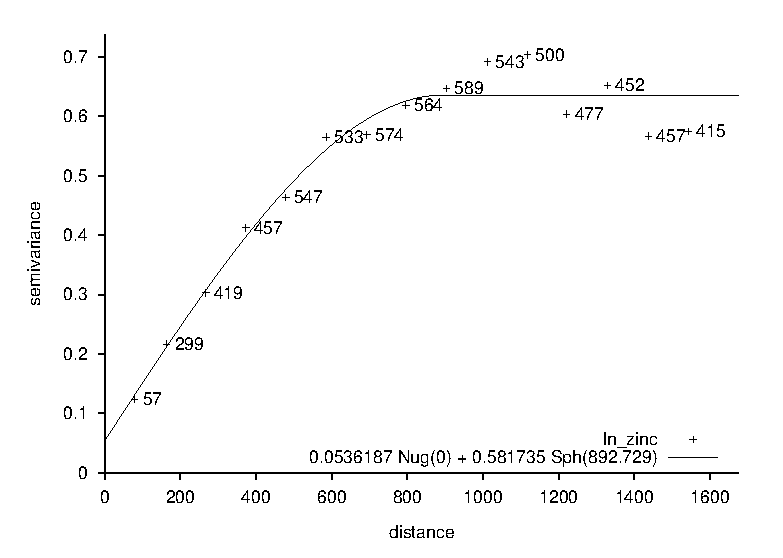
\includegraphics[scale=0.65]{\ext/vgm1} \\
\vspace{.4cm}
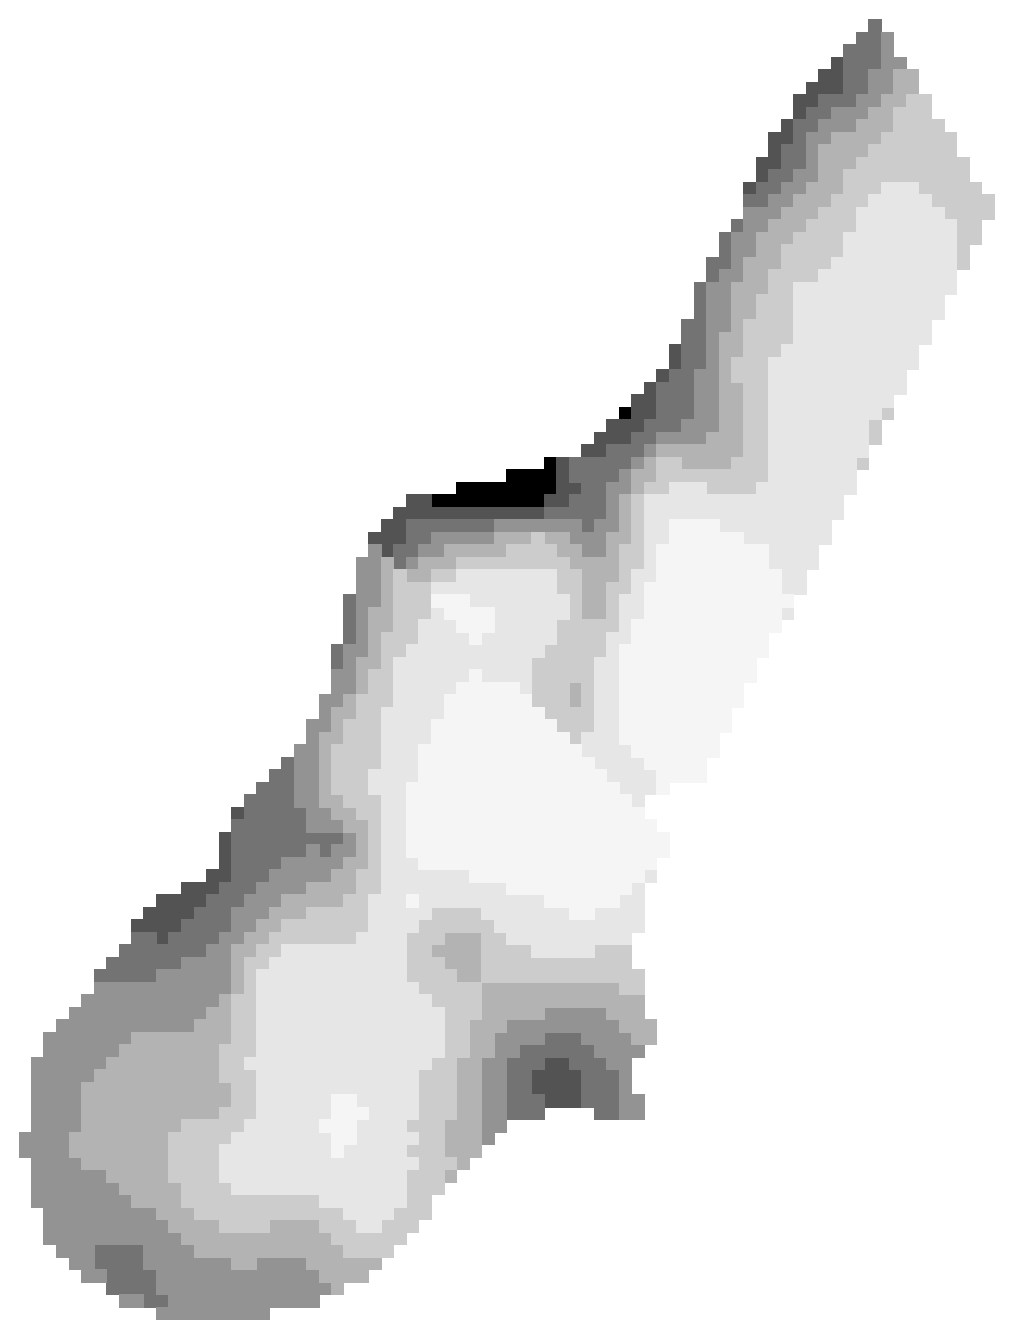
\includegraphics[scale=0.4]{\ext/lzn} \\
\vspace{.8cm}
{\em Edzer J. Pebesma} \\
Dept. of Physical Geography, Utrecht University \\
P.O. Box 80.115, 3508 TC, Utrecht, The Netherlands 
\end{center}

\newpage

\vspace*{\fill} % or try a length, 5c or \vspace*{\fill}

\noindent
gstat \version\ (\today) \\[2mm]
Copyright \copyright\ 1992, 2003 Edzer J. Pebesma \\ 
Permission is granted to copy, distribute and/or modify this document
under the terms of the GNU Free Documentation License, Version 1.2 or
any later version published by the Free Software Foundation; with no
Invariant Sections, no Front-Cover Texts, and no Back-Cover Texts. \\
See {\tt http://www.gnu.org/copyleft/fdl.html} \\[2mm]

Gstat is free software; you can redistribute it and/or modify it under
the terms of the GNU General Public License as published by the Free
Software Foundation; either version 2 of the License, or (at your
option) any later version. Gstat is distributed in the hope that it will
be useful, but without any warranty; without even the implied warranty
of merchantability or fitness for a particular purpose.  See the GNU
General Public License for more details. You should have received a copy
of the GNU General Public License along with the program (see the file
COPYING); if not, write to the Free Software Foundation, Inc., 675 Mass
Ave, Cambridge, MA 02139, USA. \\[2mm]
Meschach matrix library: Copyright \copyright\ 1993 David E. Stewart and
Zbigniew Leyk \\[2mm]
Gnuplot: Copyright \copyright\ 1986-1993, 1998 Thomas Williams and Colin 
Kelley and many others \\[2mm]
Relevant Internet locations:\\
Gstat: \http \\
Meschach: \code{ftp://ftpmaths.anu.edu.au/pub/meschach/meschach.html} \\
Gnuplot: \code{http://www.gnuplot.info/} \\
R: \code{http://www.r-project.org} \\
S-PLUS: \code{http://www.insightful.com}
\end{titlepage}


\tableofcontents

\chapter{Introduction}

Gstat is a program for the modelling, prediction and simulation of
geostatistical data in one, two or three dimensions. Geostatistical data
are data (measurements) collected at known locations in space, from a
function (process) that has a value at every location in a certain (1, 2
or 3-D) domain. These data (or some transform of them) are modelled as
the sum of a constant or varying trend and a spatially correlated
residual. Given a model for the trend, and under some stationarity
assumptions, geostatistical modelling involves the estimation of the
spatial correlation. Geostatistical prediction (`kriging') is finding
the best linear unbiased prediction (the expected value) with its
prediction error for a variable at a location, given observations and a
model for their spatial variation. Simulation of a spatial variable is
the creation of randomly drawn realizations of a field given a model for
the data, possibly conditioned on observations.

In gstat, geostatistical modelling comprises calculation of sample
variograms and cross variograms (or covariograms) and fitting models to
them. Sample (co-) variograms are calculated from ordinary, weighted or
generalised least squares residuals. Nested models are fitted to sample
(co-) variograms using weighted least squares, and during a fit each
single parameter can be fixed. Restricted maximum likelyhood estimation
of partial sills is also implemented. In the interactive variogram
modelling user interface of gstat, variograms are plotted using the
plotting program gnuplot.

Gstat provides prediction and estimation using a model that is the sum of
a trend modelled as a linear function of polynomials of the coordinates
or of user-defined base functions, and an independent or dependent,
geostatistically modelled residual. This allows simple, ordinary and
universal kriging, simple, ordinary and universal cokriging, standardised
cokriging, kriging with external drift, block kriging and ``kriging
the trend'', as well as uncorrelated, ordinary or weighted least squares
regression prediction. Simulation in gstat comprises uni- or multivariable
conditional or unconditional multi-Gaussian sequential simulation of point
values or block averages, or (multi-) indicator sequential simulation.

Besides many of the common options found in other geostatistical
software packages, the gstat program offers the unique combination of
\begin{itemize}
\item an interactive user interface for modelling variograms and
generalised covariances (residual variograms), that uses the
device-independent plotting program gnuplot for graphical display 
\item support for several ascii and binary data and grid map file
formats for input and output 
\item a concise, intuitive and flexible command language 
\item user customization of program defaults 
\item no built-in limits 
\item free, portable ansi-c source code 
\end{itemize}
The theory of geostatistics is not explained in this manual. Good texts
on the subject are e.g.\ \cite{journel78} and \cite{cressie93}. The
practice of geostatistical computation is explained only very briefly.
Texts about practical and computational aspects are e.g. \cite{isaaks}
and \cite{deutsch92}. This manual explains how things are done with gstat.

Chapter \ref{ch:getting} explains the concepts behind gstat and its basic
methods and prediction or simulation modes. Chapter \ref{ch:modes} treats
the simple, multiple, multivariable and stratified modes, and change of
support (block kriging). Chapter \ref{ch:syntax} is a complete reference
of the command file syntax. Chapter \ref{ch:environment} explains how
the program can be further controlled, for instance by using start-up
files, command line options or environment variables. Finally, Chapter
\ref{ch:examples} lists a number of example command files that demonstrate
most of the capabilities of gstat (these files are part of the program
distribution).

\urlmanual

The appendices contain more technical details: equations for modelling and
prediction (\ref{app:eqs.main}) and error messages and help information
(\ref{app:trouble}). 

\section{gstat mailing lists}

\gstatinfo is a mailing list for questions regarding the use of gstat,
and for comments, request and discussion regarding gstat's functionality.

A mailing lists for announces (version releases etc.) regarding gstat,
exists; for subscription information visit the gstat home page, \http.

\section{gstat for R and S-PLUS}

The majority of gstat's functionality is also directly accessible from
R or S-PLUS sessions, once the gstat package (R) or library (S-PLUS)
is loaded. In this form, gstat provides a number of features that are
not available from the gstat stand alone program. Chapter \ref{ch:s}
gives an overview of the functionality provided by the gstat S package.

% Ref to C & G paper.
\section{Further reading}
In {\em Computers and Geosciences} a paper written on gstat appeared
\cite{pebesma98}. Beyond much of the information present in this manual,
it discusses
\begin{itemize}
\item implementation and efficiency issues in gstat (computational and
algorithmic aspects in geostatistics)
\item managing large geostatistical projects
\item technical issues (portability, numerical precision, implementation
of the command file parser and interactive user interface, program limits)
\item a comparison with GSLIB \cite{deutsch92} and GeoEAS.
\end{itemize}
On the third international workshop on 'Distributed Statistical Computing'
(DSC 2003) a (draft) paper called ``Gstat: multivariable geostatistics for
S'' was presented. It introduces the gstat S package (for R and S-PLUS).
It can be found from:

{\tt http://www.ci.tuwien.ac.at/Conferences/DSC-2003/}

\chapter{Getting started}
\label{ch:getting}

This chapter deals with the gstat stand-alone program. Another way of
working with gstat is using the gstat S package from an S (R or S-PLUS)
session. This is briefly dealt with in chapter \ref{ch:s}.

\section{Invoking gstat}
\label{sec:gstat}
\index{invoking gstat}

Gstat is started either by typing 
\index{command files}

{\tt gstat} {\em command\_file}

\noindent
where {\em command\_file} is the name of a file with gstat commands,
or by typing

{\tt gstat -i}

\noindent
In the latter case, the interactive variogram modelling user interface
is started. This interface can be used to specify data, calculate
and plot sample variograms, fit variogram models and create variogram
plot files. Within the interface, help is obtained by pressing `H' or
`?', and the program stops after pressing `q' or `x'. At the end of a
variogram modelling session the program settings concerning data and
(fitted) variogram models can be written to a gstat command file by
pressing `c'. Such a command file will look like:

\begin{verbatim}
#
# gstat command file
#
data(zinc): 'zinc.eas', x=1, y=2, v=3;
variogram(zinc): 0.0716914 Nug(0) + 0.563708 Sph(917.803);
\end{verbatim}

The first three lines that start with a \verb|#| are comment lines,
the following lines are gstat commands. The first command specifies
where data were read (the variable {\tt zinc} was read from the file
{\tt zinc.eas}, having measured values on column 3, x-coordinates on
column 1 and y-coordinates on column 2), the second command defines a
variogram model for the variable {\tt zinc} (the sum of a nugget and a
spherical model). Suppose that these commands are held in a file called
{\tt zinc.gst}, then starting gstat with the command

{\tt gstat zinc.gst}

\noindent
will start the variogram modelling user interface after reading data
and variogram model, and work can be continued at the point where it
was saved before.

At a later stage, the data and variogram definitions in the command
file can be used for kriging. This is accomplished by adding commands
to the command file that specify where the kriging predictions should
be made, and where the results should be written to. Consider the command
file \verb|zinc_pr.gst|:

\begin{verbatim}
#
# gstat command file
#
data(zinc): 'zinc.eas', x=1, y=2, v=3;
variogram(zinc): 0.0717 Nug(0) + 0.564 Sph(917.8);
mask:       'mask.map';
predictions(zinc): 'zinc_pr.map';
variances(zinc):  'zinc_var.map';
\end{verbatim}

It says that prediction locations are the grid cell centres of the
(non-missing valued) cells in the grid map {\tt mask.map}, that ordinary
kriging predictions should be written to the grid map {\tt zinc\_pr.map},
and ordinary kriging prediction variances to {\tt zinc\_var.map}, after
starting gstat as:

\verb|gstat zinc_pr.gst|

\section{Data formats}
\label{sec:formats}
\index{data format}
\index{map format}
\index{grid map format}

Measurement data (measured values, their spatial coordinates, and
optionally base function values) are read from ascii table or (simplified)
GeoEAS table files, from grid map files (see Appendix \ref{app:formats})
or from Idrisi point (.vec) files. Table (or column) files are ascii
files without a header, with each line holding one record, and fields
on a line separated by blanks, commas or tabs. The simplified GeoEAS
format is a table file with a header. The GeoEAS file header has text
information on the first line; $m$, the number of variables in the file
on the second line, and $m$ variable names on lines 3 to $m+2$.

\index{pcraster}
\index{idrisi}
\index{arc-info}
\index{asciigrid}
\index{floatgrid}
Grid map files may have one of the following formats: Arc-Info grid
(gridfloat or gridascii), Idrisi image (ascii, real binary, byte),
PCRaster (all formats, \cite{vandeursen92}), ER-Mapper, GMT, Surfer
ascii. Output grid maps are written in the same format as the input (mask)
map. Files in formats that use two files and assume fixed extensions
(idrisi, gridfloat) should be denoted by the file base name only (omit
the extension for gstat). A grid map conversion is built in gstat,
see section \ref{sec:actions} Technical information on data and grid
map formats supported is found in appendix \ref{app:formats}. Gstat
has a built-in map format conversion utility (convert, Section
\ref{sec:actions}).

\section{Default program action}
\index{program action, default}
\index{default program action}

Based on the information read in the command file, gstat decides what to
do: variogram modelling, prediction or simulation, and, in case of
prediction, which prediction method to use. The decision tree for the
default program action is shown in Fig. \ref{fig:decis.1}.

\begin{figure}[ht]
\begin{center}
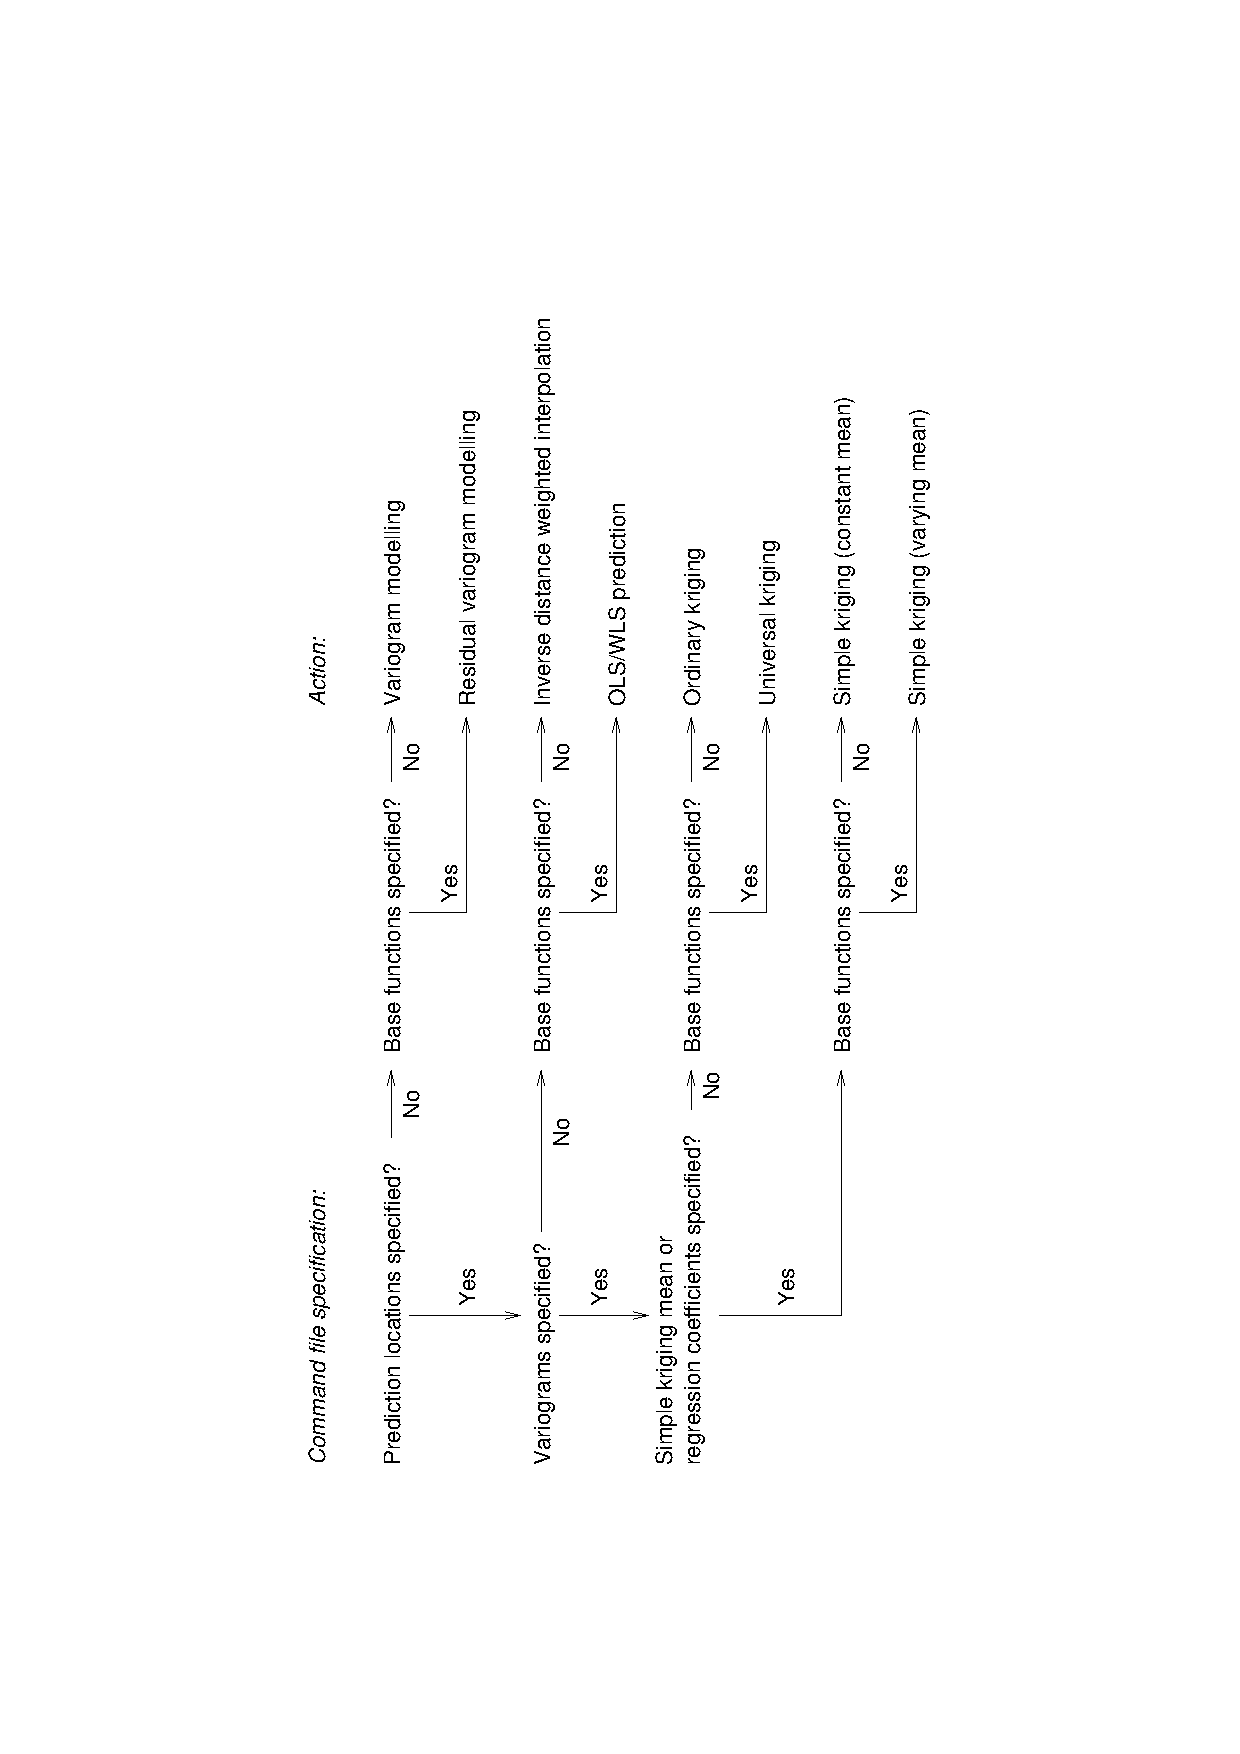
\includegraphics[width=\textwidth]{\ext/decis1}
\end{center}
\caption{Decision tree for default program action}
\label{fig:decis.1}
\end{figure}

When observations, variogram, and prediction locations are specified,
the default action is ordinary kriging on mask map locations. When,
in the final example in section \ref{sec:gstat}, the line

{\tt \iskey{variogram}(zinc):}...{\tt ;}

\noindent
is left out, inverse distance weighted interpolation is the default
action (kriging demands specification of the variogram). When the
command

{\iskey{mask}:} ... {\tt ;}

\noindent
is left out, the default action is variogram modelling because prediction
demands specification of prediction locations.

Sometimes it is necessary to override the default program action (e.g.
to calculate variograms non-interactively, or to do simulation instead
of prediction). Information about overriding the default program action
is found in sections \ref{sec:modelling}, \ref{sec:simulation} and
\ref{sec:method}.

\section{Modelling spatial dependence}
\label{sec:modelling}
\index{variogram modelling}
\index{interactive variogram modelling}
\index{variogram!modelling}

When no prediction locations are defined in the command file, gstat
starts the interactive variogram modelling user interface (\ex{1},
\ex{2}). Multiple variables are analyzed when they are specified with
{\tt \iskey{data}({\em id}\/)} commands, each having a unique {\tt
{\em id}}. From this interface sample variograms, covariograms, cross
variograms and cross covariograms can be calculated, viewed, and modelled
(see Appendix \ref{app:sample}); variogram plots can be saved (e.g. as
{\sc PostScript} file, Fig.\ \ref{fig:vario.plot})
and printed; and modified settings of data and fitted variograms can
be saved as a gstat command file. The interface has several selection
items and single-key options. Summary help is obtained by pressing `H'
(shift-h). 

\begin{figure}[ht]
\begin{center}
 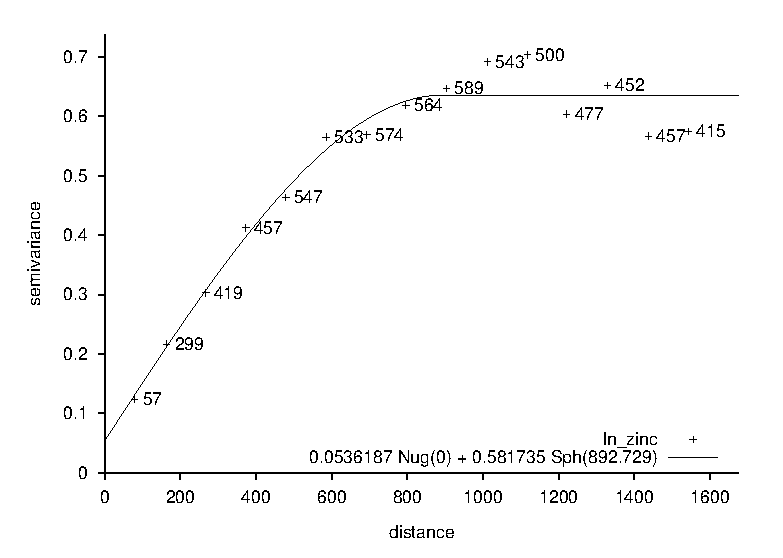
\includegraphics[width=0.75\textwidth]{\ext/vgm1}
\end{center}
\caption{Variogram plot from gnuplot}
\label{fig:vario.plot}
\end{figure}

Help on a specific user interface item is obtained by selecting the item
with the cursor keys and pressing `?'. What follows is a brief
description of the visible items in the user interface:

\begin{codelist}
\item[\texttt{enter/modify data}]
enter a new variable or modify (reload) a variable (allows only a few
input options)
\item[\texttt{choose variable}]
choose a variable, or, if the next field is on a cross (co-) variogram,
a pair of variables
\item[\texttt{calculate what}]
choose what to calculate (variogram, cross variogram, covariogram or
cross covariogram)
\item[\texttt{cutoff, width}]
prompts for the cutoff (the maximum distance at which pairs of data
points will be considered for inclusion in sample variogram estimates) and
the lag width (the step size of distance intervals for sample variogram
estimates). Non-even interval boundaries can be obtained by specifying
\iskey{bounds} in the command file (section \ref{sec:basic})
\item[\texttt{direction}]
enter directional parameters (direction angle and direction tolerance:
the maximum deviation from this direction tolerated for a pair of data
points to be included in the sample variogram estimate)
\item[\texttt{variogram model}]
enter a variogram model or change variogram model parameters (section
\ref{sec:variograms})
\item[\texttt{fit method}]
choose a variogram fit method (or no fit)
\item[\texttt{show plot}]
show variogram and model (if present, and after optional fitting)
\end{codelist}

Variogram models can be fitted to the sample variogram using iterative
reweighted least squares estimation \cite{cressie85}, or can be fitted
directly to the sample data using REML estimation \cite{kitanidis85}.
Appendix \ref{app:sample} gives details on the calculation of sample
(co-) variograms and model fitting. Non-linear least squares fitting is
only guaranteed to work when good initial values are provided. Therefore,
and more in general, visual examination of model fit is recommended.

\index{save variogram plot}
\index{variogram!save plot as}
\index{gnuplot}

Variogram plots can be saved as encapsulated {\sc PostScript} file
(Fig. \ref{fig:vario.plot}) from gnuplot by pressing `P' or as
\htmladdnormallink{gif}{png/fit.png} file by pressing `G' (gif only
when the \htmladdnormallink{gd}{http://www.boutell.com/gd/} library was
linked to gnuplot). Plots can be customised (e.g. labels, legend, title)
by first saving sample variogram estimates to a file (`e'), then saving
the gnuplot commands to a file (`g'), then modifying this file and finally
using gnuplot to create the {\sc PostScript} (or other graphics) file.

By default, direct and cross variograms and covariograms are calculated
from ordinary least squares residuals by using a linear model (as default
only an intercept, section \ref{sec:linear}). Generalised least squares
residuals are used when the command

{\tt set \iskey{gls}=1;}

\noindent
is added to the command file (sections \ref{sec:linear}, \ref{sec:set}).

\subsection*{Non-interactive variogram modelling}

Variograms can also be calculated non-interactively, by adding the command

{{\tt \iskey{method}: \iskey{semivariogram};}}
\index{variogram!sample!non-interactive}

\noindent
or

{{\tt \iskey{method}: \iskey{covariogram};}}
\index{covariogram!sample!non-interactive}

\noindent
to the command file (section \ref{sec:method}). 

Sample variograms can be saved to a file, using for instance:

{{\tt\iskey{variogram}(zinc): 'zinc.est';}}

\noindent
For large data sets, it may be best to calculate sample variograms
non-interactively and do the modelling afterwards. This is accomplished
by first saving the sample variograms to file as described above, and
then to load only the sample variograms in the user interface (not the
data), which is done by defining dummy data:

{{\tt\iskey{data}(zinc);} \# dummy data}

\noindent
and a valid sample variogram, as

{\tt\iskey{variogram}(zinc): 'zinc.est';}

\noindent
or, when a variogram model should be defined ahead of fitting:

{{\tt\iskey{variogram}(zinc): 'zinc.est', 1 Nug() + 1 Sph(800);}}

\subsection*{Variogram maps}
\index{variogram!maps}
If in addition to one of these \iskey{method} commands a mask map is
specified, then gstat calculates the variogram map \cite{isaaks} for
the field specified by the mask, and writes this map to the output map
{\tt zincv.map}

{{\tt\iskey{variogram}(zinc): 'zinc.map';}}

\noindent
optionally, in addition the corresponding number of data pairs can be
written to the output map {\tt zincn.map} when specified as

{{\tt\iskey{variogram}(zinc): 'zince.map', 'zincn.map';}}

\noindent
(typically a variogram map is centred around (0,0) and has map dimension
and cell size similar to cutoff and interval width values).

\section{Prediction}
\label{sec:prediction}
\index{prediction}

If prediction locations are defined in the command file, gstat chooses
a prediction method depending on the model defined by the complete set
of commands in a command file.

\index{inverse distance weighted interpolation}
When no variograms are specified, inverse distance weighted interpolation
is the default action (Fig.\ \ref{fig:decis.1}, \ex{3}).

\index{kriging}
\index{kriging, ordinary}
When variograms are specified the default prediction method is ordinary
kriging \cite{journel78,cressie93} (\ex{4} and \ex{8}).

\index{kriging, simple}
Simple kriging is the default action when in addition for each
variable the simple kriging mean (\isXkey{sk\_mean}{skXmean} or
\iskey{b}) is set (section \ref{sec:data}; \ex{5}, universal kriging
or uncorrelated linear model prediction is used when a model for the
trend is defined ,section \ref{sec:linear}). Multiple prediction,
multivariable prediction, and stratified prediction are described in
section \ref{sec:modes.simple}-\ref{sec:stratified}. Prediction of block
averages is described in section \ref{sec:support}.

\index{kriging, simple}

\noindent
If the prediction locations are specified as a mask map with the command

{\tt \iskey{mask}: 'file';}

\noindent
then predictions and prediction variances are written to output maps
only when these maps are specified explicitly (section \ref{sec:basic};
\ex{5}).

% prediction.data. @SubIndex { data locations, on }

As an alternative to prediction on grid map locations, prediction on
non-gridded locations is the default action when these locations are
specified with the

{\tt \iskey{data}():} ... {\tt ;}

\noindent
command (note the absence of an identifier between the parentheses). In
this case, output is written in ascii table or simplified GeoEAS format to
the file defined by the command {\tt set \iskey{output}='{\em file}';}
(\ex{4}, or defined with the command line option {\tt -o}, section
\ref{sec:clo}).

\begin{figure}[ht]
 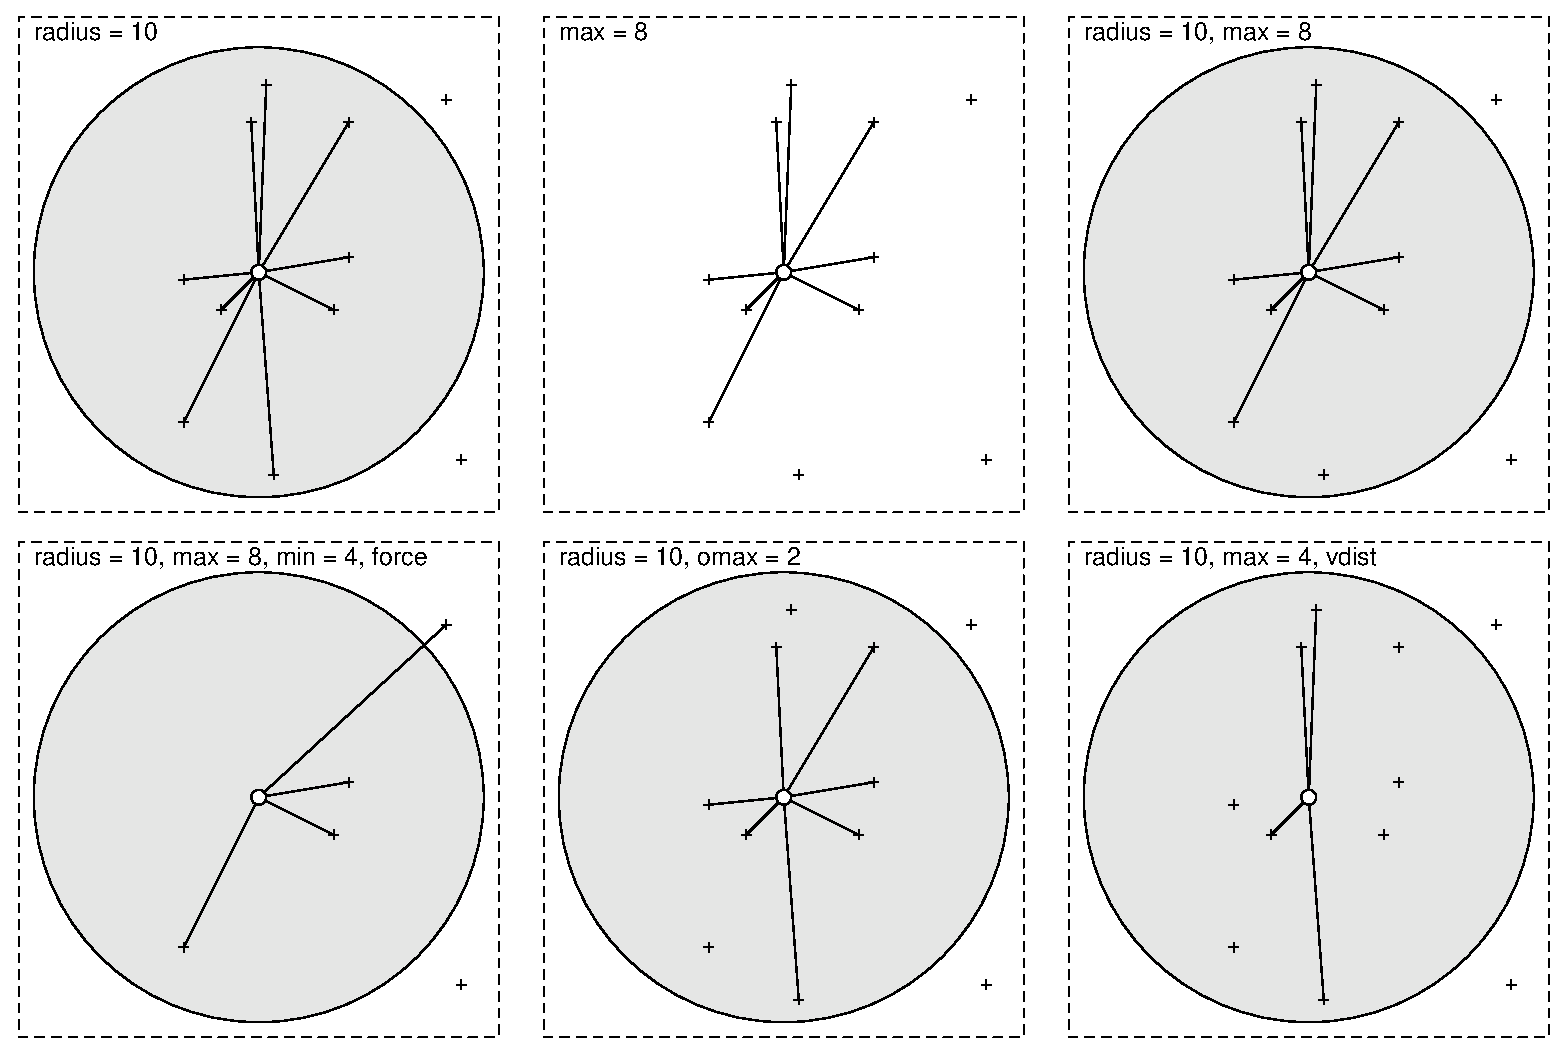
\includegraphics[width=\textwidth]{\ext/nbh}
\caption{Local neighbourhood selections. Lines indicate selected points
(+). Lower right: variable with anisotropic variogram having a strong
north-south correlation }
\label{fig:nbh}
\end{figure}

\subsection*{Local Neighbourhoods}

\index{kriging!local}
\index{prediction!local}
\index{neighbourhood!selection}
\index{local neighbourhood}

By default, gstat uses global prediction, meaning that for each prediction
all data values are used. However, it is often desirable to use not
all data values, but only a subset in a (spatial) neighbourhood around
the prediction (simulation) location, for either computational reasons
or the wish to assume first-order stationarity only locally. Gstat
allows local neighbourhood selections to be based on distance
(\iskey{radius}), number of data points (\iskey{max}, \iskey{min}),
variogram distance (\iskey{vdist}), and number of data points per octant
(3D) or quadrant (2D) (\iskey{omax}). The options are explained below
(see also Fig.\ \ref{fig:nbh}, section \ref{sec:data} examples in chapter
\ref{ch:examples}).

The quadtree-based algorithm used to obtain data
points in a local search neighbourhood is described in
\cite{hjaltason95}, and is found at \htmladdnormallink
{\code{http://www.cs.umd.edu/~brabec/quadtree/index.html}}
{http://www.cs.umd.edu/~brabec/quadtree/index.html}
(Bucket PR Quadtree demo).

\begin{codelist}
\item[\code{\iskey{radius} = 10}]
select all data points within 10 (euclidian) distance units from the
prediction location
\item[\code{\iskey{max} = 8}]
select the 8 data points that are closest (in euclidian distance) to the
prediction location (or take all data points if less than 8 are available)
\end{codelist}

\noindent
Some options should be combined, and permitted combinations are
explained below. (Combinations not mentioned might result in unexpected
or undesired results.)

\begin{codelist}
\item[\code{\iskey{radius} = 10, \iskey{max} = 8}]
after selecting all data points at
(euclidian) distances from the prediction location less or equal to 10,
choose the 8 closest when more than 8 are found
\item[\code{\iskey{radius} = 10, \iskey{max} = 8, \iskey{min} = 4}]
in addition to the previous selection, generate a missing value if less
than 4 points are found within the search radius 10
\item[\code{\iskey{radius} = 10, \iskey{max} = 8, \iskey{min} = 4,
\iskey{force}}]
in addition to the previous selection, if less than 4 data
points are found in the search radius, instead of generating a missing
value, select (force) the 4 nearest (in euclidian distance) data points,
regardless their distance
\item[\code{\iskey{radius} = 10, \iskey{omax} = 2}]
after selecting all data points at distances 
less or equal to 10, choose the 2 closest data points in each
octant (3D), quadrant (2D) or secant (1D)
\item[\code{\iskey{radius} = 10, \iskey{vdist}, ...}]
after the radius selection, decide what the {\em nearest} data points
are on the base of point-to-point semivariance of the data variable
instead of euclidian distances (``semivariance distance'': in case of
anisotropy this allows the prevalence of more correlated points over
the, in the euclidian sense, nearest points)
\end{codelist}

\noindent
{\em Indicator kriging}
% kriging.indicator. @SubIndex { indicator }

\noindent
Basically, indicator kriging is equivalent to simple or ordinary
kriging of indicator-transformed data. However, resulting estimates of
indicator values are not guaranteed to satisfy order relations. During
indicator kriging, gstat will do order relation violation correction for
independent, cumulative or categorical (disjunct) indicators only if the
\iskey{order} is to one of the values in Table \ref{tab:orvc}
in section \ref{sec:simulation}, \iskey{order} in section
\ref{sec:set} and \cite{deutsch92,goovaerts97}.

\section{Simulation}
\label{sec:simulation}
\index{simulation}

% simulation. @Index { simulation }

Simulation \cite{davis87,gomez93,myers89} is done by setting up a command
file for simple kriging (section \ref{sec:prediction}) and changing the
default action to Gaussian simulation by adding the command

{\tt \iskey{method}: \iskey{gs};}

\noindent
(\ex{6} and \ex{7}), or to indicator simulation by adding the command

{\tt \iskey{method}: \iskey{is};}

\noindent
If valid data are present (i.e., data are available in the neighbourhoods
defined), conditional simulation is done. Unconditional simulation is
done when only dummy variables (\iskey{dummy}, section \ref{sec:data})
or data outside every possible neighbourhood are defined.

% simulation.conditional. @SubIndex { conditional }
% conditional.simulation. @Index { conditional simulation }

% simulation.unconditional. @SubIndex { unconditional }
% unconditional.simulation. @Index { unconditional simulation }

\index{simulation!sequential}

The sequential simulation algorithm \cite{gomez93} is used for the
simulation. This algorithm visits each simulation location, following a
random path. After simulating a value (or set of values in the
multivariable case) at the location, it is added to the conditioning
data.

A few notes on the practice of (indicator or Gaussian) simulation with
gstat are:

\begin{itemize}

\index{simulation!local neighbourhood}
\item Even for simulating small fields (e.g. 500 cells) it is strongly
recommended to limit the kriging neighbourhood in order to get local
kriging (section \ref{sec:prediction}). Because every simulated point
or block is added to the data, `global' simulation would soon amount to
large kriging systems, thus slowing down the simulation quickly.

\index{simulation!number of realizations}
\item Gstat can create many simulations simultaneously in an efficient
way: a single random path is followed and for each simulation location,
the neighbourhood selection and the solution to the kriging system are
reused for all subsequent simulations. When many simulations are required
(e.g. for a Monte Carlo study) the time saving will be significant
(see {\tt set \iskey{nsim}}). (Note that the use of local approximations
(local kriging) results in slightly dependent realizations when obtained
by following a single random path.)

\index{simulation!random path}
\item When simulation is done on a regular grid (using a mask map), in
order to reproduce the statistical properties up to reasonably large
distances, a recursively refining random path (``multiple-steps
simulation'', \cite{gomez93}) is followed, shown in
Fig. \ref{fig:msteps}.

\begin{figure}[t]
\begin{center}
 \includegraphics[width=\textwidth]{\ext/msteps}
\end{center}
\caption{Recursively refining visiting sequence during simulation}
\label{fig:msteps}
\end{figure}

A random path is started on a (randomly located) coarse grid (A: the
coarsest (2 $\times$ 2) grid with a grid spacing that is a power of 2).
The simulation grid is refined recursively: 4 $\times$ 4 (B), 8 $\times$
8 (C, black dots) halving the grid spacing each step) until all grid
locations are visited (C, grey dots). Neighbourhood definitions (see
section \ref{sec:data}, and also the \iskey{force} flag) may ensure that
necessary conditioning data are used for reproducing the statistical
properties sufficiently.

\index{simulation!variogram reproduction}
\index{simulation!varying mean}
\item Simple kriging results in a correct conditional distribution, and
in Gaussian simulations that honour the specified variogram. Universal or
ordinary kriging can be used if enough conditioning data are
available, and leads to `rougher' simulations, less honouring the
variogram but better adjusted to a non-stationary mean (``major
heterogeneities'', \cite{deutsch92}), when present in the conditioning
data. The parameter \iskey{nXuk} (section \ref {sec:set}) controls the
choice between simple or universal (ordinary) kriging. Another way to
obtain non-stationary simulations is to add a varying mean to a
stationary (simple kriging) simulation afterwards.
\end{itemize}

\subsection*{Gaussian block simulation}
\index{simulation!block averages}

Gstat simulates block averages when a non-zero block size is specified
(section \ref{sec:support}). The implementation of this is a rather
inefficient one. Simulation will be faster when \iskey{nblockdiscr} is
set to a low value (to 3 or 2, section \ref{sec:set}), at the expense of
the accuracy of point-to-block and block-to-block covariance calculations
(see Appendix \ref{app:blocks}).

\subsection*{Indicator simulation}
\index{simulation!indicator}
\index{indicator simulation}

\begin{table} 
\begin{center}
\begin{tabular}{|l|l|l|c|} \hline
 Indicator & order violation & correction & {\tt set order} \\ \hline
 independent & $\hat{p}_i < 0$ & $\tilde{p}_i = 0$ & {\tt 1-4} \\
 independent & $\hat{p}_i > 1$ & $\tilde{p}_i = 1$ & {\tt 1-4} \\
 categorical, open & $\sum_{i=1}^{n} \hat{p}_i > 1$ &
 $\tilde{p}_i = \hat{p}_i / \sum_{i=1}^{n} \hat{p}_i$ & {\tt 2} \\
 categorical, closed & $\sum_{i=1}^{n} \hat{p}_i \ne 1$ &
 $\tilde{p}_i = \hat{p}_i / \sum_{i=1}^{n} \hat{p}_i$ & {\tt 3} \\
 cumulative & $\hat{p}_i < \hat{p}_{i-1}$ & 
 $\tilde{p}_i - \tilde{p}_{i-1} = 0$ & {\tt 4} \\ \hline
\end{tabular}
\end{center}
% \caption{Order relation corrections (estimated probality $\hat{p}_i$, corrected estimate $\tilde{p}_i$)}
\caption{Order relation corrections}
\label{tab:orvc}
\end{table} 

\index{indicator simulation!categorical}
\index{indicator simulation!cumulative}
\index{indicator simulation!independent}
\noindent
From data definitions alone, gstat cannot decide whether it is working
with indicator variables or not. In case of prediction this is not
crucial---procedure-wise, indicator kriging is identical to simple
or ordinary kriging. When indicator simulation is done for multiple
variables, a number of different situations may occur, and for correct
results, it should be specified explicitly if the set of indicator
variables is (i) independent, (ii) cumulative or (iii) disjunct:

\begin{itemize}
\item if the set is {\em independent}, simulated indicator variable can
take a value 1 or 0 independently from the other indicator variables
\item if the ordered set of indicator variables $I_0 (s),...,I_{n-1}
(s)$ is {\em cumulative}, then $I_j (s) = 1$ {\em implies} that $I_0
(s),...I_{j-1} (s)$ are all 1 (in gstat, the order of a set of indicator
variables equals the order in which the variables appear in the
command file)
\item if a set of indicators is {\em disjunct}, then $I_j (s) = 1$
implies that $I_i(s) = 0$ for all $i \neq j$.
\end{itemize}

Independent indicators may represent independent variables. A set
of cumulative indicators may represent the cumulative distribution
function of a single continuous variable and a set of disjunct
indicators can represent the categories of a categorical variable (see
also the data command options and \iskey{Category}). Table
\ref{tab:orvc} shows the corrections done for the different types of
indicator variables and the value \iskey{order} should be set to to
obtain the corrections (estimated probality $\hat{p}_i$, corrected
estimate $\tilde{p}_i$). Cumulative indicators are corrected using
the ``upward-downward'' approach, see \cite[p. 80]{deutsch92} or
\cite[p. 324]{goovaerts97}.

For multiple indicator simulation (no indicator cross variograms are
specified), by default independent indicator simulation is done. The
subsequent indicator variables are taken as cumulative indicators if the
command

{\tt set \iskey{order}=4;}

\noindent
is added to the command file (Table \ref{tab:orvc}). They will be treated
as disjunct if \iskey{order} is set to 2 or 3 (see section \ref{sec:set}).
\index{indicator simulation!order relation violations}
 
\section{Linear models in gstat}
\label{sec:linear}
\index{linear models}
\index{trend}

\subsection*{Defining a model}

In ordinary and simple kriging each observation $z(s_i)$ (the value of
variable $z$ at location $s_i$) is represented by the model
\begin{equation}
Z(s_i) = m + e(s_i)
\label{eq:ok}
\end{equation}
\index{trend!constant}
with, in case of ordinary kriging $Z(s)$ intrinsically stationary and
$m$ an unknown (locally) constant trend, or, in case of simple kriging,
$Z(s)$ a second order stationary and $m$ a known, constant trend.

A wider class of models is obtained when the observation $z(s_i)$ is
modelled as the sum of a spatially non-constant (i.e. non-stationary)
trend $m(s_i)$ and an intrinsically stationary error $e(s_i)$:
\begin{equation}
Z(s_i)=m(s_i)+e(s_i)
\label{eq:uk}
\end{equation}
\index{trend!varying}
\index{external drift}
\index{universal kriging}
\index{kriging!universal}
\index{base functions}
In the universal kriging model such a trend is modelled as a linear
function in $p$ known base functions $f_j (s) = (f_j (s_1),...,f_j(s_n))'$
and $p$ unknown constants $\beta_i$, which yields, for the observation
at $s_i$
$$ Z(s_i)=\sum_{j=1}^{p} f_j (s_i) \beta_j + e(s_i) $$
and for all observations
$$ Z(s)=\sum_{j=1}^{p} f_j(s)\beta_j + e(s)$$
which can be written in matrix notation as
\begin{equation}
Z(s)= F \beta + e(s)
\label{eq:lm}
\end{equation}
with $F = (f_1 (s),...,f_p (s))$ and $\beta = (\beta_1 ,...,
\beta_p)'$. Ordinary kriging (\ref{eq:ok}) is the special case where
this model has only an intercept ($p=1$, $f_1 (s) = 1, \forall x$ and
$\beta_1 = m$).

Gstat calculates prediction under the multivariable universal kriging
model \cite{verhoef93} when base functions $f_i(s)$ and variogram(s) for
$e(s)$ are specified (see appendix \ref{app:eqs} for the prediction
equations). An intercept (the constant value as in the ordinary
kriging model) in (\ref{eq:ok}) is assumed for each variable by default,
and only non-intercept base functions need to be specified. Base
functions can be polynomials of the coordinates (e.g. $x$, $x^2$, $xy$
etc.) or user-defined.

\subsection*{Coordinate polynomial base functions}
\index{base functions}
\index{base functions!coordinate polynomials}
\index{trend!coordinate polynomials}

For a data variable in two dimensions, a first order linear trend in the
coordinates is defined by

{\tt \iskey{data}(x): 'file', \iskey{x}=1, \iskey{y}=2, \iskey{v}=3, \iskey{X}=x\&y;}

\noindent
or, as a shorthand for this, the coordinate polynomial trend order
degree can be specified:

{\tt \iskey{data}(x): 'file', \iskey{x}=1, \iskey{y}=2, \iskey{v}=3,
\iskey{d}=1;}

\noindent
(Note that {\tt \iskey{d}=1} is equivalent to {\tt \iskey{X}=x} for
one-dimensional, {\tt \iskey{X}=x\&y} to for two-dimensional and to {\tt
\iskey{X}=x\&y\&z} for three-dimensional data.) Values of coordinate
polynomial base functions at observation and prediction locations are
obtained from the (standardised) location coordinates $s_i$ (see also
\ex{17}).

\subsection*{User-defined base functions}
\index{base functions!arbitrary}
\index{trend!arbitrary base functions}

Non-coordinate polynomial, user-defined functions can also be specified
as base functions. Because they are not known, they should be defined as
column numbers in a data file (\ex{13}), like

{\tt \iskey{data}(x): 'file', \iskey{x}=1, \iskey{y}=2, \iskey{v}=3,
\iskey{X}=4\&5;}

\noindent
User-defined and coordinate polynomial base functions may be intermixed.

When binary (e.g., 0/1) variables are used as base functions, and the sum
of these functions coincides with an intercept (i.e., summed row-wise,
the columns equal a column with a constant), the default intercept has
to be overridden. This is done by specifying {\tt -1} as the first column
number of the base functions (\ex{14}).

Specification of the user-defined base function values at prediction
locations is necessary, since they are needed in the prediction. For the
prediction locations they are needed too, and for map prediction
locations they are defined as a list of mask maps containing the base
functions. For the {\tt \iskey{data}()} prediction locations they are
defined as the \iskey{X} column numbers in the corresponding file. In
both cases the number of base functions thus specified and the order in
which they appear should match the order in which the (non-intercept
and non-coordinate polynomial) \iskey{X} columns appear in subsequent
{\tt\iskey{data}({\em id}\/)} commands.

If more than one variable is defined and only direct variograms are
specified, multiple universal kriging is done. If in addition to direct
variograms cross variograms are specified, multivariable universal
kriging is done \cite{verhoef93} (universal cokriging, section
\ref{sec:multivariable}).

\subsection*{Ordinary and weighted least squares trend prediction}
\index{linear model!independent residuals}
\index{trend!ordinary least squares}
\index{trend!weighted least squares}
\index{ordinary least squares}
\index{weighted least squares}

If base functions are specified but no variograms are specified, the
default prediction method is the (multiple) regression prediction,
(ordinary least squares, OLS) assuming that the $e(s)$ are independently
identically distributed (IID). In this case the prediction variance is
the classical regression prediction variance for a single observation
(\ex{15} and \ex{17}), or for the mean value when the block size is
non-zero (section \ref{sec:support}).

If the errors are assumed to be independent with different variances,
$v_i \sigma^2$ then specifying the constants $v_i$ will result in weighted
least squares (WLS) prediction. The values $v_i$ are not variances
but merely relate an individual residuals variance to $\sigma^2$. For
instance, if an observation is an average of $n_i$ measurements, then,
assuming the variance of individual measurements is constant, $v_i$ can
be set to $n^{-1}_i$. In the unweighted case, all $v_i$ are 1, and for
prediction variances to make sense, the $v_i$ should be related to this
unity value ($\sigma^2$ should be ``the'' residual variance).

\subsection*{Generalised least squares trend prediction}
\index{trend!generalised least squares}
\index{generalised least squares}

If at prediction locations $s_0$, for some reason not the kriging
prediction but the generalised least squares estimate (or BLUE, best
linear unbiased estimate) of the trend $f(s_0 ) \hat \beta$ and its
estimation variance are needed, then this is obtained by overriding the
default method (ordinary or universal kriging) using

{\tt \iskey{method}: \iskey{trend};}

\noindent
Setting $f_i (s_0)$ to 1 and all other $f(s_0)$ to 0 yields the
generalised least squares estimate (BLUE) of $\hat{\beta}_i$. See appendix
\ref{app:eqs} for details on weighted or combined weighted and generalised
least squares prediction.

\subsection*{Residual variograms}
\index{variogram!OLS/WLS/GLS residual}

If base functions are specified but no prediction locations are
specified, then the sample direct or cross variogram and covariogram is
calculated from ordinary least squares (OLS) residuals, as obtained from
the linear model with IID errors. If generalised least squares residuals
are preferred to OLS residuals, the (initial) variograms should be set,
and \iskey{gls} should be set to 1 (section \ref{sec:set}).


\chapter{Prediction modes and change of support}
\label{ch:modes}
\index{prediction!modes}

\section{Modes}
\label{sec:modes.simple}

When a command file holds more than one variable, each specified with
a unique {\tt {\em id}}, then different prediction (or simulation)
{\em modes} are possible, depending on the complete model specification:
predictions can be made independently (`multiple' prediction), dependently
(`multivariable' prediction), or variables may correspond to certain
portions (categories) in the mask map or prediction location data
(`stratified' prediction). The modes hold equally for prediction
and simulation.  When only one variable is defined, predictions (or
simulations) are made for this variable at every prediction location
(`simple' mode). 

The decision tree gstat uses to determine the mode is shown in
Fig.\ \ref{fig:modes}.  The choice for a certain mode is always
implicit, and is made after gstat read the command file and examined
the data.

\begin{figure}[ht]
\begin{center}
 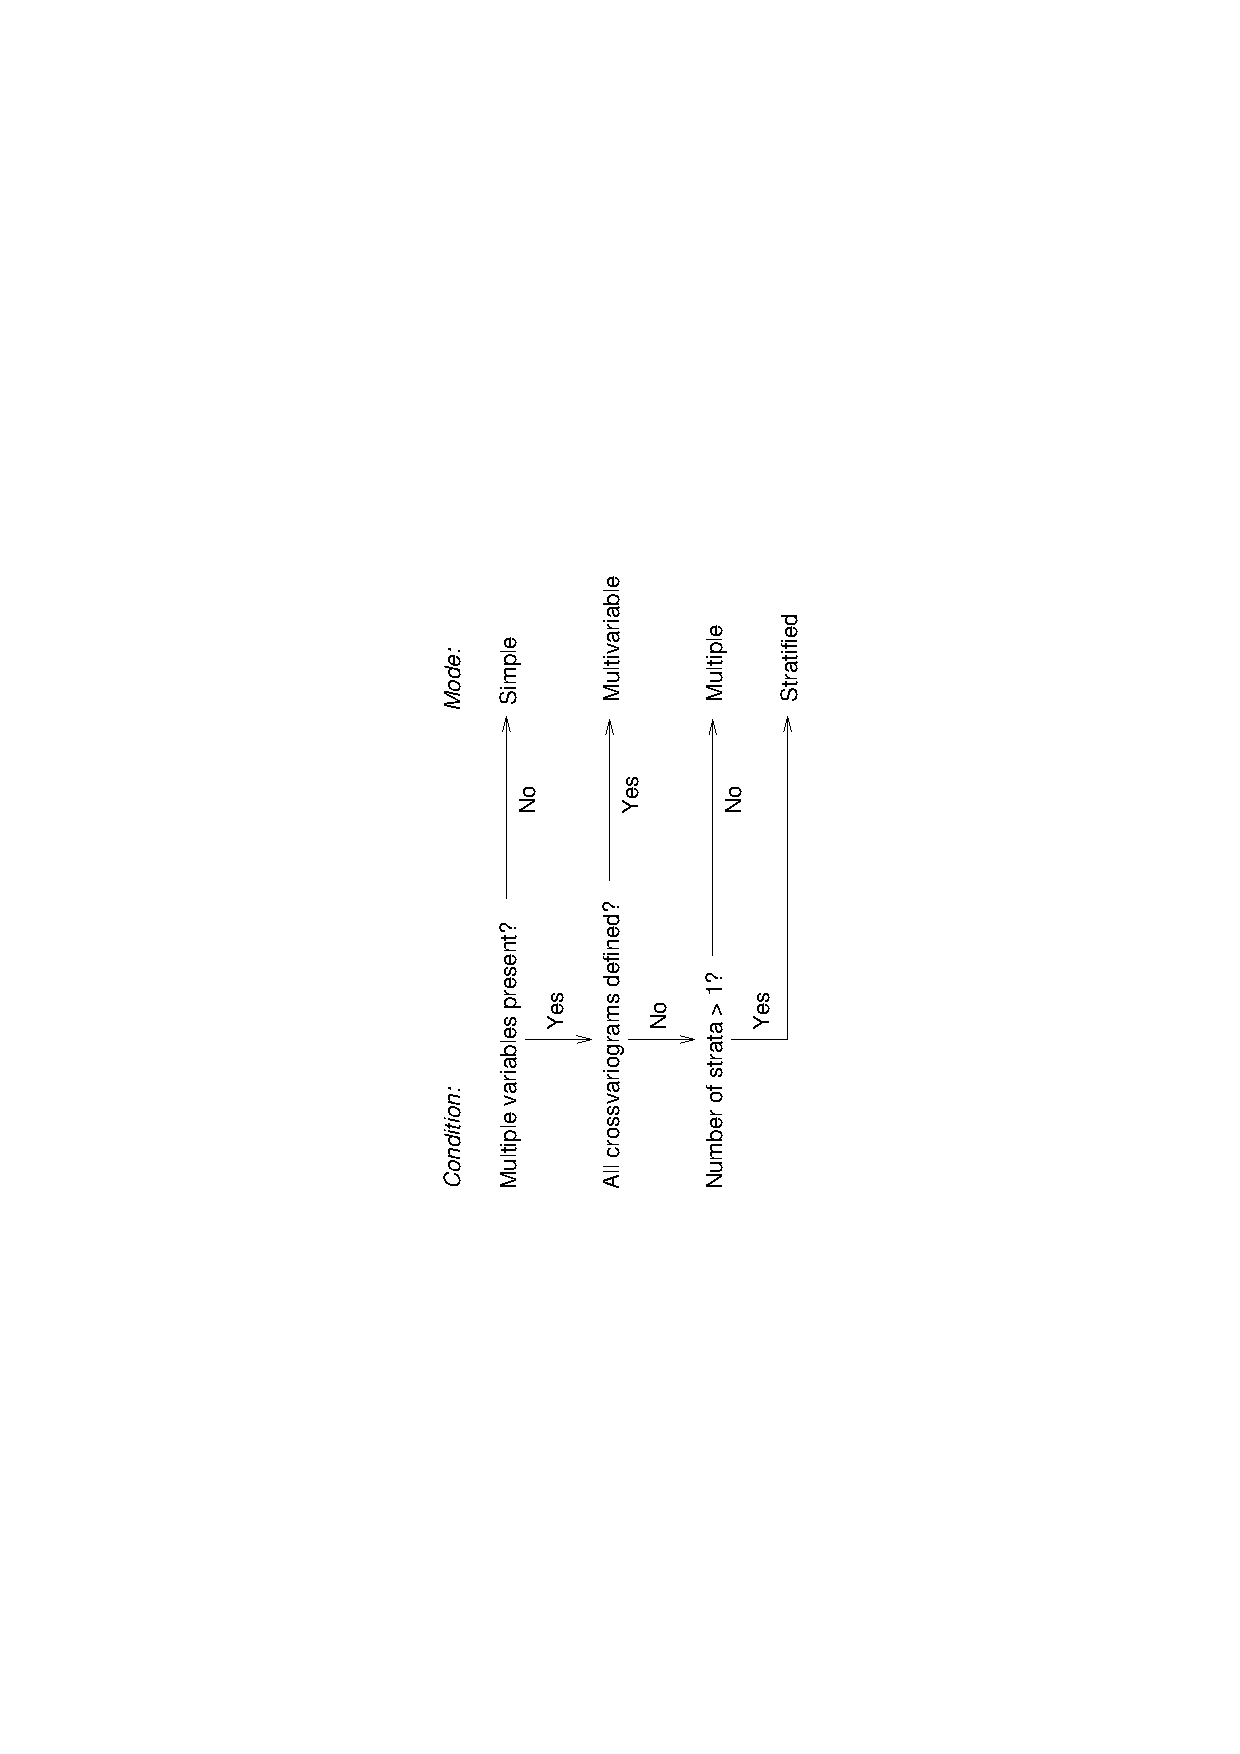
\includegraphics[width=0.7\textwidth]{\ext/decis2}
\end{center}
\caption{Prediction modes}
\label{fig:modes}
\end{figure}

\section{Multiple mode}
\label{sec:multiple}
\index{prediction!multiple}
\index{simulation!multiple}

When multiple variables are defined, and no variograms or only direct
variograms are defined (no cross variograms), then {\em multiple}
prediction (simulation) is the default action. See for instance
\ex{10}. In the multiple mode, predictions or simulations are made for
each variable independently. The advantage of using the multiple mode over
using a command files for each variable, is that, besides being concise,
if the variables have identical locations, each neighbourhood search is
done only for the first variable (\ex{16}).

% kriging.multiple. @SubIndex { multiple }


\section{Multivariable mode}
\label{sec:multivariable}
\index{prediction!multivariable}
\index{simulation!multivariable}

If in addition to direct variograms the cross variograms are defined for
all variable pairs, then the prediction mode becomes {\em multivariable}
(i.e., cokriging or co-simulations). In case of multivariable
prediction, prediction error covariances from multivariable prediction
\cite{verhoef93} on a map can be specified per identifier pair
with {\tt \iskey{covariances}({\em id1},{\em id2}\/)} (\ex{11}). In
gstat, multivariable prediction comprises simple cokriging, ordinary
cokriging or universal cokriging (as well as standardised cokriging,
multivariable indicator or Gaussian simulation).

% kriging.multivariable. @SubIndex { multivariable }
% kriging.cokriging. @SubIndex { cokriging }

When, for multiple variables a linear model is specified with independent
errors (no variograms are defined), and one or more of the variables'
regression parameters are defined as common parameters (with the
command \iskey{merge}, section \ref{sec:basic}) then the prediction
mode becomes multivariable as well (cf. analysis-of-covariance models
refXXchristensen96).

\section{Stratified mode}
\label{sec:stratified}
\index{prediction!stratified}
\index{simulation!stratified}

Stratified kriging or simulation (each variable with it's direct variogram
applies to a specific area in the mask map) is the default action if
the following conditions hold (\ex{12}):

% kriging.stratified. @SubIndex { stratified }

\begin{itemize}
\item more than one data variable is defined
\item only for the first data variable output maps (\iskey{predictions},
\iskey{variances}) are defined 
\item the (first) mask map defined has more than one category 
\end{itemize}

Data variables are numbered in the order they appear in the command
file, starting at 0. Let the minimum grid value of the (first) mask map
be $m$, If at a specific grid cell the mask map has value $j$, then for
that cell the stratified prediction map (and variance map) will have
predictions for variable $j - m$ (rounded to the nearest integer). Thus,
predictions at mask map cells having value $m$ will get predictions for
the first variable.

In case of universal kriging or least squares prediction with user-defined
base functions, the maps with base function values should follow the
category map: in the stratified mode the first mask map is the map
with the categories.

\section{Change of support (block prediction)}
\label{sec:support}
\index{change of support}
\index{support, change of}
\index{kriging!block}
\index{simulation!block}

Average values for square, rectangular or arbitrarily shaped blocks can
be predicted in gstat for all kriging variants, for OLS or WLS prediction
or for inverse distance weighted interpolation, or they can be simulated
using multi-Gaussian simulation.

The mean value of a block, the size of a grid cell, is obtained by
adding the command

{\tt \iskey{blocksize};}

\noindent
to the command file. Alternatively, block mean values for rectangular
blocks with arbitrary size, centred at prediction locations are obtained
when the block size is specified, in one dimension:

{\tt \iskey{blocksize}: dx = 1;}
\index{blocksize!specifying}

\noindent
for a line element with length 1, in two dimensions 

{\tt \iskey{blocksize}: dx = 1, dy = 2;}

\noindent
for a rectangular element with size 1 $\times$ 2 or in three dimensions

{\tt \iskey{blocksize}: dx = 1, dy = 2, dz = 3;}

\noindent
for a block with dimensions 1 $\times$ 2 $\times$ 3, see \ex{4} and
\ex{8}.

\index{block discretization}
Block averages are approximated by discretizing (``representing'')
the block with a limited number of points \cite{journel78,carr93}.
Blocks with arbitrary shapes may be defined by specifying the points
discretizing the block (see appendix \ref{app:blocks}).

\chapter{Command file syntax}
\label{ch:syntax}
\index{command file syntax}

\section{Commands}
\label{sec:basic}

General conventions for gstat command files are:
\begin{itemize}
\item command files are ascii text files 
\item each command ends with a {\tt ;}
\index{identifiers}
\item command files start with one or more {\tt \iskey{data}({\em id})}
commands to define the data, where {\tt {\em id}}, the identifier, is
an unique one-word reminder for the variable defined
\item regular file names are written between single or double quotes, as\\
{\tt 'file.dat'} or {\tt "file.dat"}, special file names include pipes,
shell command output substitution or append-to files (section \ref{sec:filen})
\item white space (spaces, tabs, newlines) is ignored, except in file
names

\index{command file!comment}
\item comment is supported as follows: a \code{\#} may appear anywhere
in a line and gstat will ignore the rest of the line. It will not have
this effect inside quoted strings (e.g.\ file names).
\end{itemize}

The commands that can appear in command files are listed below. Here,
\code{id}, \code{id1} and \code{id2} refer to three distinct identifiers,
and {\tt file} is a valid file name. (Commands may be abbreviated to
the first few characters that make them unique.)

\Genop
\begin{codelist}
\item[\code{\iskey{data}(id):} \rmit{body}\code{;}]
here, {\em body} defines the data to be read for variable {\tt id}
(section \ref{sec:data})

\item[\code{\iskey{variogram}(id):} \rmit{body}\code{;}]
here, {\em body} defines the variogram model of variable {\tt id} (section
\ref{sec:variograms})

\item[\code{\iskey{variogram}(id1,id2):} \rmit{body}\code{;}]
here, {\em body} defines the cross variogram of variables {\tt id1}
and {\tt id2} (section \ref{sec:variograms})

\item[\code{\iskey{method}:} \rmit{body}\code{;}]
here, {\em body} specifies the method (section \ref{sec:method})

\item[\code{\iskey{set}} \rmit{parameter}\code{=}\rmit{value}\code{;}]
assign {\em value} to {\em parameter} (section \ref{sec:set})

\end{codelist}

\Vgmop

\begin{codelist}
\item[\code{\thekey{bounds}:} \rmit{body}\code{;}]
\index{variogram!sample!irregular interval bounds}
{\em body} is either a list with (white-space or comma-separated)
strictly increasing interval boundary values, or it is a file name,
pointing to a file that contains such a list

\end{codelist}

\Prop

\begin{codelist}
\item[\code{\thekey{mask}:} \rmit{body}{\tt ;}]
\index{prediction!at mask map locations}
\index{kriging!at mask map locations}
\index{simulation!at mask map locations}
here, {\em body} defines the input mask map(s), with the locations
where predictions will be made (the non-missing valued cells), and the
values of the user-defined base functions at map prediction locations
(for universal kriging or linear models) or the category number (for
stratified prediction or simulation); for multiple mask maps {\em body}
is a comma-separated list of file names.

\index{gridded prediction locations}
\index{base functions!at mask map locations}

\item[\code{\thekey{predictions}(id): 'file';}]
\index{prediction!output maps}
here, \code{file} defines the output map with the predictions on variable
\code{id}

\item[\code{\thekey{estimates}(id): 'file';}]
synonymous to the {\tt predictions} command

\item[\code{\thekey{variances}(id): 'file';}]
here, {\tt file} defines the output map that will hold the prediction
error variances on {\tt id}

\item[\code{\thekey{covariances}(id1,id2): 'file';}]
here, {\tt file} defines the output map that will hold the prediction
error covariances on variables {\tt id1} and {\tt id2}

\item[\code{\iskey{data}():} \rmit{body}\code{;}]
\index{prediction!non-gridded, \code{data()}}
\index{simulation!non-gridded, \code{data()}}
here, {\em body} defines the non-gridded prediction locations

\item[\code{\thekey{blocksize}:} \rmit{body}\code{;}]
here, {\em body} defines the block size (default 0, see section
\ref{sec:support})

\item[\code{\thekey{edges}:} \rmit{body}\code{;}]
here, {\em body} is a comma-separated list with files containing open
or closed polygons. Edges (boundaries) may be used in interpolation to
further constrain a neighbourhood definition: only when a point is on
the same side of an edge as the prediction location, it will be included
for prediction (or simulation). See Appendix \ref{app:edges} for details
and polygon file formats.

\item[\code{\thekey{area}:} \rmit{body}\code{;}]
here, {\em body} defines the `block' discretization points (section
\ref{sec:support}, Appendix \ref{app:blocks})

\item[\code{\thekey{merge} id1({\em i}\/) with id2({\em j}\/);}]
\index{prediction!common parameters}
In multivariable ordinary or universal kriging (or simulation), by
default each variable has it's own set of parameters $\beta_k$.
The merge command allows to define a {\em common} parameter for two or
more variables. Suppose,
$Z_1 (x) = m + e_1 (x)$ and
$Z_2 (x) = m + e_2 (x)$, where $m$ is the unknown {\em common}
mean for both variables. Note: the variable numbers \code{\em i} and
\code{\em j} start at 0; \code{merge id1 with id2} is the abbreviation
of \code{merge id1(0) with id2(0)} (see also Appendix \ref{app:eqs}).

\end{codelist}

\section{`\thekey{data}'}
\label{sec:data}
\index{observations, see data}
\index{measurements, see data}

The general form of the \code{data} command is

\code{data(}{\em identifier}\code{):}{\verb| 'file'|,} \rmit{options }\code{;}

\noindent
The file name should refer to an existing file in ascii table form,
simplified GeoEAS format or one of the supported grid map formats.
Options can be single keywords like \iskey{log} or expressions like
\code{\iskey{x}=2}. Column 0 means not defined (non-existent). The full
list of options is [default values between square brackets]:

\Genop
\begin{codelist}
\item[\code{\thekey{v}=5}]
% data.variable @Index { data variable, {\tt v}}
column 5 contains the data (measurement) variable [0, or obtained from
grid map]

\item[\code{\thekey{x}=1}]
\index{data!x-coordinate}
% coordinates @Index coordinates of data, {\em see} {\tt x}, {\tt y}, {\tt z}
column 1 contains the x-coordinate [0, or obtained from grid map]

\item[\code{\thekey{y}=2}]
\index{data!y-coordinate}
column 2 contains the y-coordinate [0, or obtained from grid map]

\item[\code{\thekey{z}=3}]
\index{data!z-coordinate}
column 3 contains the z-coordinate [0, or obtained from grid map]

\item[\code{\thekey{d}=1}]
\index{data!trend order, \code{d}}
\index{trend!order, \code{d}}
use a first order (polynomial) linear model in the coordinates as the
trend; allowed order values are 0, 1, 2 and 3; see also \iskey{X},
\isXkey{sk\_mean}{skXmean} and \iskey{b} [0: only an intercept
as trend]

\item[\code{\thekey{mv}=-1}]
\index{data!missing value}
\index{missing value!number, \code{mv}}
define missing value as the value -1 [the string {\tt NA}, see also
{\tt set mv}]

\item[\code{\thekey{average}}]
\index{data!averaging coinciding points}
average values with identical locations (i.e., their separation distance
is less than \iskey{zero}) [noaverage]

\item[\code{\thekey{log}}]
\index{data!log-transform}
\index{log-transform data}
log transform the variable (natural logarithm) [no transform]

\item[\code{\thekey{I}=5}]
\index{data!indicator-transform}
\index{indicator transform}
transform the observation variable $v$ to 
$$
I(v,5) = \left\{ \begin{array}{ll}
1 & \mbox{if $v \leq 5$,} \\
0 & \mbox{otherwise}
\end{array}
\right.
$$
[no transform]

\item[\code{\iskey{v}=6, \thekey{Category}='sand'}]
\index{data!category indicator transform}
\index{category indicator transform}
transform the observation variable $v$ to 1 if the string in column
6 equals the Category string \code{sand}, and to 0 in any other case.
[no transform]

\item[\code{\thekey{ns}='filename.out'}]
\index{data!normal score transform}
\index{normal score transform}
transform the observations to their normal score, and write the normal
score table to \code{filename.out}. In this file, ach line contains 
the (sorted) original value and its normal score. Normal scores are 
computed as
$$n_j (x_i) = \Phi^{-1}((j + 0.5)/n)$$
with $j$ the {\em rank} ($1...n$) of $z(x_i)$ and $\Phi(\cdot)$ the
Gaussian cumulative density function. In case of ties (when multiple
$z(x_i)$ have the same value), ranks are averaged for the tied data before
normal scores are calculated, to avoid assignment of arbitrary values.
Gstat does (currently) not provide any means for backtransformation.

\item[\code{\thekey{standard}}]
\index{data!standardise}
\index{standardise data variable}
standardise variable (to mean 0, variance 1) [do not standardise]

\item[\code{\thekey{X}=8\&9\&x\&y}]
\index{data!base functions, \code{X}}
apart from a default intercept, the values of the base functions at
the data locations are the variables that are in columns 8, 9 and the
x- and y-coordinate.
(Polynomial coordinate base functions allowed are:
{\tt x3} for $x^3$,
{\tt y3} for $y^3$,
{\tt z3} for $z^3$,
{\tt x2} for $x^2$,
{\tt y2} for $y^2$,
{\tt z2} for $z^2$,
{\tt x} for $x$,
{\tt y} for $y$,
{\tt z} for $z$,
{\tt x2y} for $x^2 y$,
{\tt xy2} for $x y^2$,
{\tt x2z} for $x^2 z$,
{\tt xz2} for $x z^2$,
{\tt y2z} for $y^2 z$,
{\tt yz2} for $y z^2$,
{\tt xy} for $x y$,
{\tt xz} for $x z$ and
{\tt yz} for $y z$,
provided that the corresponding coordinate is defined)
[use only an intercept (mean) as trend] 

\item[\code{X=-1\&8\&9}]
\index{data!base functions!omit intercept}
the values of the base functions at the data locations are on columns
8, 9 and 10, with no intercept [use only an intercept (mean) as trend]

\item[\code{\thekey{b}=[2.4, 1.7, -3.9]}]
\index{data!base functions!known coefficients}
\index{data!known regression coefficients}
define the (known) regression coefficients, corresponding to the
\iskey{X} entries given. See also \isXkey{sk\_mean}{skXmean}; \code{b}
generalises the concept of a known constant mean to a known mean function.
[undefined; regression coefficients are unkonwn]

\item[\code{\thekey{V}=6}]
\index{data!data weights, \code{V}}
\index{data!measurement error, \code{V}}
column 6 contains the proportionality factor $v_i$ to the residual
variance $v_i \sigma^2$ of the {\tt v}-variable (i.e. the diagonal
entries of matrix $D$, see {\em Ordinary and weighted least squares trend
prediction} in section \ref{sec:linear}, and Appendix \ref{app:eqs}). This
will have an effect on the least squares residuals (thus affecting the
sample covariogram and pseudo cross variogram), as well as on uncorrelated
least squares prediction, kriging prediction, and trend prediction. [0:
assuming identical variances or variances strictly derived from the
variograms]

\item[\code{\thekey{every}=10}]
\index{data!sampling, \code{every}, \code{offset}, \code{prob}}
\index{sampling data, \code{every}, \code{offset}, \code{prob}}
For regular (systematic) sampling records from a data file, \code{every}
is set to the step size. A value of 10 only samples data records
$1,11,21,...$ [1: don't sample but select all data]

\item[\code{\thekey{offset}=1}]
Controls the starting sample element for regular sampling.  Effective
in combination with \iskey{every} only. When \code{every=10}
and \code{offset=2}, then elements $2, 12, 22,...$ are selected;
if \code{every=20} and \code{offset=5}, elements $5, 25, 45,...$
are selected.  [1: start sampling at first data point].

\item[\code{\thekey{prob}=0.1}]
Inclusion probability for random sampling data records from the file
[1: all records are read].


\end{codelist}
\Vgmop
\begin{codelist}

\item[\code{\thekey{noresidual}}]
\index{variogram!residual}
do not calculate OLS (or GLS, see \iskey{gls}) residuals for sample
variogram or covariogram estimation (Appendix \ref{app:sample}). For
sample variogram estimation in absence of base functions, setting {\tt
noresidual} will yield identical results, but will result in a modest
gain in speed and memory saving. In other cases, it will result in
the estimation of non-centred covariograms or pseudo-cross variograms
[calculate residuals before variogram or covariogram estimation]

\item[\code{\thekey{dX}=0.1}]
\index{variogram!pooled, \code{dX}}
\index{variogram!near replicates, \code{dX}}
include a pair of data points $\{z(x_i)$, $z(x_j)\}$ for sample variogram
calculation only when $|| f(x_i ) - f(x_j) || \leq 0.1$ with $f(x_i
)=(f_1 (x_i ), ..., f_p (x_i ))$ and $|| u || = \sqrt{u'u}$. This allows
{\em pooled} estimation of within-strata variograms, or variograms of
(near-)replicates in a linear model (for point pairs having similar values
for regressors like depth, time, or a category variable)
[do not evaluate]

\end{codelist}

\Prop
\begin{codelist}
\item[\code{\thekey{radius}=4.5}]
\index{data!neigbourhood|see{neighbourhood}}
\index{neighbourhood!radius}
select observations in a local neighbourhood when they are within a
distance of 4.5 [large: select all] (see section \ref{sec:prediction})

\item[\code{\thekey{max}=30}]
\index{neighbourhood!max nr observations}
maximum number of observations in a local neighbourhood selection is 30
[large: no maximum] (see section \ref{sec:prediction})

\item[\code{\thekey{min}=10}]
\index{neighbourhood!min nr observations}
minimum number of observations in a local neighbourhood selection is 10
[0] (see section \ref{sec:prediction})

\item[\code{\thekey{omax}=2}]
\index{neighbourhood!octant search}
\index{neighbourhood!quadrant search}
maximum number of observations per octant (3D), quadrant (2D) or secant
(1D) is 2 (this only works in addition to a {\tt radius} set) [0: don't
evaluate] (see section \ref{sec:prediction}, and also \code{method: nr;},
section \ref{sec:method})

\item[\code{\thekey{square}}]
\index{neighbourhood!square}
% data.square. @SubIndex {{\tt square}, square neighbourhood }
select points in a square (or block) neighbourhood, with square (block)
sizes equal to 2 $\times$ radius [circular (spherical) neighbourhood]

\item[\code{\thekey{vdist}}]
\index{neighbourhood!variogram distance, \code{vdist}}
use variogram value as the distance criterium for
\iskey{min}/\iskey{max}/\iskey{omax} neighbourhood selection (but
define \iskey{radius} as euclidian distance) [use Euclidean distance]
(see section \ref{sec:prediction})

\item[\code{\thekey{force}}]
\index{neighbourhood!force minimum size}
force neighbourhood selection to the minimum number of observations,
disregarding the distance [unless simple kriging is used, generate a
missing value if less than the required minimum number of observations
are found within a distance defined by {\tt radius}] (see section
\ref{sec:prediction})

\item[\code{\thekey{s}=7}]
\index{data!strata column, \code{s}}
define variable with the strata for {\tt data()} locations [0, no
strata]

\item[\code{\theXkey{sk\_mean}{skXmean}=2.4}]
\index{kriging!simple kriging mean, \code{sk\_mean}}
\index{simple kriging mean, \code{sk\_mean}}
define the simple kriging mean to be 2.4 [not defined: an unknown
mean (intercept) is assumed for each variable]. NOTE: the code
\code{sk\_mean=2.4} is equivalent to \code{b=[2.4]}

\item[\code{\thekey{dummy}}]
\index{data!dummy}
\index{data!empty variable, \code{dummy}}
define a dummy variable [require valid data to be read]

\end{codelist}


\section{`\thekey{variogram}'}
\label{sec:variograms}

% variogram. @RawIndex { variogram }
% variogram.models. @SubIndex { models }
% variogram.models.sill. @SubSubIndex { sill }
% variogram.models.range. @SubSubIndex { range }

Variogram models are coded as the sum of one or more simple models
(and optionally an anisotropy structure). A simple variogram model is
denoted by

$c \, Mod(a)$

\noindent
with $c$ the vertical (variance) scaling factor, $Mod$ the
model type, and $a$ the range (horizontal, distance scaling factor)
of this simple model. If $Mod$ is a transitive model (i.e.
after some distance, or asymptotically as $h \rightarrow \infty$ the
simple model reaches a certain maximum) then $c$ is the partial sill of
that model and the simple covariogram that corresponds to this variogram
model is:

$c(1 - Mod(a))$

\begin{figure}[ht]
\begin{center}
(a)\includegraphics[scale=0.7]{\ext/example}
(b)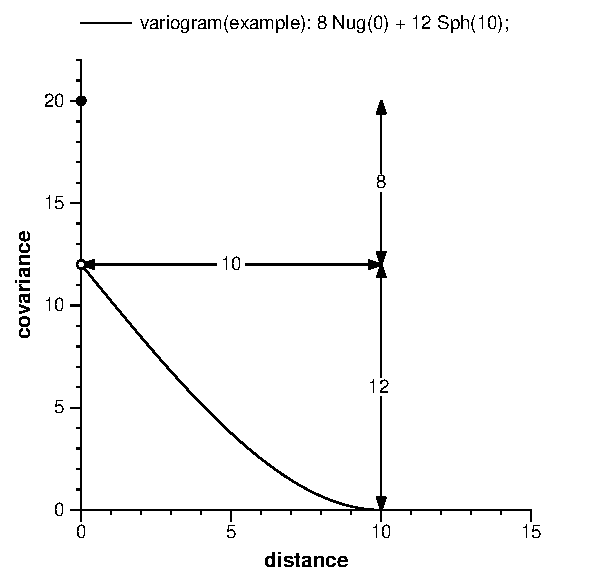
\includegraphics[scale=0.7]{\ext/cov}
\end{center}
\caption {Example variogram {\tt 8 Nug() + 12 Sph(10)}. Semivariance
representation (a) and covariance representation (b)}
\label{fig:example}
\end{figure}

\noindent
Fig.\ \ref{fig:example} gives an example of the variogram model {\tt 8
Nug() + 12 Sph(10)} as semivariance and covariance
representation. Unit models available in gstat are listed in table
\ref{tab:vgm}.

\begin{table}[ht]
\begin{center}
\begin{tabular}{|l|l|l|l|} \hline

{\bf model} & {\bf syntax} & {$\gamma(h)$} & {$h$ range} \\ \hline\hline

% variogram.models.nugget. @SubSubIndex { nugget, {\tt Nug }}
Nugget & \htmladdnormallink{\code{1 Nug(0)}}{png/nug.png}
& 0 & $h = 0$ \\
 & & 1 & $h > 0$ \\ \hline

% variogram.models.spherical. @SubSubIndex { spherical, \code{Sph }}

Spherical & \htmladdnormallink{\code{1 Sph(a)}}{png/sph.png} &
$\frac{3h}{2a}-\frac{1}{2}(\frac{h}{a})^3$ & $0 \le h \le a$ \\
& & $1$ & $h > a$ \\ \hline

% variogram.models.exponential. @SubSubIndex { exponential, \code{Exp}}
Exponential & \htmladdnormallink{\code{1 Exp(a)}}{png/exp.png}
& $1 - \exp(\frac{-h}{a})$ & $h \ge 0$ \\ \hline

% variogram.models.linear. @SubSubIndex { linear, {\tt Lin(0)}}
Linear & \htmladdnormallink{\code{1 Lin(0)}}{png/lin0.png}
& $h$ & $h \ge 0$ \\ \hline

% variogram.models.linears. @SubSubIndex { linear with sill, \code{Lin}}
Linear-with-sill
\footnote{only valid for one-dimensional data}
& \htmladdnormallink{\code{1 Lin(a)}}{png/lina.png}
& $\frac{h}{a}$ & $0 \le h \le a$ \\
 & & $1$ & $h > a$ \\ \hline

% variogram.models.circular. @SubSubIndex { circular, {\tt Cir }}
Circular & \htmladdnormallink{\code{1 Cir(a)}}{png/cir.png} &
$\frac{2 h}{\pi a}\sqrt{1 - (\frac{h}{a})^2}
 + \frac{2}{\pi} \arcsin\frac{h}{a}$
 & $0 \le h \le a$ \\
 & & $1$ & $h > a$ \\ \hline

% variogram.models.pentaspherical. @SubSubIndex { pentaspherical, {\tt Pen }}
Pentaspherical
& \htmladdnormallink{\code{1 Pen(a)}}{png/pen.png} &
$\frac{15h}{8a}- \frac{5}{4}(\frac{h}{a})^3
+\frac{3}{8}(\frac{h}{a})^5$ & $0 \le h \le a$ \\
 & & $1$ & $h > a$ \\ \hline

% variogram.models.Gaussian. @SubSubIndex { Gaussian, {\tt Gau }}
Gaussian & \htmladdnormallink{\code{1 Gau(a)}}{png/gau.png}
 & $\gamma(h) = 1 - \exp(-(\frac{h}{a})^2)$ &
$h \ge 0$ \\ \hline

% variogram.models.Bessel. @SubSubIndex { Bessel, {\tt Bes }}
Bessel
\footnote{$K_1(\cdot)$ is the first order modified Bessel function of the second kind}
& \htmladdnormallink{\code{1 Bes(a)}}{png/bes.png}
 & $1 - \frac{h}{a}{K_1}(\frac{h}{a})$ & $h \ge 0$ \\ \hline

% variogram.models.logarithmic. @SubSubIndex { logarithmic, {\tt Log }}
Logarithmic & \htmladdnormallink{\tt {1 Log(a)}}{png/log.png}
& $0$ & $h = 0$ \\
& & $\log(h + a)$ & $h > 0$ \\ \hline

% variogram.models.power. @SubSubIndex { power, {\tt Pow }}
Power & \htmladdnormallink{\code{1 Pow(a)}}{png/pow.png}
 & $h ^ a $ & $h \ge 0, 0 < a \le 2$ \\ \hline

% variogram.models.periodic. @SubSubIndex { periodic, {\tt Per }}
Periodic & \htmladdnormallink{\code{1 Per(a)}}{png/per.png}
& $1 - \cos(\frac{2\pi h}{a})$ & $h \ge 0$ \\ \hline

\end{tabular}
\end{center}
\caption{Simple variogram models in gstat: the building blocks for a
variogram model\index{variogram!models!table} }
\label{tab:vgm}
\end{table}

\begin{figure}[ht]
\includegraphics[scale=0.38]{\ext/nug}
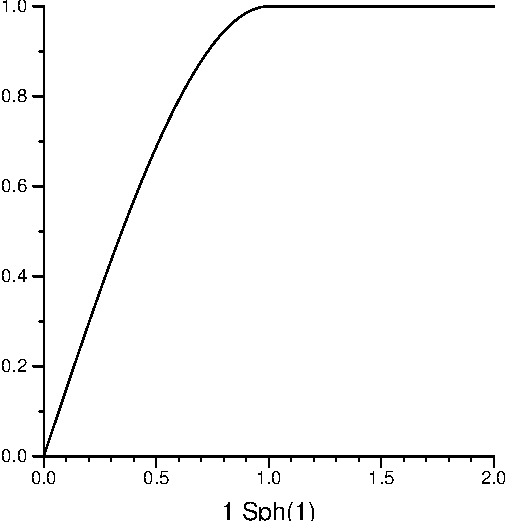
\includegraphics[scale=0.38]{\ext/sph}
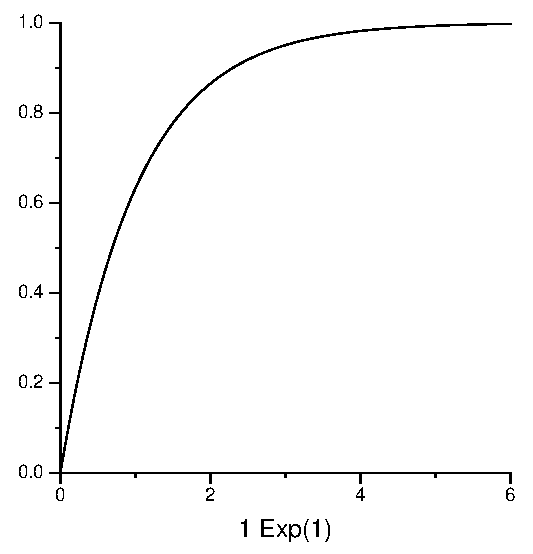
\includegraphics[scale=0.38]{\ext/exp}

\includegraphics[scale=0.38]{\ext/lin}
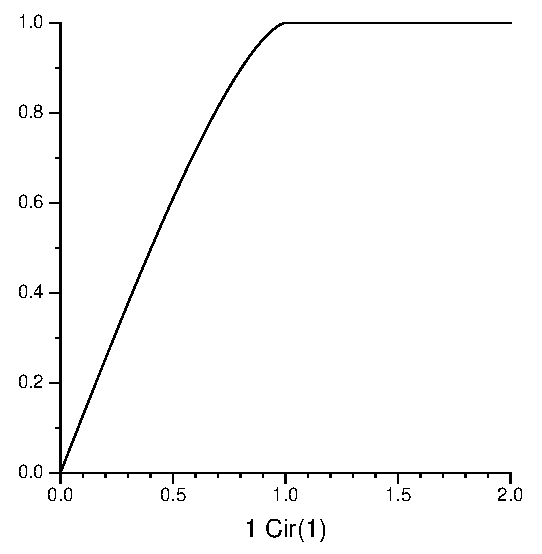
\includegraphics[scale=0.38]{\ext/cir}
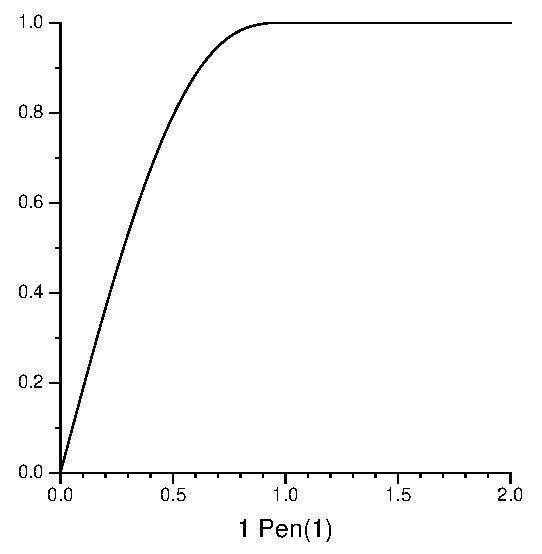
\includegraphics[scale=0.38]{\ext/pen}
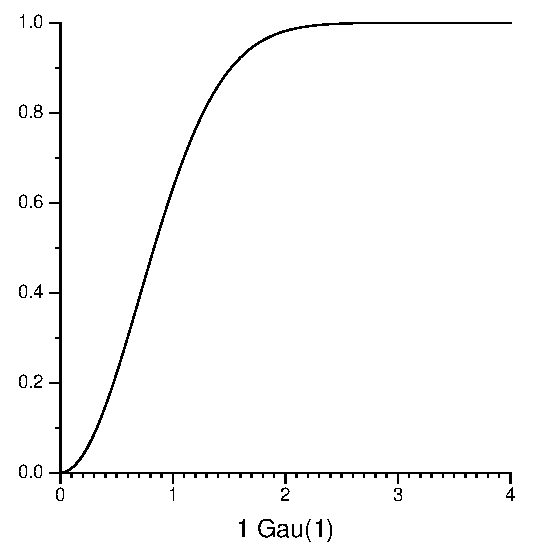
\includegraphics[scale=0.38]{\ext/gau}
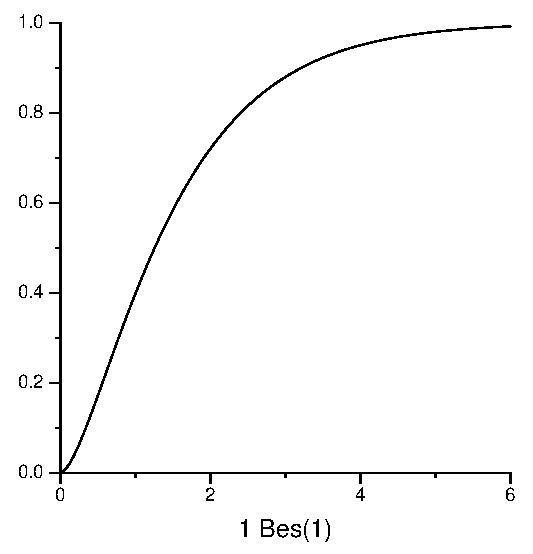
\includegraphics[scale=0.38]{\ext/bes}

\includegraphics[scale=0.38]{\ext/log}
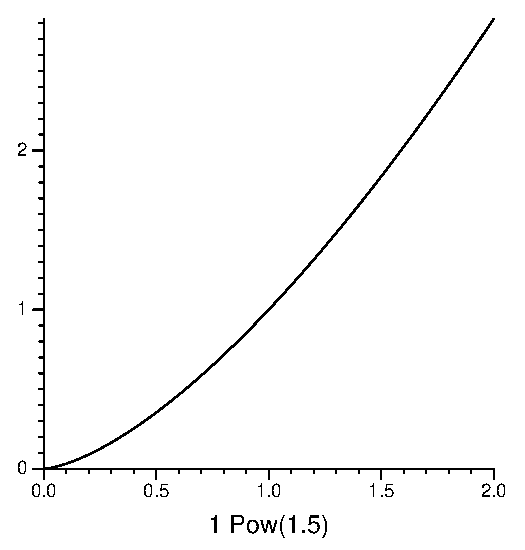
\includegraphics[scale=0.38]{\ext/powa}
\hfill
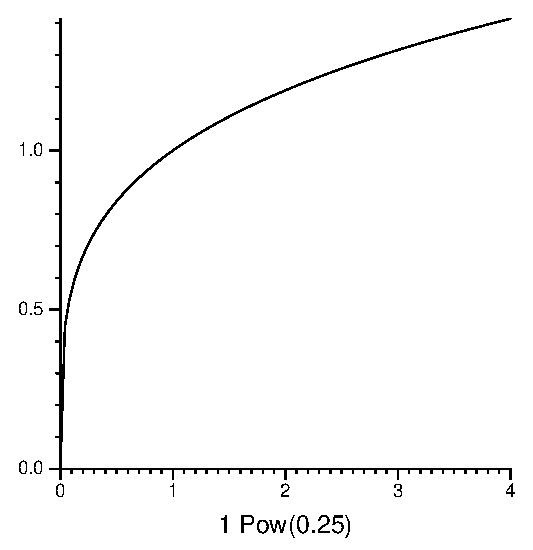
\includegraphics[scale=0.38]{\ext/powb}
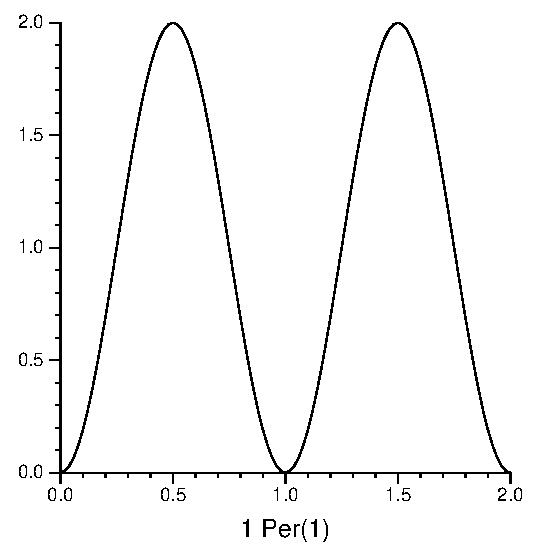
\includegraphics[scale=0.38]{\ext/per}

\caption{The unit basic variogram models
\index{variogram!models!figure}
}
\label{fig:models}
\end{figure}
All unit basic variogram models are shown in Fig.\ \ref{fig:models}.

Note that the {\tt Exp()}, {\tt Gau()} and {\tt Bes()} models reach their
sill asymptotically (as $h \rightarrow \infty$). The `effective range',
is the distance where the variogram reaches 95\% of its maximum, and this
is 3{\tt a} for {\tt Exp(a)}, $\sqrt{3}${\tt a} for {\tt Gau(a)} and 4{\tt
a} for {\tt Bes(a)}. The logarithmic and power model are unbounded (and
are therefore not suitable for covariance modelling or simple kriging).

Pseudo cross variograms may have a non-zero value for $h=0$. An intercept
can be defined as a constant added to the variogram model, e.g.

{\tt 1.5 + 0.5 Nug() + 2.2 Sph(20)}

\noindent
or, equivalently

{\tt 1.5 Int() + 0.5 Nug() + 2.2 Sph(20) }

\noindent
and can be fitted only when a sample variogram estimate is available at
zero distance.

\subsection*{Geometric anisotropy}
\index{variogram!geometric anisotropy}
\index{anisotropy!geometric}

Geometric anisotropy can be modelled for each individual simple model
by addition of two or five anisotropy parameters after the range, e.g.

$c \, Mod(a,p,s)$

\noindent
for 2-d anisotropy, or, for 3-d anisotropy:

$c \, Mod(a,p,q,r,s,t)$

\noindent
Using anisotropy, the variogram model range parameter ($a$) is the
maximum range, that of the major direction of continuity (direction of
spatial correlation at longest distances). The range in the direction
perpendicular to the major direction is the minor range. The anisotropy
ratio is the ratio between the minor range and the major range (a value
between 0 and 1).

A two-dimensional range ellipse is defined by $(a,p,s)$, a
three-dimensional ellipsoid is defined by $(a,p,q,r,s,t)$. In the
two-dimensional case $p$ is the angle for the principal direction of
continuity (measured in degrees, clockwise from positive Y, north),
and $s$ is the anisotropy ratio. So, the range in the major direction
($p$) is $a$, and the range in the minor direction ($p+90$) is $as$.

\begin{figure}[ht]
\begin{center}
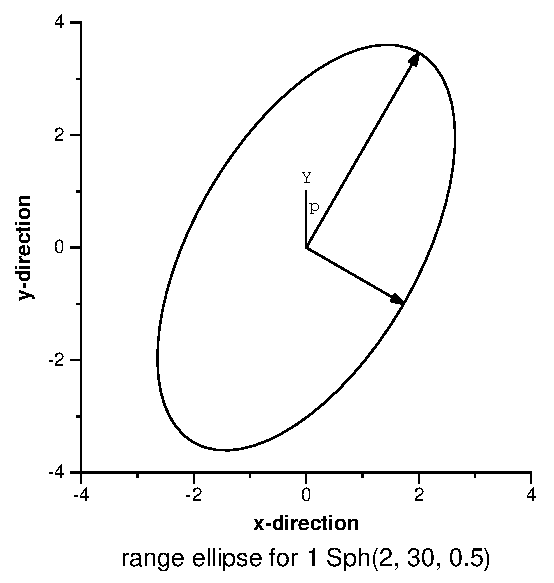
\includegraphics[scale=0.6]{\ext/ell}
\end{center}
\label{fig:ell}
\caption{anisotropy ellipse}
\end{figure}

In three dimensions $p$ is the angle for the principal direction of
continuity (measured in degrees, clockwise from Y, in direction of X),
$q$ is the dip angle for the principal direction of continuity (measured
in positive degrees up from horizontal), $r$ is the third rotation angle
to rotate the two minor directions around the principal direction defined
by $p$ and $q$. A positive angle acts counter-clockwise while looking
in the principal direction. Anisotropy ratios $s$ and $t$ are the ratios
between the major range and each of the two minor ranges. (Note that $c \,
Mod(a,p,s)$ is equivalent to $c \, Mod(a,p,0,0,s,1)$.)

\addtocounter{footnote}{-1}
\footnotetext{only valid for one-dimensional data} \addtocounter{footnote}{1}
\footnotetext{$K_1(\cdot)$ is the first order modified Bessel function of the second kind}

\subsection*{Zonal anisotropy}
\index{variogram!zonal anisotropy}
\index{anisotropy!zonal}

Zonal anisotropy (anisotropy in the sill) can be obtained by defining
geometric anisotropy with large anisotropy ratios. For instance, when
the spatial working domain is not too large (the largest distance in the
area considered does not exceed, let's say, 100), then the model

{\tt 1 Sph(2e5, 90, 1e-5)}

\noindent
will have nearly zero values (and thus be practically absent) in direction
90 (east-west), whereas it will reach the sill (1) at distance 2 in
direction 0 (north-south).

\section{`\thekey{set}'}
\label{sec:set}
\index{set {\em parameter} = {\em value}}

The general form of the {\tt set} command is

{\tt set} {\em parameter} = {\em value} {\tt ;}

\noindent
The list of variables that can be `set' [default value between brackets]:

\Genop
\begin{codelist}

\item[\code{set \thekey{debug}=2;}]
% debug_level @Index {{\tt debug}, set help information level }
set debug level to 2 [1; options are listed in Appendix \ref{app:debug}]

\item[\code{set \theXkey{cn\_max}{cnXmax}=1.0e8;}]
% singularity @Index { singularity check, {\tt set cn\_max}}
check the condition number of matrices. If it is larger than {\tt
cn\_max}, then generate a missing value and report a (near) singularity
warning. Matrices checked are $V$ and $F'V^{-1}F$ (or $F'D^{-1}F$). A
suitable value for {\tt cn\_max} seems $1/ \sqrt{{\tt DBL\_EPSILON}}$,
which is about $10^8$. Condition numbers are estimated using LU
factorization \cite{stewart94}, and may be an order of magnitude
wrong. Condition numbers are reported if {\tt debug} is set to report
covariance matrices. [not set: check for singularity only during variogram
model fitting]

\item[\code{set \thekey{logfile}='gstat.log';}]
% logfile @Index {{\tt logfile}, file name for debug information}
set the file name where debug information is written to (see {\tt set
debug} and Appendix \ref{app:debug}) [stdout, debug information is
written to the screen]

\item[\code{set mv='MisVal';}]
\index{missing value!string, \code{set mv}}
define the default missing value string as {\tt MisVal} [the string
{\tt NA}] (Note that numerical missing values can be defined with
{\tt mv} in a {\tt data} command)

\item[\code{set \thekey{output}='file';}]
\index{output file name@\code{output} file name}
write ascii output to {\tt file} (e.g., variogram estimates,
predictions and variance at non-gridded locations)

\item[\code{set \thekey{plotfile}='file';}]
\index{plotting kriging weights}
{\tt file} defines the file name for gnuplot commands (not set, use
temporary files). When set during ordinary or universal kriging, kriging
weights are written as plot files for gnuplot (see \iskey{plotweights}).
Affects file name usage for variogram plotting through gnuplot.

\item[\code{set \thekey{zero}=1.0e-10;}]
specify the highest value absolote differences in distance and
prediction variances may have to be considered equal to zero [10 $\times$
\verb|DBL_EPSILON|, about $2^{-15}$].

\item[\code{set \thekey{marginals}={\em list};}]
List of values or maps with the mean and variance of the first variable,
the second variable, ... See also section \ref{sec:lhs}.

\end{codelist}

\Vgmop
\begin{codelist}

\item[\code{set \thekey{alpha}=45.0;}]
\index{directional variogram|see{\iskey{alpha}, \iskey{beta}, 
\isXkey{tol\_hor}{tolXhor}, \isXkey{tol\_ver}{tolXver}}}
\index{variogram!directional|see{directional}}
directional sample (co-) variogram: set direction in $<x,y>$ plane, in
positive degrees clockwise from positive y (North) [0.0]

\item[\code{set \thekey{beta}=30.0;}]
directional sample (co-) variogram: set direction in $z$, in positive
degrees up from the $<x,y>$ plane [0.0]

\item[\code{set \thekey{Cressie}=1;}]
\index{robust variogram estimator, \iskey{Cressie}}
\index{variogram!cressie's robust estimator}
(for sample variogram calculation) use Cressie's square-root variogram
estimator [0]

\item[\code{set \thekey{cutoff}=0.5;}]
\index{variogram!cutoff, max. distance}
set cutoff (max. dist. for sample variogram) at 0.5 [a fixed fraction
of the maximum distance, see {\tt set fraction}]

\item[\code{set \thekey{dots}=1000;}]
change the number of plotting points at which gstat will let gnuplot
switch from plotting points (+) with numbers of points of pairs, to
plotting dots without numbers [500]

\item[\code{set \thekey{fit}=1;}]
\index{variogram!modelling!fit method}
fit the variogram model to the experimental variogram, using weighted
least squares fit. Values for \code{fit} are shown in table
\ref{tab:fit} [0, do not fit]

\begin{table}[ht]
\begin{center}
\begin{tabular}{|r|l|c|} \hline
\iskey{fit} & fit by & weight \\ \hline
0 & - & - (no fit) \\
1 & gstat & $N_j$ \\
2 & gstat & $N_j / \{ \gamma(h_j) \}^2$ \\
3 & gnuplot & $N_j$ \\
4 & gnuplot & $N_j / \{ \gamma(h_j) \}^2$ \\
5 & gstat & REML \\ 
6 & gstat & no weights (OLS) \\ 
7 & gstat & ${N_j}/{h_j^2}$ \\ \hline
\end{tabular}
\end{center}
\caption{values for \code{fit}}
\label{tab:fit}
\end{table}

\item[\code{set \theXkey{fit\_limit}{fitXlimit}=1.0e-10;}]
set fit limit to 1.0e-10 (Appendix \ref{app:sample}) [1.0e-6]

\item[\code{set \thekey{format}='\%.3g';}]
the format used for real values in variograms, e.g. {\tt \%.3g} limits
the number of significant digits shown to 3. A valid C-language format
string for a double should be used, misspecification may result in
unpredictable behaviour. [{\tt \%g} : use 6 significant digits]

\item[\code{set \thekey{fraction}=0.25;}]
% set.fraction @SubIndex {{\tt fraction}, for sample variogram }
specify the default cutoff for sample variogram calculation as fraction
of the length of the diagonal in the square or block spanning the data
locations [0.333]

\item[\code{set \thekey{gnuplot}='mygnuplot';}]
invoke the program {\tt mygnuplot} as gnuplot (variogram display)
[gnuplot, or wgnuplot for Win32]

\item[\code{set \thekey{gnuplot35}='gpt35';}]
invoke the program {\tt gpt35} (gnuplot version 3.5) for variogram
display only [use gnuplot, or the value of {\tt set gnuplot}]

\item[\code{set \thekey{gpterm}='latex';}]
\index{gnuplot!output device, \code{gpterm}}
set the gnuplot terminal specification and options (a string to follow
the gnuplot ``set term'' command). This option will overrule the
`postscript' or `gif' settings from the variogram modelling user
interface, thus allowing plotting to other graphic file formats and
modification of options (see gnuplot documentation). [for gif: {\tt 'gif
transparent size 480, 360'}, for {\sc PostScript}: {\tt 'postscript eps
solid 17'}

\item[\code{set \thekey{intervals}=20;}]
\index{variogram!number of intervals, \code{intervals}}
\index{variogram!max distance, \code{intervals}}
specify the default number of intervals for sample variogram
calculation [15]

\item[\code{set \thekey{iter}=20;}]
\index{variogram!modelling!iterations in fitting}
use not more than 20 iterations on iterative fit methods [50]

% \item[\code{set \thekey{jgraph}=1;}]
% write jgraph plot to the file, defined by {\tt set plot} [0, write
% gnuplot plot]

% \item[\code{set \thekey{load}='zinc.sem';}]
% \index{variogram!modelling!loading a sample variogram}
% load a previously calculated sample variogram, instead of calculating it
% from the data. This allows interactive variogram modelling (model fitting)
% using sample variograms that were calculated in batch mode [do not load]
%% NOW obsolete: variogram(x): 'load-file', model;

\item[\code{set \thekey{pager}='less';}]
use `less' as pager to be called from the variogram modeling interface
[the value of the environment variable {\tt PAGER} (if set), or else
the program {\tt more}]

\item[\code{set \thekey{secure}=1;}]
prevent any calls to the functions {\tt system()}, {\tt popen()} or
{\tt remove()}, terminate program whenever one of the first two appear
(once set, it cannot be set back) [0, not secure]

\item[\code{set \thekey{sym}=1;}]
\index{variogram!symmetric or asymmetric}
\index{covariogram!symmetric or asymmetric}
force directional sample cross covariance and pseudo cross semivariance
to be symmetric [0, asymmetric]

\item[\code{set \theXkey{tol\_hor}{tolXhor}=45.0;}]
directional sample (co-)variogram: set horizontal tolerance angle in
degrees [90.0]

\item[\code{set \theXkey{tol\_ver}{tolXver}=20.0;}]
directional sample (co-) variogram: set vertical tolerance angle in
degrees [90.0]

\item[\code{set \thekey{width}=0.05;}]
\index{variogram!interval \code{width}}
set lag width to 0.05 (distance interval width for sample variogram)
[{\tt cutoff/intervals}]

\item[\code{set \thekey{gls}=1;}]
\index{residuals, generalised least squares}
use generalised least squares residuals instead of the default ordinary
least squares (OLS) residuals for sample variograms or covariograms [0,
use OLS or WLS residuals]

\item[\code{set \theXkey{zero\_dist}{zeroXdist}=1;}]
determine what happens with variogram estimates at distance zero. Values
are 1: include in first interval, 2: omit, 3: calculate separately
[1 for variograms, 3 for covariograms]

\end{codelist}

\Prop
\begin{codelist}

\item[\code{set \thekey{idp}=3.5;}]
\index{inverse distance power, \code{idp}}
set inverse distance power to 3.5 [2]

\item[\code{set \thekey{nblockdiscr}=10;}]
\index{block discretization, \code{nblockdiscr}}
use regular block discretization with 10 points in each dimension at
non-zero block size (note: 10 in 3 dimensions results in 1000 discretizing
points) [4, and use Gauss quadrature (see Appendix \ref{app:blocks})]

\item[\code{set \thekey{nsim}=100;}]
\index{simulation!multiple realisations}
\index{multiple realisations}
create 100 independent simulations when following a single random path
(output maps will get the simulation number attached to their names,
therefore short names should be chosen in environments with file name
restrictions) [1]

\item[\code{set \theXkey{n\_uk}{nXuk}=40;}]
(for conditional simulation only) use universal (or ordinary) kriging
instead of simple kriging when the number of data in a kriging setting
is greater than or equal to 40. For multivariable prediction the
neighbourhood size is summed over all variables, otherwise it is evaluated
per variable. Setting {\tt n\_uk} to zero limits use of simple kriging
to empty neighbourhoods only [very large: always use simple kriging]

\item[\code{set \thekey{order}=2;}]
define the action when order relation violations occur during indicator
simulation (section \ref{sec:simulation}; table \ref{tab:orvc}) or
indicator kriging (section \ref{sec:prediction}). Values are 0: no
correction for indicator kriging, assure that estimated probabilities
are in [0,1] before simulation; 1: as 0, but also for indicator kriging;
2: rescale the estimated probabilities if their sum is larger than 1; 3:
rescale the estimated probabilities so that they sum up to 1; 4: do
order relation correction for cumulative indicators (using the
upward-downward averaging steps of GSLIB \cite{deutsch92}). [0: do
only basic order relation violation corrections for indicator
simulation]

\item[\code{set \thekey{plotweights}=10;}]
\index{\code{plotting kriging weights}}
When \iskey{plotfile} is set, kriging weights will be plotted during
ordinary or universal kriging. If \code{plotweights} is larger than
1, data point sizes are proportional to kriging weights using size
intervals of $\frac{1}{\mbox{\code{plotweights}}}$. If not (default),
kriging weights are plotted as data point labels (i.e., as text).

\item[\code{set \thekey{quantile}=0.25;}]
\index{local quantile estimation}
\index{quantile estimation}
when {\tt method} was set to {\tt med}, report $p$-quantile of local
neighbourhood selection as prediction value, and $(1-p)$-value as
prediction variance [0.5: the median]

\item[\code{set \thekey{rp}=0;}]
\index{random path, \code{rp}}
follow regular, non-random path during sequential simulation [1, follow
a random path]

\item[\code{set \thekey{seed}=1023;}]
\index{random number \code{seed}, \code{useed}}
set seed for random number generator [0: seed is read from the internal
clock. If possible, microseconds are used. To check this, run gstat a
few times with \iskey{debug} set to 2].

\item[\code{set \thekey{useed}=4053341103U;}]
set seed for random number generator when outside the range of a signed
integer; note the `U' at the end of the number [see \code{seed}].

\item[\code{set \thekey{sparse}=10;}]
Use sparse matrix routines for covariance matrix. The number of {\tt
sparse} should be a reasonable estimate of the number of non-zero columns
in each row of the covariance matrix $V$. [only available when sparse
matrix routines in meschach are linked in; 0: use dense matrices]

\item[\code{set \thekey{xvalid}=1;}]
\index{cross validation, \iskey{xvalid}}
turn cross validation on (if prediction is possible) [0, no cross
validation]

\item[\code{set \thekey{zmap}=10.0;}]
\index{height of mask map}
set height of mask map(s) to 10 when observations are 3-D. [0.0]

\item[\code{set \thekey{lhs}=1;}]
\index{Latin hypercube sampling}
Apply Latin hypercube sampling to Gaussian simulations; see also
\iskey{marginals}

\item[\code{set \thekey{nocheck}=1;}]
Ignore error in case of an non-permitted coregionalisation (intrinsic
correlation or linear model of coregionalisation)

\end{codelist}

\section{`\thekey{method}'}
\label{sec:method}
\index{prediction!method}

Values for {\tt method} that make gstat deviate from the default
action are:

% method. @Index {{\tt method }

\begin{codelist}
\item[\code{\thekey{gs}}]
\index{simulation!Gaussian, \iskey{gs}}
\index{Gaussian simulation, \iskey{gs}}
override the default kriging method to get Gaussian simulations
(section \ref{sec:simulation})

\item[\code{\thekey{is}}]
\index{simulation!indicator, \iskey{is}}
override the default kriging method to get indicator simulations
(section \ref{sec:simulation})

\item[\code{\thekey{semivariogram}}]
\index{variogram!sample}
\index{sample variogram}
sample semivariance on output (see also \iskey{fit}, section
\ref{sec:set})

\item[\code{\thekey{covariogram}}]
\index{covariogram!sample}
\index{sample covariogram}
sample covariogram on output

\item[\code{\thekey{trend}}]
\index{trend!estimation}
spatial trend estimation ($x_0 \hat \beta$), using generalised least
squares if variograms are specified, or else using ordinary or weighted
least squares (see Appendix \ref{app:eqs})

\item[\code{\thekey{map}}]
\index{map values at data locations}
report the value of $m$ mask maps at the prediction location of
{\tt data()} as the output values, provided that $n$ (dummy) input
variable are defined, with $n \ge m/2$ (\ex{9})

\item[\code{\thekey{distance}}]
\index{distance to prediction locations}
report distance to nearest observation as the predicted value, and the
distance to the most distant observation (in the neighbourhood
selection, if defined) as prediction variance

\item[\code{\thekey{nr}}]
\index{neighbourhood!size as prediction value \iskey{nr}}
report number of observations in neighbourhood as predicted value, and,
if omax was set, the number of non-empty octants (or quadrants) as
prediction variance

\item[\code{\thekey{div}}]
\index{local diversity, \code{div}}
diversity (the number of distinct values) in a local neighbourhood is
reported as the predicted value, the modus of the values (the value that
occurred most often in a local neighbourhood) is reported as prediction
variance

\item[\code{\thekey{med}}]
local median or quantile estimation, see \iskey{quantile} in
section \ref{sec:set}; for minimum and maximum values in each local
neighbourhood, set \iskey{quantile} to 0.0.

\item[\code{\thekey{skew}}]
report skewness as predicted value, and kurtosis as the prediction
variance value for values in a local neighbourhood. Uses
methods-of-moments estimators: 
${\mbox Sk}=\frac{1}{\sigma^3 n}\sum_{i=1}^n (y_i - \mu)^3$
${\mbox K}=\frac{1}{\sigma^4 n}\sum_{i=1}^n (y_i - \mu)^4$

\item[\code{\thekey{point-in-polygon}}]
Provided a set of (closed) polygons is given with the \iskey{edges}
command, the (first) polygon in which the prediction location is located
is given in the output. Predicted value carries the file number of the
polygon, prediction variance the polygon number in the file.  See also
Appendix \ref{app:edges}

\end{codelist}

\chapter{Further control}
\label{ch:environment}

\section{Start-up}
\label{sec:start}
\index{start up files}

% gstatrc. @Index {{\tt GSTATRC environment variable}}
% home.gstatrc. @Index {{\tt "$HOME/.gstatrc"}}

When gstat is started, it first looks for an initialization file to
load. If the environment variable {\tt GSTATRC} specifies a file name,
gstat will read the contents of this file, or else gstat will search for
the file \verb|$HOME/.gstatrc| and read it when found. If present, the
initialization file should contain valid gstat commands. After reading
the initialization file, command line options are processed, and finally
the command file is processed. The processing order determines when
previously set commands will be overridden.

Information on gnuplot customization is obtained by starting gnuplot and
typing ``help'' or ``help environment''. (If the help file is not found,
the environment variable {\tt GNUHELP} should be set to the gnuplot help
file, {\tt gnuplot.gih}.)

\section{Command line options}
\label{sec:clo}
\index{command line options}

Some options in gstat can be specified on the command line. Command line
options appear between the gstat command and the command file name,
options start with a {\tt -}, and option arguments follow the option
letter, possible separated by white space, e.g. the command line

{\tt gstat -l gstat.log -d 2 zinc.gst }

\noindent
has two options, `{\tt l}' having argument {\tt gstat.log} and `{\tt
d}' having argument {\tt 2}. The final argument, {\tt zinc.gst} is not
part of an option, it is the main argument (the command file). A short
list of command line options is obtained by typing

{\tt gstat -h}

\noindent Special file names (pipes, append files) are explained
in section \ref{sec:filen}. The list of options is given in table
\ref{tab:clo}.

% command.line. @Index {command line options}

\begin{table}
\begin{tabular}[h]{|l|p{9cm}|l|} \hline
option & {\em meaning} & {\em keyword}\\ \hline
{\tt -C} & print copyright notice & \\
{\tt -W} & print no-warranty notice  & \\
{\tt -v} & print long version information & \\
{\tt -i} & enter the interactive variogram modeling user interface
(only available when \iskey{method} was not set previously) & \\
{{\tt -d} {\em n}} & invoke debug level {\em n}, see table \ref{tab:debug} & \iskey{debug} \\
{\tt -s} & silent mode: print only warnings and errors & \iskey{debug} \\
{\tt -o file} & specify (ascii) output file & \iskey{output}\\
{\tt -p file} & specify gnuplot plot file & \iskey{plotfile} \\
{\tt -l file} & specify (ascii) log file for debug
information (default to screen) & \iskey{logfile} \\
{\tt -S} & secure mode & \iskey{secure}\\
{{\tt -e} {\em action}} & execute action {\em action} (see
section \ref{sec:actions}) & \\ \hline
\end{tabular}
\caption{command line options}
\label{tab:clo}
\end{table}

\section{Random number generators}
\label{sec:rng}
\index{random number generators}

For the simulation of random fields, gstat can use one of several random
number generators (RNG). The default generator depends on the platform
on which gstat was compiled:
\begin{itemize}
\item when gstat is used as a package from R or library from S, the
R or S random number generator is used;
\item for gstat stand alone, 
when the GNU Scientific Library (GSL) was present, the default
rng is mt19937 in this library
\item else, Marsaglia's random number generator is used.
\end{itemize}

From within R or S-PLUS, , and {\tt set.seed()} can be used to control
the seed. For stand-alone gstat, the seed of the RNG can be set by the
variable \iskey{seed}. Default, the seed is read from the CPU clock
(using microseconds, when the function {\tt gettimeofday} is present,
or else seconds). 

The GSL provides 26 different generators, and the one used is controlled
by setting the environment variable GSL\_RNG\_TYPE to one of the following
values: {\tt ranlux389 ranlux cmrg mrg mt19937 tt800 taus ran0 ran1
ran2 ran3 ranf rand48 ranmar zuf slatec r250 random minstd uni uni32 vax
transputer rand random8 randu}. See the GSL documentation for details.
The environment variable GSL\_RNG\_SEED may be used to override the seed
of gstat (set or default).

\section{Special file names}
\label{sec:filen}
\index{special file names}
\index{temporary files}
\index{pipes}

Certain special file names are allowed in gstat. They enable filtering,
appending to files, using standard input or output streams and command
output substitution. (They will not have this effect for PCRaster
file names.)

\begin{codelist}
\item[\code{'> file'}]
If \code{file} exists, then append the output to \code{file} (if it is
an output file) instead of starting with a fresh file

\item[\code{'| file'}]
Open \code{file} as a pipe, either for reading or for writing

\item[\code{'-'}]
Use, instead of a disk file, for a reading process the stream
\code{stdin}, or for a writing process the file \code{stdout}

\item[\code{`cmd`}]
execute the shell command \code{cmd} and substitute its output for the
file name

\end{codelist}

Using pipes is at the user's responsibility. Blindly executing command
files that contain file names with pipes to harmful commands may result
in damage (loss of files for instance). This also applies to the setting
of the {\tt gnuplot} command(s), see section \ref{sec:set}. Potential
damage from such situations is considered as ``consumers risk'', it is
comparable to renaming harmful programs to often-used commands.

For safety reasons, the variable \iskey{secure} can be set to 1, which
prohibits gstat from system calls, creating pipes or deleting temporary
files. Unlike other variables, once \iskey{secure} is set, it cannot be
set back (indeed, for security).

As an example of using a pipe as file name, the first variable in
\ex{12} containing the data selection from {\tt zinc\_map.eas} with
a zero in column 5, could have been defined directly in terms of {\tt
zinc\_map.eas} as

\index{awk}
\begin{verbatim}
data(zinc.at.0):
"| awk '{if(NR<11||$5==0){print $0}}' zinc_map.eas",
 x=1, y=2, v=3, log, min = 20, max = 40, radius = 1000;
\end{verbatim}

\noindent
provided that the {\tt awk} program is available.

\section{Execute ({\tt -e}) actions}
\label{sec:actions}
\index{actions}

Several simple ``special actions'' are available in (``linked into'')
gstat. They are invoked as

{\tt gstat -e} {\em action arguments}

\noindent
and are strictly controlled by command line options and arguments. A
list of available {\em action}s is obtained by calling

{\tt gstat -e}

\noindent
and usage for each {\em action} is printed after running

{\tt gstat -e} {\em action}

\noindent
without arguments. Following is a list of available {\em actions}:

\begin{codelist}
\item[\code{\thekey{cover}} \rmit{out\_map in\_map1 in\_map2 ...}]
cover several input maps into the output map: substitute in
\rmit{out\_map} the missing values of {\em in\_map1} with the first
non-missing value found in subsequent input maps, on a cell-by-cell basis

\item[\code{\thekey{convert}}]
Converts grid map file from one format to another (minimal converter)

\item[\code{\thekey{nominal}} \rmit{out\_map in\_map0 in\_map1 ... in\_mapn}]
from multiple input grid map files write in each grid cell of
\rmit{out\_map} the number of the first map with a non-zero value in
that grid cell (a value in $[0,...,n]$)

\item[\code{\thekey{map2fig}}] convert point data or grid map data to fig
(XFig/fig2dev) file. XFig is a vector graphics editor for X-Windows that
supports exporting to numerous formats.

\item[\code{\thekey{map2gif}}] convert grid map file to
gif file. The gif library used to generate gif's from
maps is not distributed as part of the gstat distribution;
see \htmladdnormallink{\code{http://www.boutell.com/gd/}}
{http://www.boutell.com/gd/}

\item[\code{\thekey{map2png}}] 
See \iskey{map2gif}. Modern versions of the gd library only support PNG
instead of GIF, because of the unisys license thing. If such a version
of gd is found, gstat only supports map2png to create PNG's.

\item[\code{\iskey{semivariogram}}]
calculate sample variogram, using command line interface

\item[\code{\iskey{covariogram}}]
calculate sample covariogram, using command line interface

\item[\code{\thekey{semivariance}}]
print semivariance table for a variogram model

\item[\code{\thekey{covariance}}]
print covariance table for a variogram model

\item[\code{\thekey{statistics}}]
output summary statistics for values read from one or more files (for
each file: min, max, median, quantiles, mean, standard deviation, n)

\end{codelist}

\section{Compiling and installing gstat}
\label{sec:compiling}

In order to work with gstat, binary executables of gstat and gnuplot are
needed. Both programs can be obtained in source form from the internet
and they can be compiled to executables using an {\sc ansi-c} compiler. On
Unix systems, typing in the gstat directory

\code{./configure}
\index{configure}

\noindent
followed by

\code{make; make install }
\index{installing!gstat}

\noindent
may be sufficient for compiling and installing gstat.

Similarly, for compiling gnuplot, typing

\code{./configure; make; make install}

\noindent
in the gnuplot directory may be sufficient to compile an install
gnuplot. Type

\code{./configure --help }
\index{installing!gnuplot}

\noindent
to obtain the command line options for non-default configuring (e.g. of
install directories, libraries used). By default, for compatibility
reasons the output files from flex and bison are used for compiling
gstat. If you want to use your own lex or yacc version, remove the files
lex.c, parse.c and parse.h from the src directory. From bash or ksh,
this is also accomplished by:

\code{LEXYACC=1 ./configure}

To my knowledge gstat has been successfully compiled on HP-UX,
IBM AIX, Dec OSF/Alpha, SunOS, SGI, Linux, MS-Windows (95, NT) and
MS-DOS/DPMI. When modifications to the makefiles or source files are
necessary to make the software run, please report them to \gstatinfo

\index{library!csf}
\index{library!meschach}
\index{library!gd}
\index{meschach matrix library}

Gstat requires two external libraries: the Meschach matrix
library \cite{stewart94} (available from netlib) and PCRaster
grid map API (csf, version 2). Both are distributed as
part of the gstat source code distribution.  One other
library is optional, and required for \iskey{map2gif}: the
\htmladdnormallink{gd}{http://www.boutell.com/gd/index.html} gif library
(copyright 1994, 1995, Quest Protein Database Center, Cold Spring Harbor
Labs, see \code{http://www.boutell.com/gd/index.html}).

Binary executable files should be installed in a directory in the search
path for executables.

\chapter{Example command files}
\label{ch:examples}
\index{example command files}

\begin{figure}
(a) 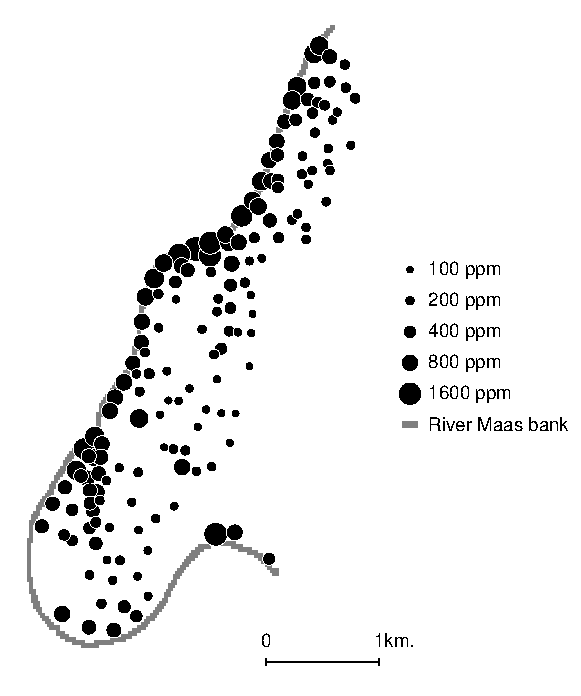
\includegraphics[width=0.45\textwidth]{\ext/zn_map} 
(b) 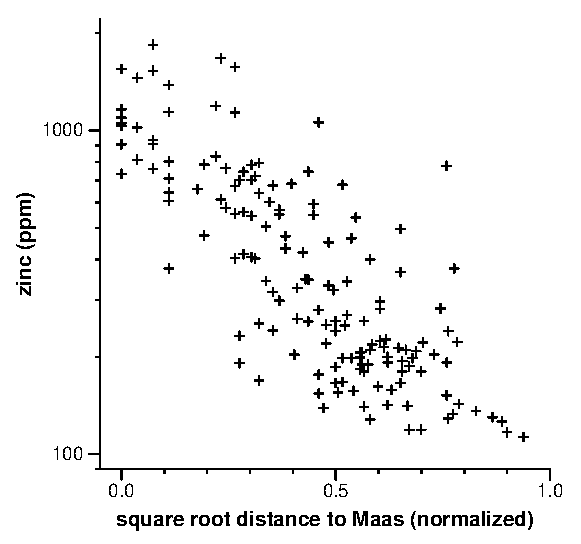
\includegraphics[width=0.45\textwidth]{\ext/scat} 
\vspace*{.7cm}
(c) 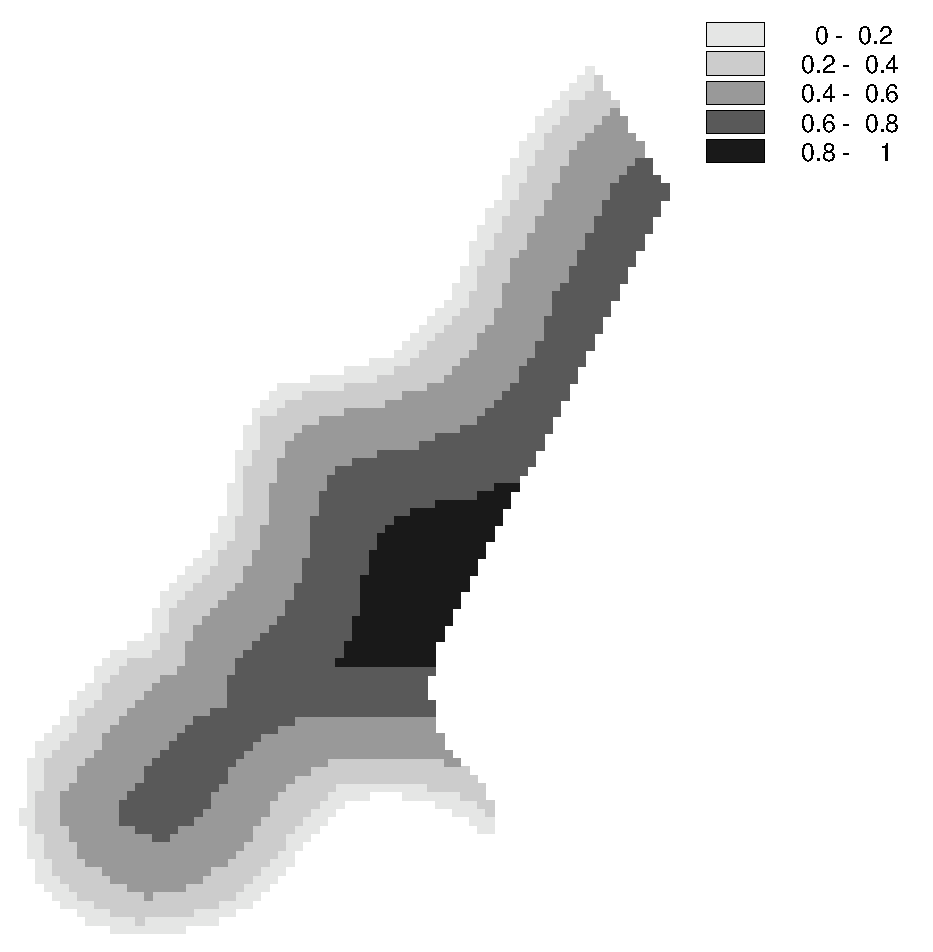
\includegraphics[width=0.45\textwidth]{\ext/sqrtdist} 
(d) 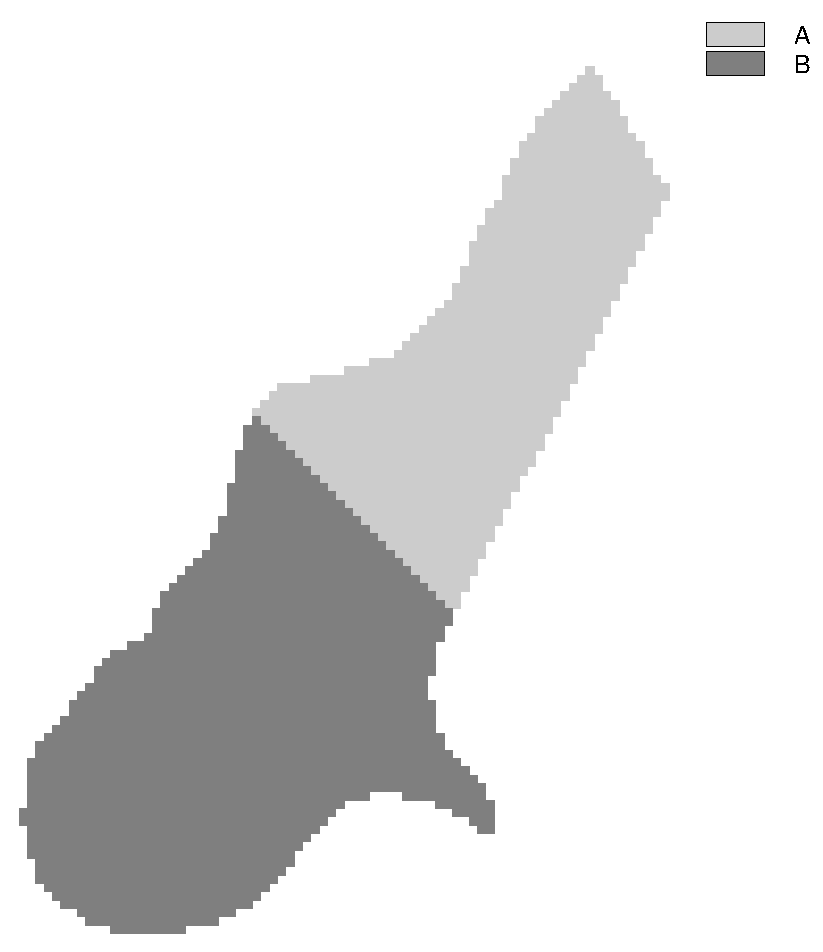
\includegraphics[width=0.45\textwidth]{\ext/part} 

\caption {
 (a) map of zinc measurements in the top soil,
 (b) scatter plot of zinc measurements and distance to the river Maas,
 (c) map with normalised square root distance to the river Maas,
 (d) partitioning of the prediction area }
\label{fig:zinc}
\end{figure}

Following are the example command files, as distributed with gstat. The
data (\htmladdnormallink{zinc concentrations of the top soil}
{png/zn_map.png}, Fig.\ \ref{fig:zinc}a) are collected
in a flood plain of the river Maas, not far from where the Maas
entered the Netherlands (Borgharen, Itteren, about 3 to 5 km North of
Maastricht). All coordinates are in metres, using the standard coordinates
of Dutch topographical maps. Moving from the river, zinc concentrations
\htmladdnormallink{tend to decrease}{png/scat.png}(Fig.  \ref{fig:zinc}b).

For the universal kriging examples, let the function $D(x)$ be the
function that is for every location $x$ the (normalised) square
root distance to the river. This function is physically stored
for the observation locations in column 4 of {\tt zinc\_map.eas}
(as obtained in \ex{9}), and for the prediction locations in
the map \htmladdnormallink{{\tt sqrtdist.map}}{png/sqrtdist.png}
(Fig.\ \ref{fig:zinc}c). The prediction area is split in two
separate sub-regions, $A$ and $B$ (Fig.\ \ref{fig:zinc}d). Let
the function $I_A (x)$ be 1 if $x \in A$ or else 0; and let the function
$I_B (x)$ be 1 if $x \in B$ or else 0.

The functions $I_A (x)$ and $I_B (x)$ are physically stored for the
observation locations in columns 5 and 6 of \htmladdnormallink{{\tt
zinc\_map.eas}}{zinc_map.html}, and for the prediction locations in
the maps \htmladdnormallink{{\tt part\_a.map}}{png/part_a.png} and
\htmladdnormallink{{\tt part\_b.map}}{png/part_b.png}. (Note that the
partitioning in $A$ and $B$ is arbitrary, it serves only illustrational
purposes.)

The following command files, data and maps are distributed with gstat.

These command files are purely for illustration and as such only suggest
possible forms of analysis. Remind that everything from a \code{\#}
to the end of the line is comment.

\newpage

% DO NOT EDIT--Automatically generated from example.in
\section{Example 1. Variogram modelling }
\label{ex:1}
{\tt \#} {\em {}}\\
{\tt \#} {\em One variable definition: {}}\\
{\tt \#} {\em to start the variogram modelling user interface. {}}\\
{\tt \#} {\em {}}\\
{\tt data(zinc): '\htmladdnormallink{zinc.eas}{http://www.geog.uu.nl/gstat/manual/zinc.html}', \iskey{x}=1, \iskey{y}=2, \iskey{v}=3; {}}\\
\section{Example 2. Variogram modelling of two variables }
\label{ex:2}
{\tt \#} {\em {}}\\
{\tt \#} {\em Two variables with (initial estimates of) variograms, {}}\\
{\tt \#} {\em start the variogram modelling user interface {}}\\
{\tt \#} {\em {}}\\
{\tt data(zinc): '\htmladdnormallink{zinc.eas}{http://www.geog.uu.nl/gstat/manual/zinc.html}', \iskey{x}=1, \iskey{y}=2, \iskey{v}=3;   {}}\\
{\tt data(ln\_zinc): '\htmladdnormallink{zinc.eas}{http://www.geog.uu.nl/gstat/manual/zinc.html}', \iskey{x}=1, \iskey{y}=2, \iskey{v}=3, \iskey{log}; {}}\\
{\tt  {}}\\
{\tt variogram(zinc): 10000 Nug() + 140000 Sph(800); {}}\\
{\tt variogram(ln\_zinc): 1 Nug() + 1 Sph(800); {}}\\
\section{Example 3. Inverse distance interpolation }
\label{ex:3}
{\tt \#} {\em {}}\\
{\tt \#} {\em Inverse distance interpolation on a mask map {}}\\
{\tt \#} {\em {}}\\
{\tt data(zinc): '\htmladdnormallink{zinc.eas}{http://www.geog.uu.nl/gstat/manual/zinc.html}', \iskey{x}=1, \iskey{y}=2, \iskey{v}=3; {}}\\
{\tt mask:       '\htmladdnormallink{mask\_map}{http://www.geog.uu.nl/gstat/manual/gif/mask_map.gif}.tif';     \#} {\em the prediction locations {}}\\
{\tt predictions(zinc): '\htmladdnormallink{id\_pr}{http://www.geog.uu.nl/gstat/manual/gif/id_pr.gif}'; \#} {\em result map {}}\\
\section{Example 4. Ordinary block kriging}
\label{ex:4}
{\tt \#} {\em {}}\\
{\tt \#} {\em Local ordinary block kriging at non-gridded locations {}}\\
{\tt \#} {\em {}}\\
{\tt data(zinc): '\htmladdnormallink{zinc.eas}{http://www.geog.uu.nl/gstat/manual/zinc.html}', \iskey{x}=1, \iskey{y}=2, \iskey{v}=3,  {}}\\
{\tt   \iskey{min}=20, \iskey{max}=40, \iskey{radius}=1000; \#} {\em local neighbourhood {}}\\
{\tt variogram(zinc): 2.42e+04 Nug(0) + 1.34e+05 Sph(800); {}}\\
{\tt data(): '\htmladdnormallink{locs.eas}{http://www.geog.uu.nl/gstat/manual/locs.html}', \iskey{x}=1, \iskey{y}=2; \#} {\em prediction locations {}}\\
{\tt blocksize: dx=40, dy=40;      \#} {\em 40 $\times$ 40 block averages {}}\\
{\tt set \iskey{output} = '\htmladdnormallink{zincok.out}{http://www.geog.uu.nl/gstat/manual/zincok.html}';    \#} {\em ascii output file {}}\\
\section{Example 5. Simple kriging on a mask map }
\label{ex:5}
{\tt \#} {\em {}}\\
{\tt \#} {\em Local simple point kriging on a mask map {}}\\
{\tt \#} {\em {}}\\
{\tt data(ln\_zinc): '\htmladdnormallink{zinc.eas}{http://www.geog.uu.nl/gstat/manual/zinc.html}', \iskey{x}=1, \iskey{y}=2, \iskey{v}=3, \iskey{log},  {}}\\
{\tt   \iskey{min}=20, \iskey{max}=40, \iskey{radius}=1000, \isXkey{sk\_mean}{skXmean}=5.9; {}}\\
{\tt variogram(ln\_zinc): 0.0554 Nug(0) + 0.581 Sph(900); {}}\\
{\tt mask:                 '\htmladdnormallink{mask\_map}{http://www.geog.uu.nl/gstat/manual/gif/mask_map.gif}.tif'; {}}\\
{\tt predictions(ln\_zinc): '\htmladdnormallink{lzn\_skpr}{http://www.geog.uu.nl/gstat/manual/gif/lzn_skpr.gif}'; {}}\\
{\tt variances(ln\_zinc):   '\htmladdnormallink{lzn\_skvr}{http://www.geog.uu.nl/gstat/manual/gif/lzn_skvr.gif}'; {}}\\
\section{Example 6. Unconditional simulation }
\label{ex:6}
{\tt \#} {\em {}}\\
{\tt \#} {\em Unconditional Gaussian simulation on a mask {}}\\
{\tt \#} {\em (local neigbourhoods, simple kriging) {}}\\
{\tt \#} {\em {}}\\
{\tt \#} {\em defines empty variable: {}}\\
{\tt data(ln\_zn\_dummy): dummy, \isXkey{sk\_mean}{skXmean}=5.9, \iskey{max}=20; {}}\\
{\tt variogram(ln\_zn\_dummy): 0.0554 Nug(0) + 0.581 Sph(900); {}}\\
{\tt mask:  '\htmladdnormallink{mask\_map}{http://www.geog.uu.nl/gstat/manual/gif/mask_map.gif}.tif'; {}}\\
{\tt method:  gs; \#} {\em Gaussian simulation instead of kriging {}}\\
{\tt predictions(ln\_zn\_dummy): '\htmladdnormallink{lzn\_uspr}{http://www.geog.uu.nl/gstat/manual/gif/lzn_uspr.gif}'; {}}\\
{\tt set nsim = 10; {}}\\
\section{Example 7. Conditional simulation }
\label{ex:7}
{\tt \#} {\em {}}\\
{\tt \#} {\em Gaussian simulation, conditional upon data {}}\\
{\tt \#} {\em (local neighbourhoods, simple and ordinary kriging) {}}\\
{\tt \#} {\em {}}\\
{\tt data(ln\_zinc): '\htmladdnormallink{zinc.eas}{http://www.geog.uu.nl/gstat/manual/zinc.html}', \iskey{x}=1, \iskey{y}=2, \iskey{v}=3, \iskey{log}, {}}\\
{\tt   \isXkey{sk\_mean}{skXmean}=5.9, \iskey{max}=20; {}}\\
{\tt variogram(ln\_zinc): 0.0554 Nug(0) + 0.581 Sph(900); {}}\\
{\tt mask: '\htmladdnormallink{mask\_map}{http://www.geog.uu.nl/gstat/manual/gif/mask_map.gif}.tif'; {}}\\
{\tt method: gs; {}}\\
{\tt predictions(ln\_zinc): '\htmladdnormallink{lzn\_cspr}{http://www.geog.uu.nl/gstat/manual/gif/lzn_cspr.gif}'; {}}\\
{\tt set nsim=10; {}}\\
\section{Example 8. Ordinary block kriging on a mask map }
\label{ex:8}
{\tt \#} {\em {}}\\
{\tt \#} {\em Change of support: local ordinary block kriging on a mask {}}\\
{\tt \#} {\em {}}\\
{\tt data(ln\_zinc): '\htmladdnormallink{zinc.eas}{http://www.geog.uu.nl/gstat/manual/zinc.html}', \iskey{x}=1, \iskey{y}=2, \iskey{v}=3, \iskey{log}, {}}\\
{\tt   \iskey{min}=20, \iskey{max}=40, \iskey{radius}=1000; {}}\\
{\tt variogram(ln\_zinc): 0.0554 Nug(0) + 0.581 Sph(900); {}}\\
{\tt mask: '\htmladdnormallink{mask\_map}{http://www.geog.uu.nl/gstat/manual/gif/mask_map.gif}.tif'; {}}\\
{\tt predictions(ln\_zinc): '\htmladdnormallink{lzn\_okbp}{http://www.geog.uu.nl/gstat/manual/gif/lzn_okbp.gif}'; {}}\\
{\tt variances(ln\_zinc):   '\htmladdnormallink{lzn\_okbv}{http://www.geog.uu.nl/gstat/manual/gif/lzn_okbv.gif}'; {}}\\
{\tt blocksize: dx=40, dy=40; \#} {\em define block dimensions {}}\\
\section{Example 9. Map values at point locations }
\label{ex:9}
{\tt \#} {\em {}}\\
{\tt \#} {\em Obtain map values at data() locations {}}\\
{\tt \#} {\em (Point-map overlay) {}}\\
{\tt \#} {\em {}}\\
{\tt data(a): \iskey{dummy}; \#} {\em define n dummy data variable (n=n\_masks/2) {}}\\
{\tt data(b): \iskey{dummy};  {}}\\
{\tt data(): '\htmladdnormallink{zinc.eas}{http://www.geog.uu.nl/gstat/manual/zinc.html}', \iskey{x}=1, \iskey{y}=2, \iskey{v}=3; \#} {\em prediction locations {}}\\
{\tt method: map;                       \#} {\em mapvalues as `predictions' {}}\\
{\tt masks: '\htmladdnormallink{sqrtdist}{http://www.geog.uu.nl/gstat/manual/gif/sqrtdist.gif}', '\htmladdnormallink{part\_a}{http://www.geog.uu.nl/gstat/manual/gif/part_a.gif}', '\htmladdnormallink{part\_b}{http://www.geog.uu.nl/gstat/manual/gif/part_b.gif}'; \#} {\em the maps {}}\\
{\tt set \iskey{output} = '\htmladdnormallink{zincmap.eas}{http://www.geog.uu.nl/gstat/manual/zincmap.html}';        \#} {\em ascii output file. {}}\\
\section{Example 10. Multiple kriging }
\label{ex:10}
{\tt \#} {\em {}}\\
{\tt \#} {\em Multiple kriging: prediction on more than one variable {}}\\
{\tt \#} {\em (ordinary kriging of two variables) {}}\\
{\tt \#} {\em (note that zinc\_map.eas wass obtained through ex09.gst) {}}\\
{\tt \#} {\em {}}\\
{\tt data(ln\_zinc): '\htmladdnormallink{zincmap.eas}{http://www.geog.uu.nl/gstat/manual/zincmap.html}', \iskey{x}=1, \iskey{y}=2, \iskey{v}=3, \iskey{log}, {}}\\
{\tt   \iskey{min}=20, \iskey{max}=40, \iskey{radius}=1000; {}}\\
{\tt data(sq\_dist): '\htmladdnormallink{zincmap.eas}{http://www.geog.uu.nl/gstat/manual/zincmap.html}', \iskey{x}=1, \iskey{y}=2, \iskey{v}=4, {}}\\
{\tt   \iskey{min}=20, \iskey{max}=40, \iskey{radius}=1000; {}}\\
{\tt variogram(ln\_zinc): 0.0554 Nug(0) + 0.581 Sph(900); {}}\\
{\tt variogram(sq\_dist): 0.0631 Sph(900); {}}\\
{\tt mask: '\htmladdnormallink{mask\_map}{http://www.geog.uu.nl/gstat/manual/gif/mask_map.gif}.tif'; {}}\\
{\tt predictions(ln\_zinc): '\htmladdnormallink{lzn\_okpr}{http://www.geog.uu.nl/gstat/manual/gif/lzn_okpr.gif}'; {}}\\
{\tt variances(ln\_zinc):   '\htmladdnormallink{lzn\_okvr}{http://www.geog.uu.nl/gstat/manual/gif/lzn_okvr.gif}'; {}}\\
{\tt predictions(sq\_dist): '\htmladdnormallink{sqd\_okpr}{http://www.geog.uu.nl/gstat/manual/gif/sqd_okpr.gif}'; {}}\\
{\tt variances(sq\_dist):   '\htmladdnormallink{sqd\_okvr}{http://www.geog.uu.nl/gstat/manual/gif/sqd_okvr.gif}'; {}}\\
\section{Example 11. Multivariable kriging (cokriging) }
\label{ex:11}
{\tt \#} {\em {}}\\
{\tt \#} {\em Multivariable kriging: ordinary local cokriging of two variables {}}\\
{\tt \#} {\em {}}\\
{\tt data(ln\_zinc): '\htmladdnormallink{zincmap.eas}{http://www.geog.uu.nl/gstat/manual/zincmap.html}', \iskey{x}=1, \iskey{y}=2, \iskey{v}=3, \iskey{log}, {}}\\
{\tt   \iskey{min}=20, \iskey{max}=40, \iskey{radius}=1000; {}}\\
{\tt data(sq\_dist): '\htmladdnormallink{zincmap.eas}{http://www.geog.uu.nl/gstat/manual/zincmap.html}', \iskey{x}=1, \iskey{y}=2, \iskey{v}=4, {}}\\
{\tt   \iskey{min}=20, \iskey{max}=40, \iskey{radius}=1000; {}}\\
{\tt variogram(ln\_zinc): 0.0554 Nug(0) + 0.581 Sph(900); {}}\\
{\tt variogram(sq\_dist): 0.0001 Nug(0) + 0.0631 Sph(900); {}}\\
{\tt variogram(ln\_zinc, sq\_dist): 0 Nug(0)-0.156 Sph(900); {}}\\
{\tt   \#} {\em NOTE: the 0 Nug(0)'s are added to make gstat recognize  {}}\\
{\tt   \#} {\em the Linear Model of Coregionalization {}}\\
{\tt mask: '\htmladdnormallink{mask\_map}{http://www.geog.uu.nl/gstat/manual/gif/mask_map.gif}.tif'; {}}\\
{\tt predictions(ln\_zinc): '\htmladdnormallink{lzn\_ckpr}{http://www.geog.uu.nl/gstat/manual/gif/lzn_ckpr.gif}'; {}}\\
{\tt variances(ln\_zinc):   '\htmladdnormallink{lzn\_ckvr}{http://www.geog.uu.nl/gstat/manual/gif/lzn_ckvr.gif}'; {}}\\
{\tt predictions(sq\_dist): '\htmladdnormallink{sqd\_ckpr}{http://www.geog.uu.nl/gstat/manual/gif/sqd_ckpr.gif}'; {}}\\
{\tt variances(sq\_dist):   '\htmladdnormallink{sqd\_ckvr}{http://www.geog.uu.nl/gstat/manual/gif/sqd_ckvr.gif}'; {}}\\
{\tt \#} {\em the next map holds the prediction error covariances: {}}\\
{\tt covariances(sq\_dist,ln\_zinc): '\htmladdnormallink{znsqdcov}{http://www.geog.uu.nl/gstat/manual/gif/znsqdcov.gif}'; {}}\\
\section{Example 12. Stratified ordinary kriging }
\label{ex:12}
{\tt \#} {\em {}}\\
{\tt \#} {\em Stratified ordinary kriging (within-categorie ordinary kriging) {}}\\
{\tt \#} {\em {}}\\
{\tt data(zinc.at.0): '\htmladdnormallink{zincat0.eas}{http://www.geog.uu.nl/gstat/manual/zincat0.html}', \iskey{x}=1, \iskey{y}=2, \iskey{v}=3, \iskey{log}, {}}\\
{\tt   \iskey{min}=20, \iskey{max}=40, \iskey{radius}=1000;  \#} {\em where \htmladdnormallink{part\_a}{http://www.geog.uu.nl/gstat/manual/gif/part_a.gif} = 0 {}}\\
{\tt data(zinc.at.1): '\htmladdnormallink{zincat1.eas}{http://www.geog.uu.nl/gstat/manual/zincat0.html}', \iskey{x}=1, \iskey{y}=2, \iskey{v}=3, \iskey{log}, {}}\\
{\tt   \iskey{min}=20, \iskey{max}=40, \iskey{radius}=1000;  \#} {\em where \htmladdnormallink{part\_a}{http://www.geog.uu.nl/gstat/manual/gif/part_a.gif} = 1 {}}\\
{\tt variogram(zinc.at.0): 0.0654 Nug(0) + 0.548 Sph(900); {}}\\
{\tt variogram(zinc.at.1): 0.716 Sph(900); {}}\\
{\tt \#} {\em the mask map is 0 for zinc.at.0 locations, 1 for zinc.at.1 {}}\\
{\tt mask: '\htmladdnormallink{part\_a}{http://www.geog.uu.nl/gstat/manual/gif/part_a.gif}'; {}}\\
{\tt \#} {\em stratified mode: one map holds predictions for all vars: {}}\\
{\tt predictions: '\htmladdnormallink{lzn\_stpr}{http://www.geog.uu.nl/gstat/manual/gif/lzn_stpr.gif}'; {}}\\
{\tt \#} {\em another the prediction variances for all vars: {}}\\
{\tt variances:   '\htmladdnormallink{lzn\_stvr}{http://www.geog.uu.nl/gstat/manual/gif/lzn_stvr.gif}'; {}}\\
\section{Example 13. Universal kriging (a) }
\label{ex:13}
\indent using the model $Z(x)=\beta\_1 + D(x) \beta\_2 +e(x)$:\\
{\tt \#} {\em {}}\\
{\tt \#} {\em Local universal kriging, using one continuous variable {}}\\
{\tt \#} {\em {}}\\
{\tt data(ln\_zinc): '\htmladdnormallink{zincmap.eas}{http://www.geog.uu.nl/gstat/manual/zincmap.html}', \iskey{x}=1, \iskey{y}=2, \iskey{v}=3, \iskey{log},  {}}\\
{\tt   \iskey{X}=4, \#} {\em \htmladdnormallink{sqrtdist}{http://www.geog.uu.nl/gstat/manual/gif/sqrtdist.gif} values at data locations {}}\\
{\tt   \iskey{min}=20, \iskey{max}=40, \iskey{radius}=1000;  \#} {\em apply model locally {}}\\
{\tt \#} {\em the variogram should be that of the residual: {}}\\
{\tt variogram(ln\_zinc): 0.0674 Nug(0) + 0.149 Sph(700); {}}\\
{\tt mask: '\htmladdnormallink{sqrtdist}{http://www.geog.uu.nl/gstat/manual/gif/sqrtdist.gif}';  \#} {\em \htmladdnormallink{sqrtdist}{http://www.geog.uu.nl/gstat/manual/gif/sqrtdist.gif} values at prediction locations {}}\\
{\tt predictions(ln\_zinc): '\htmladdnormallink{lzn\_ukpr}{http://www.geog.uu.nl/gstat/manual/gif/lzn_ukpr.gif}';  {}}\\
{\tt variances(ln\_zinc):   '\htmladdnormallink{lzn\_ukvr}{http://www.geog.uu.nl/gstat/manual/gif/lzn_ukvr.gif}'; {}}\\
\section{Example 14. Universal kriging (b) }
\label{ex:14}
{\tt \#} {\em {}}\\
{\tt \#} {\em Universal kriging, using one continuous and {}}\\
{\tt \#} {\em two binary variables. {}}\\
{\tt \#} {\em {}}\\
{\tt data(ln\_zinc): '\htmladdnormallink{zincmap.eas}{http://www.geog.uu.nl/gstat/manual/zincmap.html}', \iskey{x}=1, \iskey{y}=2, \iskey{v}=3, \iskey{log}, {}}\\
{\tt   \iskey{X}=-1\&4\&5\&6; {}}\\
{\tt \#} {\em -1: no default intercept (col. 5 and 6 form an intercept) {}}\\
{\tt \#} {\em use global kriging: local kriging would lead to a singularity {}}\\
{\tt \#} {\em the variogram of e is: {}}\\
{\tt variogram(ln\_zinc): 0.0698 Nug(0) + 0.147 Sph(709); {}}\\
{\tt   \#} {\em mask maps holding the independent variable values {}}\\
{\tt   \#} {\em at prediction locations, their order corresponding {}}\\
{\tt   \#} {\em that of the X-columns: {}}\\
{\tt mask: '\htmladdnormallink{sqrtdist}{http://www.geog.uu.nl/gstat/manual/gif/sqrtdist.gif}.tif', '\htmladdnormallink{part\_a}{http://www.geog.uu.nl/gstat/manual/gif/part_a.gif}.tif', '\htmladdnormallink{part\_b}{http://www.geog.uu.nl/gstat/manual/gif/part_b.gif}.tif'; {}}\\
{\tt predictions(ln\_zinc): '\htmladdnormallink{lzn\_vkpr}{http://www.geog.uu.nl/gstat/manual/gif/lzn_vkpr.gif}';  {}}\\
{\tt variances(ln\_zinc):   '\htmladdnormallink{lzn\_vkvr}{http://www.geog.uu.nl/gstat/manual/gif/lzn_vkvr.gif}'; {}}\\
\indent using the model $Z(x)= D(x) \beta\_1 + I\_A (x) \beta\_2 + I\_B (x) \beta\_3 +e(x)$:\\
\section{Example 14a. Stratified universal kriging }
\label{ex:14a}
\indent using the model $Z\_i (x)=\beta\_{i,1} + D(x) \beta\_{i,2} +e\_i (x)$,
$i$ being the category number:\\
{\tt \#} {\em {}}\\
{\tt \#} {\em Stratified universal kriging (within-categorie universal kriging) {}}\\
{\tt \#} {\em {}}\\
{\tt data(zinc.at.0): '\htmladdnormallink{zincat0.eas}{http://www.geog.uu.nl/gstat/manual/zincat0.html}', \iskey{x}=1, \iskey{y}=2, \iskey{v}=3, \iskey{X}=4, \iskey{log}, {}}\\
{\tt   \iskey{min}=20, \iskey{max}=40, \iskey{radius}=1000;  \#} {\em where \htmladdnormallink{part\_a}{http://www.geog.uu.nl/gstat/manual/gif/part_a.gif} = 0 {}}\\
{\tt data(zinc.at.1): '\htmladdnormallink{zincat1.eas}{http://www.geog.uu.nl/gstat/manual/zincat0.html}', \iskey{x}=1, \iskey{y}=2, \iskey{v}=3, \iskey{X}=4, \iskey{log}, {}}\\
{\tt   \iskey{min}=20, \iskey{max}=40, \iskey{radius}=1000;  \#} {\em where \htmladdnormallink{part\_a}{http://www.geog.uu.nl/gstat/manual/gif/part_a.gif} = 1 {}}\\
{\tt  {}}\\
{\tt \#} {\em residual variograms: {}}\\
{\tt variogram(zinc.at.0): 0.096572 Nug(0) + 0.226367 Sph(1069.33); {}}\\
{\tt variogram(zinc.at.1): 0.115766 Sph(237.257); {}}\\
{\tt  {}}\\
{\tt mask: '\htmladdnormallink{part\_a}{http://www.geog.uu.nl/gstat/manual/gif/part_a.gif}', \#} {\em 0 for zinc.at.0 locations, 1 for zinc.at.1 locs. {}}\\
{\tt   '\htmladdnormallink{sqrtdist}{http://www.geog.uu.nl/gstat/manual/gif/sqrtdist.gif}', \#} {\em predictor values corresp. to col. 4 for zinc.at.0 {}}\\
{\tt   '\htmladdnormallink{sqrtdist}{http://www.geog.uu.nl/gstat/manual/gif/sqrtdist.gif}'; \#} {\em predictor values corresp. to col. 4 for zinc.at.1 {}}\\
{\tt predictions: 'lzn\_stup'; {}}\\
{\tt variances:   'lzn\_stuv'; {}}\\
\section{Example 15. Linear model prediction (OLS) }
\label{ex:15}
\indent using the model $Z(x)=\beta\_1 + D(x) \beta\_2 +e(x)$:\\
{\tt \#} {\em {}}\\
{\tt \#} {\em Local linear model, using one continuous variable {}}\\
{\tt \#} {\em {}}\\
{\tt data(ln\_zinc): '\htmladdnormallink{zincmap.eas}{http://www.geog.uu.nl/gstat/manual/zincmap.html}', \iskey{x}=1, \iskey{y}=2, \iskey{v}=3, \iskey{X}=4, \iskey{log}, {}}\\
{\tt   \iskey{min}=20, \iskey{max}=40, \iskey{radius}=1000;  \#} {\em apply linear model locally {}}\\
{\tt \#} {\em no variogram definition: assume residual to be IID. {}}\\
{\tt mask: '\htmladdnormallink{sqrtdist}{http://www.geog.uu.nl/gstat/manual/gif/sqrtdist.gif}'; {}}\\
{\tt predictions(ln\_zinc): '\htmladdnormallink{lzn\_trpr}{http://www.geog.uu.nl/gstat/manual/gif/lzn_trpr.gif}'; {}}\\
{\tt \#} {\em prediction variance for point locations: {}}\\
{\tt variances(ln\_zinc):   '\htmladdnormallink{lzn\_trvr}{http://www.geog.uu.nl/gstat/manual/gif/lzn_trvr.gif}'; {}}\\
\section{Example 16. Multivariable (cumulative) indicator simulation}
\label{ex:16}
{\tt \#} {\em {}}\\
{\tt \#} {\em Multivariable indicator cosimulation  {}}\\
{\tt \#} {\em {}}\\
{\tt data(i200): '\htmladdnormallink{zinc.eas}{http://www.geog.uu.nl/gstat/manual/zinc.html}', \iskey{x}=1, \iskey{y}=2, \iskey{v}=3, \iskey{max}=20, \iskey{radius}=1000, {}}\\
{\tt     \iskey{I}=200, \isXkey{sk\_mean}{skXmean} = 0.28; {}}\\
{\tt data(i400): '\htmladdnormallink{zinc.eas}{http://www.geog.uu.nl/gstat/manual/zinc.html}', \iskey{x}=1, \iskey{y}=2, \iskey{v}=3, \iskey{max}=20, \iskey{radius}=1000, {}}\\
{\tt     \iskey{I}=400, \isXkey{sk\_mean}{skXmean} = 0.56; {}}\\
{\tt data(i800): '\htmladdnormallink{zinc.eas}{http://www.geog.uu.nl/gstat/manual/zinc.html}', \iskey{x}=1, \iskey{y}=2, \iskey{v}=3, \iskey{max}=20, \iskey{radius}=1000, {}}\\
{\tt     \iskey{I}=800, \isXkey{sk\_mean}{skXmean} = 0.85; {}}\\
{\tt  {}}\\
{\tt \#} {\em define an LMC: {}}\\
{\tt variogram(i200): 0.0490637 Nug(0) + 0.182814 Exp(300); {}}\\
{\tt variogram(i400): 0.0608225 Nug(0) + 0.21216 Exp(300); {}}\\
{\tt variogram(i200, i400): 0 Nug() + 0.14806 Exp(300); {}}\\
{\tt variogram(i800): 0.0550284 Nug(0) + 0.0842966 Exp(300); {}}\\
{\tt variogram(i200, i800): 0 Nug() + 0.0525584 Exp(300); {}}\\
{\tt variogram(i400, i800): 0 Nug() + 0.102852 Exp(300); {}}\\
{\tt  {}}\\
{\tt method: is; {}}\\
{\tt mask: '\htmladdnormallink{mask\_map}{http://www.geog.uu.nl/gstat/manual/gif/mask_map.gif}.tif'; {}}\\
{\tt \#} {\em apply order corrections for cumulative indicators: {}}\\
{\tt set order = 4; {}}\\
{\tt  {}}\\
{\tt predictions(i200): '\htmladdnormallink{i200pr}{http://www.geog.uu.nl/gstat/manual/gif/i200pr.gif}'; {}}\\
{\tt predictions(i400): '\htmladdnormallink{i400pr}{http://www.geog.uu.nl/gstat/manual/gif/i400pr.gif}'; {}}\\
{\tt predictions(i800): '\htmladdnormallink{i800pr}{http://www.geog.uu.nl/gstat/manual/gif/i800pr.gif}'; {}}\\
{\tt \#} {\em uncomment next line to get 5 simulations: {}}\\
{\tt \#} {\em set nsim = 5; {}}\\
\section{Example 17. Trend surface prediction}
\label{ex:17}
{\tt \#} {\em {}}\\
{\tt \#} {\em global coordinate polynomial trend surfaces {}}\\
{\tt \#} {\em trend orders 0-3. {}}\\
{\tt \#} {\em {}}\\
{\tt data(zinc.0): '\htmladdnormallink{zinc.eas}{http://www.geog.uu.nl/gstat/manual/zinc.html}', \iskey{x}=1, \iskey{y}=2, \iskey{v}=3, \iskey{d}=0, \iskey{log}; {}}\\
{\tt data(zinc.1): '\htmladdnormallink{zinc.eas}{http://www.geog.uu.nl/gstat/manual/zinc.html}', \iskey{x}=1, \iskey{y}=2, \iskey{v}=3, \iskey{d}=1, \iskey{log}; {}}\\
{\tt data(zinc.2): '\htmladdnormallink{zinc.eas}{http://www.geog.uu.nl/gstat/manual/zinc.html}', \iskey{x}=1, \iskey{y}=2, \iskey{v}=3, \iskey{d}=2, \iskey{log}; {}}\\
{\tt data(zinc.3): '\htmladdnormallink{zinc.eas}{http://www.geog.uu.nl/gstat/manual/zinc.html}', \iskey{x}=1, \iskey{y}=2, \iskey{v}=3, \iskey{d}=3, \iskey{log}; {}}\\
{\tt mask:                '\htmladdnormallink{mask\_map}{http://www.geog.uu.nl/gstat/manual/gif/mask_map.gif}.tif';  {}}\\
{\tt \#} {\em predict block averages for very small blocks: {}}\\
{\tt blocksize: dx=1, dy=1; {}}\\
{\tt \#} {\em variances apply to mean values, {}}\\
{\tt \#} {\em not for single observations {}}\\
{\tt predictions(zinc.0): '\htmladdnormallink{lzn\_tr0}{http://www.geog.uu.nl/gstat/manual/gif/lzn_tr0.gif}'; {}}\\
{\tt variances  (zinc.0): '\htmladdnormallink{lzn\_vr0}{http://www.geog.uu.nl/gstat/manual/gif/lzn_vr0.gif}'; {}}\\
{\tt predictions(zinc.1): '\htmladdnormallink{lzn\_tr1}{http://www.geog.uu.nl/gstat/manual/gif/lzn_tr1.gif}'; {}}\\
{\tt variances  (zinc.1): '\htmladdnormallink{lzn\_vr1}{http://www.geog.uu.nl/gstat/manual/gif/lzn_vr1.gif}'; {}}\\
{\tt predictions(zinc.2): '\htmladdnormallink{lzn\_tr2}{http://www.geog.uu.nl/gstat/manual/gif/lzn_tr2.gif}'; {}}\\
{\tt variances  (zinc.2): '\htmladdnormallink{lzn\_vr2}{http://www.geog.uu.nl/gstat/manual/gif/lzn_vr2.gif}'; {}}\\
{\tt predictions(zinc.3): '\htmladdnormallink{lzn\_tr3}{http://www.geog.uu.nl/gstat/manual/gif/lzn_tr3.gif}'; {}}\\
{\tt variances  (zinc.3): '\htmladdnormallink{lzn\_vr3}{http://www.geog.uu.nl/gstat/manual/gif/lzn_vr3.gif}'; {}}\\
 % automatically generated from ../cmd/ex??.gst

\chapter{The gstat S package}
\label{ch:s}
\section{Introduction}

From early 2003, the majority of gstat's functionality is directly
accessible from an S (R or S-PLUS, for Windows or unix) session, when
the gstat package is loaded into the session. An overview of available
functions is given in table \ref{tab:functions}. Download and installation
intstructions, as well as complete documentation for the functions are
available on-line from the gstat web site \http. The web pages also
contain example scripts how the examples of chapter \ref{ch:examples}
are done using the gstat S package.

\begin{table}
\begin{tabular}{p{4cm}p{8cm}} \hline
{\tt gstat} & add variable definition to gstat object \\ \hline
{\em variogram modelling:} & \\
{\tt variogram} & calculate sample variogram, directional sample variograms, or
direct
and cross variograms \\
{\tt fit.variogram} & fit variogram model coefficients to sample variogram \\
{\tt fit.lmc} & fit a linear model of coregionalisation to direct and cross variograms \\
{\tt variogram.line} & calculates variogram values from a variogram model \\ \hline
{\em prediction/simulation:} & \\
{\tt predict.gstat} & spatial prediction or simulation, see figure \ref{fig:decis.1}  \\
{\tt krige} & univariable wrapper around {\tt gstat} and {\tt predict.gstat} \\
{\tt krige.cv} & LOO or {\em n}-fold cross validation wrapper for {\tt krige} \\{\tt zerodist} & detect observations with the same location \\ \hline
{\em graphics:} & \\
{\tt bubble} & bubble scatter plot for data or residuals (using color for sign,
size for value) \\
{\tt plot.variogram} & plot sample variogram (optional with number of point
pairs) and fitted model; uses conditioning plots for directional or
multivariable variograms \\
{\tt plot.variogram.cloud} & plot variogram cloud, with options for interactive
point pairs identification \\
{\tt plot.point.pairs} & plot point pairs, identified by {\tt plot.variogram.cloud}, in a map \\
{\tt image.data.frame} & draw image for $(x,y,z)$ values, stored in columns of a data frame\\
{\tt map.to.lev} & stack data in the form $(x,y,z_1,z_2,...,z_n)$ to a form,
suitable for plotting with {\tt levelplot} \\
{\tt mapasp} & calculate aspect ratio for geographically correct levelplot \\
\hline
\end{tabular}
\caption{user functions in package gstat}
\label{tab:functions}
\end{table}

\section{Differences from the stand-alone program}

From the viewpoint of a data analyst, an S session provides a much
richer environment than a command prompt or shell session, because data
manipulation and plotting facilities are an integral part of the language.
This makes data modelling and plotting faster, easier, and more powerful.

More specifically, the gstat S package provides a few functions, not
available from the stand-alone gstat program:
\begin{itemize}
\item {\tt fit.lmc} fit a linear model of coregionalization in one step
\item {\tt plot.variogram} plot multiple variograms and cross variograms
in an organized way
\item {\tt map.to.lev, mapasp} plot multiple maps on a single sheet,
using a common legend
\item {\tt krige.cv} perform $n$-fold cross validation
\item the Mat\`{e}rn variogram model
\end{itemize}
Most of these functions are very simple (wrapper) functions around other
S or gstat functions, but they manage to do things that are hard to do
using the gstat stand-alone program.

\appendix

\chapter{Equations}
\label{app:eqs.main}

\section{Spatial dependence}
\label{app:sample}

\subsection*{Sample variogram and covariogram}
\index{variogram!sample!equations}
\index{covariogram!sample!equations}

All variograms and covariograms are calculated from predicted residuals
$\hat e (s_i ) = z(s_i ) - \hat m (s_i )$, with $\hat m (s_i)$ the
ordinary least square estimates of $m ( s_i )$, fitted globally (all
data of the variable are used in a linear model assuming IID errors),
unless one of \iskey{dX}, \iskey{noresidual} or \iskey{gls} is set.
The sample variogram is calculated from residuals from a single
realization $z$ for regular distance intervals $[h_j ,h_j + \delta]$. by:
$$
\hat \gamma (\bar{h}_j ) = \frac{1}{2 N_j}
\sum_{i=1}^{N_j} ( \hat e (s_i ) - \hat e (s_i +
h))^{2}, \hsp \forall (s_i ,s_i + h): h \in [h_j ,h_j +
\delta]
$$
with $\bar{h}_j$ the average of all $N_j$ $h$'s. A covariogram is modeled
by fitting a model to the sample covariogram $\hat C (h)$ calculated by:
$$
\hat C ( \bar{h}_j ) = \frac{1}{N_j}
\sum_{i=1}^{N_j} 
\hat e (s_i ) \hat e (s_i + h),
\hsp \forall (s_i ,s_i + h): h \in [h_j ,h_j + \delta]
$$
The sample cross variogram $\hat{\gamma}_{kl} (h)$ is calculated
from sample data by:
$$
\hat{\gamma}_{kl} ( \bar{h}_j ) = \frac{1}{2 N_j}
	\sum_{i=1}^{N_j} 
	( \hat{e}_k (s_i )- \hat{e}_k (s_i + h))
	( \hat{e}_l (s_i )- \hat{e}_l (s_i + h)),
$$
$$
	\forall (s_i ,s_i + h): h \in [h_j ,h_j + \delta]
$$
The sample pseudo cross variogram $g_{kl}(h)$ is calculated
from sample data by
$$
\hat{g}_{kl} ( \bar{h}_j ) = \frac{1}{2 N_j}
	\sum_{i=1}^{N_j} 
	( \hat{e}_k (s_i ) - \hat{e}_l (s_i + h))^2,
	\hsp \forall (s_i ,s_i + h): h \in [h_j ,h_j + \delta].
$$

The sample cross covariogram $\hat{C}_{kl} (h)$ is calculated 
by the sample cross covariance

$$
\hat{C}_{kl} ( \bar{h}_j ) = \frac{1}{N_j}
	\sum_{i=1}^{N_j} 
	\hat{e}_k (s_i ) \hat{e}_l (s_i + h),
	\hsp \forall (s_i ,s_i + h): h \in [h_j ,h_j + \delta]
$$

Gstat provides calculation of sample variogram, covariogram, cross
variogram, pseudo cross variogram and cross covariogram, where width
$\delta$, number of intervals $j$ and direction of $h$ can be
controlled. When some cross variogram is requested, gstat decides
which one should be calculated: the first, `classic' cross variogram is
calculated when the two variables have the same number of observations
and identical coordinates and order, in any other case the pseudo cross
variogram is calculated, this information is written to the second line
of the file with the sample variogram.

% pseudo or cross??

\subsection*{Estimation of variogram model parameters}

Gstat provides several methods for estimating variogram model
parameters. Fitting of a variogram model to the sample variogram is
done by iteratively reweighted least squares (WLS, \cite{cressie93}),
minimizing
$$
\sum_{j=1}^{n} 
w_j ( \hat \gamma (\bar{h}_j ) - \gamma(\bar{h}_j))^2
$$
with $w_j$ either equal to $N_j$ or to $\gamma(\bar{h}_j)^{-2}N_j$.

Fixing parameters in a weighted least squares fit can be done by putting
an {\tt @} before the range or the sill parameter to fix: e.g. fitting the
variogram {\tt 1 Sph(@ 0.2)} will only fit the sill parameter (1),
fitting {\tt @1 Sph(0.2)} will only fit the range parameter (0.2).

Within gstat, iterative fitting stops when the number of steps exceeds
50 (or the value set by \iskey{iter}) or when the fit has converged. A
fit is considered as `converged' when the change in the weighted sum of
squares of differences between variogram model and sample variogram
becomes less then $10^6 \times$ the last value of this sum of squares
(this number is controlled with \isXkey{fit\_limit}{fitXlimit}).

% The main differences in fitting by gstat or by gnuplot (see
% \iskey{fit}\latex{, section \ref{sec:set}}) is mainly due to the fact
% that gstat recalculates fitting weights every iteration (``iteratively
% reweighted'' least squares), whereas the weights are fixed during the
% fit in gnuplot (weighted least squares).

Both gstat and gnuplot fix the fitting weights during iteration. For
this reason, when the fitted model strongly differs from the initial
(starting) model, another fitting round may converge to a (substantially)
different model, because the variogram model, and consequently the
weights, changed. Reiterated weighted fitting may very well result in
never converging cycles. 

Gstat uses Gauss-Newton fitting with (mostly) analytical derivative
functions; gnuplot uses Levenberg-Marquardt fitting with numerical
derivatives.

Finally, gstat provides REML (restricted maximum likelyhood) estimation of
partial sill parameters \cite{kitanidis85,christensen93} from sample data:
this method is equivalent to a full weighted least squares fitting of the
variogram (sill parameters) to the pairwise products of the observations
(the covariogram cloud). REML estimation is shown to be equivalent to
iterated MIVQUE (minimum variance quadratic unbiased estimation), and
to iterated MINQUE (minimum norm quadratic unbiased estimation) with an
Euclidean norm \cite{christensen93}. REML may be slow for moderate to
large data sets (more than 100 observations).

\section{Prediction equations}
\label{app:eqs}
\index{kriging!equations}
\index{prediction!equations}

This appendix assumes some familiarity with the matrix notation introduced
in Section \ref{sec:linear}. From the universal kriging equations,
ordinary kriging can be derived as the special case where $p = 1$ and
$F$ and $f(s_0 )$ contain only ones. Ordinary least squares prediction
is a special case of uncorrelated weighted least squares prediction
and estimation (constant weights).

Using the matrix notation of Section \ref{sec:linear}, the observations
$z(s)$ are represented by the model 
\begin{equation}
Z(s) = F \beta + e(s),\hsp \E(e(s))=0,\hsp \Cov(e(s)) = V
\label{eqa:lm}
\end{equation}
with $Z(s)=(Z(s_1 ),...,Z(s_n))'$, $F = (f_1 (s), ... ,f_p (s))$ with \\
$f_i (s) = (f_i (s_1 ) , ... , f_i (s_n))'$, and $\beta=(\beta_1 ,..., \beta_p)'$.
Given this model (i.e., $V$ is known), the best linear unbiased
prediction (kriging predictor) of $Z(s_0)$ is
\begin{equation}
\hat Z (s_0 ) = f (s_0 ) \hat \beta + v_0 ' V^{-1} 
(z(s) - F \hat \beta),
\label{eqa:blup}
\end{equation}
with $f(s_0) = (f_1(s_0),...,f_p(s_0 ))$ and $v_0 = (\Cov(e(s_1 ), e(s_0
)), ... , \Cov(e(s_n ), e(s_0)))'$, and where $\hat \beta$ is the best
linear unbiased estimate of $\beta$:
\begin{equation}
\hat \beta = (F'V^{-1} F)^{-1} F'V^{-1} z(s)
\label{eqa:beta}
\end{equation}
The kriging prediction has prediction variance (kriging variance)
\begin{eqnarray}
\label{eqa:blupvar}
\Var (Z(s_0 )- \hat Z (s_0 )) & = & \sigma^2_{Z(s_0 )} - v_0 ' V^{-1} v_0 + \\
& & (f (s_0 ) - v_0 ' V^{-1} F)
(F'V^{-1} F)^{-1}
(f (s_0 ) - v_0 ' V^{-1} F)' \nonumber
\end{eqnarray}

with $\sigma^2_Z (s_0 ) = \Var(Z(s_0))$. When the trend contains an
intercept (which will be true in most cases), it is enough to know
generalised covariances, defined as $c - \gamma(h)$, for arbitrary $c$
and with $\gamma(h)$ the variogram of $Z(s)$. Gstat chooses $c$ as
the sill of the variogram. When block predictions $\hat Z (B_0 )$ are
required, then for user-defined base functions the values for $f(B_0
)$ should be given as input to gstat (in the mask map(s) or in the
\iskey{X}-columns of the {\tt \iskey{data}()} file), whereas
point-to-block and block-to-block covariances (i.e., $\Cov(e(s_i ),
e(B_0 ))$ and $\sigma^2_Z (B_0 )$) are derived from the point-to-point
(generalised) covariances, using Gaussian quadrature \cite{carr93} or,
when either \iskey{nblockdiscr} or \iskey{area} is specified, using simple
integration (regular or user-specified discretization, equally weighted).

\section*{Simple kriging}
\noindent
When $\beta$ is known, simple kriging prediction is obtained. It
only involves the prediction of $e(s_0)$:
$$
\hat Z (s_0 ) = f(s_0)\beta + v_0 V^{-1} (z(s_0 ) - f(s_0)\beta)
$$
having variance
$$
\Var (Z (s_0 ) - \hat Z (s_0 )) = \sigma^2_{Z (s_0)} - v_0 ' V^{-1} v_0
$$

\section*{Multivariable prediction}
\noindent
When $s$ variables $Z_k (s)$, $k=1,...,m$ each follow a linear model
$Z_k (s) = F_k \beta_k + e_k (s)$, and the $e_k (s)$ are correlated,
then it makes sense to extend the weighted least squares model to allow
multivariable prediction. Without loss of generality, assume $m=2$. When
${\bf z}(s)=(z_1 (s),z_2 (s))'$ and ${\bf B} = (\beta_1, \beta_2)'$ are
substituted for $z(s)$ and $\beta$, and when
\begin{eqnarray*}
{\bf f}(s_0) =
\left[
\begin{array}{cc}
f^1(s_0) & 0 \\
0 & f^2(s_0)
\end{array}
\right] ,\hsp
{\bf F} = 
\left[
\begin{array}{cc}
F_1 & 0 \\
0 & F_2 
\end{array}
\right], & \\
{\bf V} = 
\left[
\begin{array}{cc}
V_{11} & V_{12} \\
V_{21} & V_{22} 
\end{array}
\right],\hsp
{\bf v_0} = 
\left[
\begin{array}{cc}
v_{11} & v_{12} \\
v_{21} & v_{22} 
\end{array} 
\right]
\end{eqnarray*}
with $f^k(s_0)$ the $f(s_0)$ that corresponds
to variable $k$, with
$$V_{21} = [\Cov(e_2 (s_i),e_1 (s_j))],$$
$$v_{21} = (\Cov(e_2 (s_1 ),e_1 (s_0 )),...,
\Cov(e_2 (s_n ), e_1 (s_0 )))',$$ and 0 a conforming
zero matrix or vector, are substituted for $f(s_0)$, $F$, $V$
and $v_0$, then the left-hand sides of both (\ref{eqa:blup}) and
(\ref{eqa:blupvar}) yield the multivariable predictions: the left-hand
side of (\ref{eqa:blup}) then becomes the prediction vector $\hat {\bf z}
(s_0 ) = ( \hat{z}_1(s_0 ), \hat{z}_2 (s_0 ))'$, and the left-hand side
of (\ref{eqa:blupvar}) becomes the ($2 \times 2$) matrix with prediction
covariances.

The examples above assume that each variable $Z_k (s)$ has it's
own unique parameter vector $\beta_k$. It is however possible to
define common parameters for multiple variables (with
\iskey{merge}, section \ref{sec:basic}). It is for instance
possible to define a common mean (intercept) (see ``standardised ordinary
cokriging'' in \cite[p. 70]{deutsch92}, \cite[p. 409--416]{isaaks},
or \cite[p. 323]{goovaerts97}, or ``collocated cokriging''
\cite[p. 326]{goovaerts97}), or to define a common regressor across
different variables (cf. Analysis of covariance models, \cite[p. 193
and excercise 9.1]{christensen96}). In any case, ${\bf f} (s_0 )$ and
${\bf F}$ loose their typical block structure. For instance, with $m =
2$, and the trend of both $Z_1 (s)$ and $Z_2 (s)$ consist of one single
intercept (merging the intercept for both variables) leads to an ${\bf
F}$ matrix with only one column, filled with ones.


\subsection*{Uncorrelated least squares prediction}

When the residuals are not correlated and have unequal variance, i.e. under
the model
$$ Z(s) = F \beta + e(s), \hsp \E(e(s))= 0, \hsp \Cov(e(s)) = \sigma^2 D $$
with $D$ a known diagonal matrix,
the uncorrelated least squares estimate for $\beta$ is obtained by
$$\hat{\beta}_* = (F'D^{-1} F)^{-1} F'D^{-1}z(s)$$
having variance
$$\Var(\beta - \hat{\beta}_{*} ) = (F'D^{-1} F)^{-1} \sigma^2$$
where $\sigma^2$ is estimated by
$$ s^2 = z(s)'(I-F D^{-1} (F'D^{-1} F)^{-1} F'D^{-1})z(s)/(n-p) $$

Least squares predictions at location $s_0$ are obtained by
\begin{equation}
\hat Z (s_0 ) = f(s_0 ) \hat{\beta}_{*}
\label{eqa:iidpred}
\end{equation}
having variance
\begin{equation}
\Var(Z (s_0 ) - \hat Z (s_0 )) =
(1 + f(s_0 )(F'D^{-1} F)^{-1} f(s_0 )') \sigma^{2}
\label{eqa:iidvara}
\end{equation}
or, when block prediction is involved
\begin{equation}
\Var(Z (B_0 ) - \hat Z (B_0 )) =
f(s_0 )(F'D^{-1} F)^{-1} f(s_0 )' \sigma^2
\label{eqa:iidvarb}
\end{equation}
When variograms are specified, trend prediction (using {\tt
method: trend;}) involves the calculation of $f(s_0 ) \hat \beta$,
having variance $f (s_0 )(F'V^{-1} F)^{-1} f(s_0 )'$. When no
variograms are specified, trend prediction involves the evaluation of
(\ref{eqa:iidpred}) and for variances either (\ref{eqa:iidvara}) or, for
blocks, (\ref{eqa:iidvarb}). $D$ is by default the identity matrix $I$,
in which case ordinary least squares (OLS) is used, 
or else it has elements specified by the \iskey{V} column of the {\tt
\iskey{data}({\em id})} file concerned. Specifying \iskey{V} also results
in weighted uncorrelated least squares estimation of residuals in case
of variogram modelling.

When common parameters are defined with \iskey{merge}, and no variograms
are specified, then estimation and prediction under the OLS and WLS
models will be done, in which case the constant variance is assumed for
the joint (multivariable) residual. In this case, known ratios in
variances {\em between} different variables can still be set using the
\iskey{V} field of each data variable.

\subsection*{Kriging data with known measurement errors}

Known, constant measurement error can be defined in the variogram model.
Suppose the variable $y$ has an apparent nugget effect of 1 and a
spatially correlated part of {\tt 1 exp(10)}, than the variogram model can
be written as {\tt 1 Nug() + 1 Exp(10)}. This would yield the `standard'
kriging predictions, i.e. exact interpolation. If it is known that 75\%
of the nugget variance constitues of measurement error, and predictions
are required for the measurement error free part of the variable, then
the variogram of $y$ can be defined as:

{\tt variogram(y): 0.75 Err() + 0.25 Nug() + 1 Exp(10)}

\noindent
see for more information \cite{cressie93}.

Known, varying measurement errors can be defined (for data in
column files) by specifying the \iskey{V} field. When variograms are
specified and the goal is prediction or trend prediction, then the
covariances $\Cov(e(s_i ), e(s_i ))$ are taken to be $c - \gamma(h) +
\sigma^2_{\epsilon} (s_i )$, with $\sigma^2_\epsilon(s_i)$ the value
of the \iskey{V}-field of record $i$, thus interpreting the variance
field (\iskey{V}) as a known, location-specific measurement error
\cite{delhomme78,pebesma96,cressie93}. Otherwise formulated: in this
case $V+D$ is used as covariance matrix, instead of $V$ only. Putting
a constant in the \iskey{V} field should yield the same results as
specifying this value in the {\tt Err} term of the variogram.

\section{Change of support: details}
\label{app:blocks}

\begin{figure}[ht]
(a)\includegraphics[height=0.45\textwidth]{\ext/block1} 
(b)\includegraphics[height=0.45\textwidth]{\ext/block2} 
\caption { Block discretization: locations $s_i$ (+) and weights $w_i$
using (a) 4 $\times$ 4 Gaussian quadrature, (b) 4 $\times$ 4 regular }
\label{fig:blocks}
\end{figure}

The average of a function $f(\cdot)$ over a block (or line or volume)
$B$,
$$f(B)=|B|^{-1} \int_B f(s)ds$$
with $|B|$ the block area (or lenght or volume) is approximated by:
$$f(B) \approx \sum_{i=1}^{N} w_i f(s_i)$$
with $\sum_{i=1}^{N} w_i = 1$, and $s_i$ the points that discretise the
block $B$ and where $w_i$ are the weights for each point $s_i$.

\subsection*{Rectangular blocks}
For rectangular blocks, gstat calculates block averages (for
semivariances, (generalised) covariances, coordinate polynomials or
inverse distance weighted interpolations) by using Gauss quadrature
with 4 points in each block dimension (Fig.\ \ref{fig:blocks},
\cite{carr93}). Regular discretization ($w_i = N^{-1}$)
is obtained by setting \iskey{nblockdiscr} to the number of points in
each direction (section \ref{sec:set}). Blocks are always centred at
prediction locations.


Block-to-block covariances $C(B_1 , B_2 )= |B_1|^{-1} |B_2|^{-1}
\int_{B_1} \int_{B_2} C(x) dudv$ are calculated as
$$
C(B_1 , B_2 ) \approx \sum_{i=1}^{N_1} \sum_{j=1}^{N_2} w_i w_j
C(s_i , s_j )
$$
with $s_i$ discretizing $B_1$ and $s_j$ discretizing
$B_2$. For block kriging, block-to-block (generalised) covariances
$C ( B_0 , B_0 )$ are calculated only once per variogram
model. For Gaussian simulation of block averages though, this double
sum is recalculated for each pair of (simulated) block averages in a
kriging neighbourhood. This takes a while.


\subsection*{Non-rectangular blocks}
Mean values for arbitrary shaped, e.g. non-rectangular `blocks' are
obtained when the {\tt area:'file',} ... {\tt ;} command is set (using the
\iskey{data} syntax, section \ref{sec:data}) to specify the points
that describe the shape. This area should, depending on the dimensions,
be centred around the location (0), (0,0), or (0,0,0) in order to obtain
predictions centred around the prediction locations. Weights $w_i$ of
points discretizing the area are set to $N^{-1}$, or, if the \iskey{V}
field is defined for the area, they are set to the values of that field.

If \iskey{area} is specified but {\em no} prediction locations are
specified, then the area average of the (points discretizing) \iskey{area}
itself will be calculated, and written to output. In this case, the area
should not (necessarily) be centred around zero, but should be the actual
area for which area-average predictions are required.

\subsection*{Base functions block averages}
When base functions are used for the trend, gstat assumes that the
user-defined base function values at the prediction location {\em are}
block average values: gstat cannot average user-defined base functions
over the prediction block (it does so for coordinate polynomial
base-functions).

\section{Latin hypercube sampling}
\label{sec:lhs}

Suppose we want to simulate the outcome of a single continuous random
variable $Z$ with known distribution $F_Z$, to study how the outcome of a
model $g(Z)$ depends on the distribution of $Z$. We could do this by using
simple random sampling, i.e. randomly drawing values from $F_Z$. However,
if $g$ is expensive to evaluate, other sampling strategies may be more
efficient: it is for instance well known that stratified sampling can
characterise the population equally well as simple random sampling with
a smaller sample size. Stratified sampling works as follows: (i) the
distribution of $Z$ is divided into $m$ segments, (ii) the distribution of
$n$ samples over these segments is proportional to the probabilities of
$Z$ falling in the segments, and (iii) each sample is drawn from its
segment by simple random sampling. Maximal stratification takes place
when the number of segments (strata) $m$ equals the number of data $n$,
and when $Z$ has probability $m^{-1}$ of falling in each segment, and
this is the most efficient.

When the model depends on two variables, like $h(Z_1 , Z_2)$, then
values of both $Z_1$ and $Z_2$ can be drawn by simple random sampling or
by stratified random sampling. The most efficient sample is maximally
stratified for both $Z_1$ and $Z_2$ simultaneously. This means that a
sample of size $n$ of pairs $(z_1 , z_2 )$ is marginally $n-$stratified
for both $Z_1$ and $Z_2$. Such a sample is called a Latin hypercube sample
\cite{mckay79}.

When, in a spatial context, multiple Gaussian simulations are created,
the simulations are independent in the sense that they are a {\em random}
sample from the ensemble of all realisations that were possible under the
model specified: at a specific location $x_0$ the subsequently realised
values of the variable $Z(x_0)$, $(z^1(x_0), ..., z^n (x_0))$ are a simple
random sample from the distribution of $Z(x_0)$. (The values of $Z^i(x)$
and $Z^j(x')$, $i \neq j, x \neq x'$ may be {\em spatially} dependent
when both simulations were conditioned on a common data set.) When
we want a stratified sample of $Z(x_0)$, then this could simply be
drawn when $F_{Z(x_0)}$ were known. However, this is less trivial when
$Z^i(x)$ and $Z^i(x')$, $x \neq x'$ still have to obey the prespecified
spatial correlation. A procedure for obtaining a Latin hypercube sample
in this context (multiple, spatially correlated variables) is given in
\cite{stein87} and this procedure has been implemented in gstat.

The procedure requires the marginal distribution of $Z(x_0)$. In case of
unconditional simulations, this distribution will be constant everywhere,
and when simple point kriging is used to obtain the Gaussian simulations,
this distribution is ${\cal N}(\mu_{sk}, C(0))$ with $\mu_{sk}$ the
simple kriging mean (\isXkey{sk\_mean}{skXmean}) and $C(0)$ the sill
of the variogram used. If for instance 3 variables are defined in
a command file, and they have marginal distributions of respectively
${\cal N}(4,3)$, ${\cal N}(2,5)$ and ${\cal N}(7,2.5)$, then this is
defined in a command file by the command

{\tt \iskey{marginals}: 4, 3, 2, 5, 7, 2.5;}

\noindent
If no such command is given, marginal distributions for variable $i$ will
be taken as ${\cal N}(\mu_{sk,i}, C_i(0))$, a normal distribution with
mean $\mu_{sk,i}$ and variance $C_i(0)$ (the sill of the variogram for
variable $i$). If simulations are conditional to known point data, then
the marginal distributions are location specific, and are obtained from
simple kriging (prediction and prediction variance) of the conditioning
data. If, for 2 variables, such marginals reside in the maps \code{pr1},
\code{var1}, \code{pr2} and \code{var2}, denoting marginal distributions
(as maps) ${\cal N}($\code{pr1},\code{var1}$)$ and ${\cal N}($\code{pr2},
\code{var2}$)$, then this is defined in a command file as

\code{\iskey{marginals}: 'pr1', 'var1', 'pr2', 'var2';}

\noindent
In case of stratified simulation, only the two maps with the (stratified)
marginals have to be specified in the {\tt marginals} command. Note
that the \iskey{marginals} construct limits the definition of location
specific marginal distributions (for {\em conditional} simulation with
Latin hypercube sampling) to gridded simulation.

A Latin hypercube sample is constructed from a simple random sample if
the command

\code{set \iskey{lhs}=1;}

\noindent
is set. The size of the (Latin hypercube) sample is set to 1000 by 

\code{set \iskey{nsim}=1000;}

\noindent
In order to obtain correct results, the sample size (the number of
simulations) must be large: in small samples the spatial correlation
may be disturbed by the Latin hypercube procedure \cite{pebesmalhs98}.

% A variant of this is lattice sampling \cite{patterson54,owen94},
% in which case each sample is not drawn randomly from its segment
% by simple random sampling, but is taken at the midpoint of the segment.
% This is accomplished in gstat by setting
% 
% \code{set \iskey{lhs}=2;}
% 
% \noindent
% Results of such sampling have not been checked though.

\chapter{Using polylines with gstat}
\label{app:edges}
\newcommand{\edges}{\iskey{edges}}
\newcommand{\pip}{\iskey{point-in-polygon}}
\newcommand{\lost}{\emph{line-of-sight} test}
\newcommand{\pipt}{\emph{point-in-polygon} test}

(This chapter was written by Konstantin Malakhanov. Names and addresses
of contributors to the code are found in the source code file polygon.c)

% \section{Using polylines with gstat}
% \label{sec:Using-polylines-with}
Often during interpolation one has to take into account boundaries
(edges) between data and/or interpolation points. These boundaries
can be natural, like rivers or geological faults, or man-made, like
legal boundaries. The boundaries should be used at the selection of
candidate data points, so only appropriate ones will be used for
estimation. 

For open boundaries, selected data points and the estimation point
have to be at the same side of each boundary. For closed boundaries,
data points and the estimation point all have to be either inside or
outside of each boundary.

\begin{figure}[htbp]
  \centering

  \includegraphics{\ext/open}\hspace{0.5in}%
  \includegraphics{\ext/closed}%    
  \caption[Most familiar cases of open and closed boundaries]%
  {Most often cases of open and closed boundaries (\textbullet~
    estimation point, $\circ$~data point). Selected data
    points are connected.}
  \label{fig:openclose}
\end{figure}

Certainly one can imagine cases of more complicated topology, with
open and closed boundaries mixed, or with connected boundaries etc. To
see an example how boundaries can be used in estimation process, see
\cite{joyce97:edges}. For general computational geometry questions,
see a book of O'Rourke \cite{rourke:compgeom} (with software available
at \url{http://cs.smith.edu/~orourke/books/ftp.html}) and
Computational Geometry FAQ \cite{faq:cg}.

To handle the ``interpolation with boundaries'' in gstat, a new
keyword (\edges{}) and a new method (\pip{}) are introduced. \edges{}
allows to take boundaries into account during estimation. \pip{}
calculates which data points are inside of given polygons.  The
\pipt{} is useful, if you want to exclude some data points outside of
given boundaries.



\section{Implementation aspects}
\label{sec:Impl-aspects}

First we introduce the following definitions:
\begin{description}
\item[polyline]  - a line of multiple connected straight segments,
\item[polygon] - a closed polyline (first and last coordinate of
 the polyline are equal).
\end{description}

For testing if two points are at the same side of a given boundary, we
use the \lost{} (fig.~\ref{fig:los}).

\begin{figure}[htbp]
  \centering
  \includegraphics{\ext/los}
  \caption{Line-of-sight test}
  \label{fig:los}
\end{figure}

An (imaginary) segment goes from the estimation point to each data
point in question. If the number of segment intersections is even,
then both points are supposed to be at the same side of the boundary,
if the number of intersections is odd, they are separated by the
boundary.

In this example, the line \textbullet-1 has 0 intersections with the
edge, the lines \textbullet-2 and \textbullet-3 have only one
intersection and the line \textbullet-4 has two intersections with the
edge. So the data points 1 and 4 are assumed to be at the same side of
the edge as the estimation point.

There are some special cases in the test, like:
\begin{enumerate}
\item an estimation point or a data point lies on the edge
\item the segment goes exactly through a vertex of the edge (fig.~\ref{fig:spec_los})
  \begin{figure}[htbp]
    \centering
    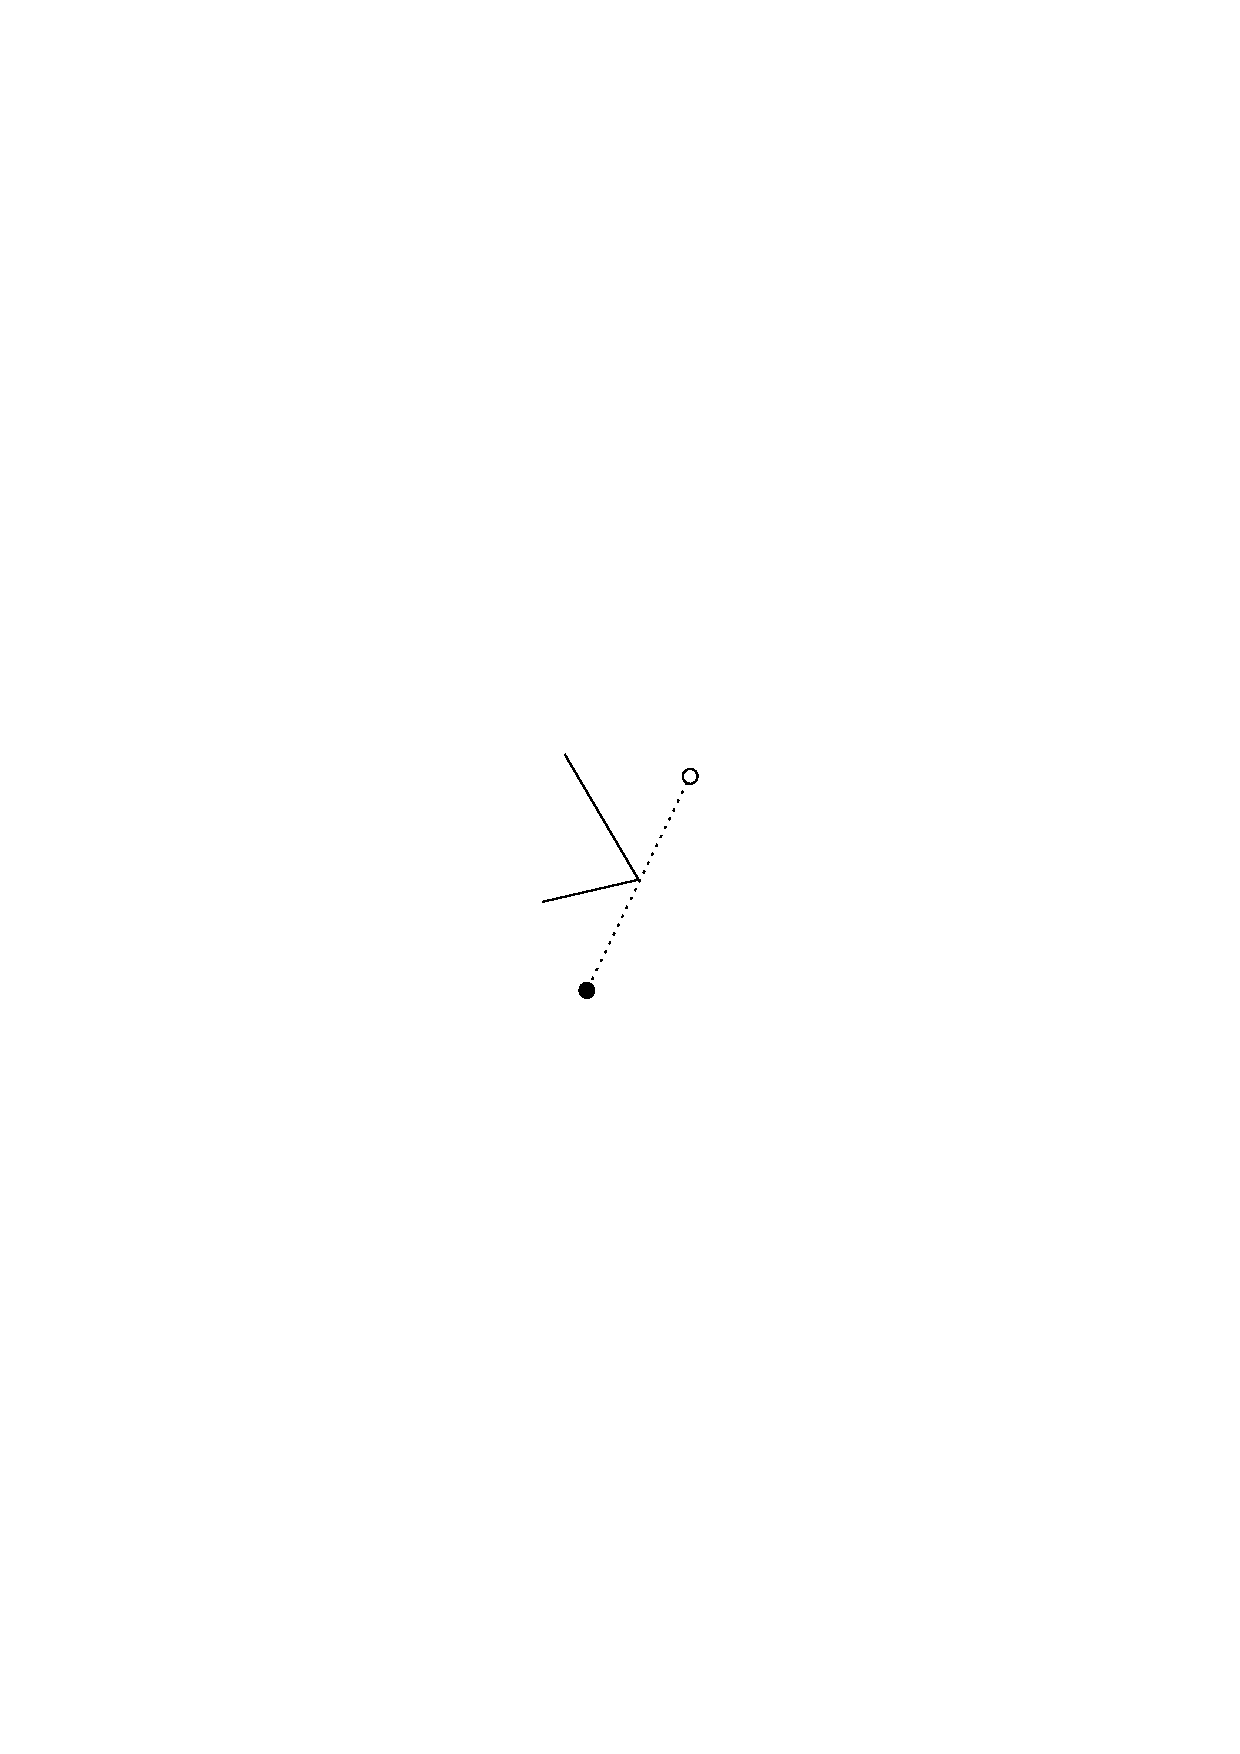
\includegraphics{\ext/spec_los}
    \caption{Special case:  the segment goes exactly through a vertex of the edge}
    \label{fig:spec_los}
  \end{figure}
\end{enumerate}

In the first case, the edge is completely ignored. In the second case,
the intersection of the segment does not count and testing will be
continued.

The results of the test depend heavily on the topological connectivity
of edges (cf.  fig.~\ref{fig:difflos}).

\begin{figure}[htbp]
  \centering
  \includegraphics{\ext/difflos}
  \caption{Different results of line-of-sight test}
  \label{fig:difflos}
\end{figure}

Here at the left subfigure (boundaries are slightly shifted for better
overview) both points are connected, whereas in the right subfigure,
the points are disconnected by both line segments.

The \lost{} does not work for more complicated cases, for instance in
case of spiral boundaries (fig.~\ref{fig:badlos}).
\begin{figure}[htbp]
  \centering
  \includegraphics{\ext/badlos}
  \caption{Line-of-sight test does not work in case of spiral edges}
  \label{fig:badlos}
\end{figure}

Here the \lost{} gives wrong results. Point 1 is actually at the same
side as the estimation point and point 2 is at another side.

Concerning the question of finding the shortest path between two
points (see section \ref{sec:Vari-calc}), we are looking for the
complete solution of this problem. For now, the \lost{} should
sufficiently work in most of the usual cases.

For \pipt{} of points we have used the InPoly routine,
which is a part of the code in  \cite{rourke:compgeom}.

\begin{quote}
  InPoly test is written by Joseph O'Rourke, contributions by Min Xu,
  June 1997.
\end{quote}

For a given point it can define, if the point
\begin{itemize}
\item lies strictly inside or outside of a polygon,
\item is a vertex of a polygon,
\item lies exactly at the edge between vertexes.
\end{itemize}

\section{Formats available for input}
\label{sec:Form-avail-input}

Boundaries can be read in two formats:
\begin{description}
\item[E00 format] -- this is supposed to be ASCII ARC/INFO coverage
  format. As this format is not officially documented by ESRI, no
  warranty can be given.

  First and second lines of a file are:
\begin{verbatim*}
EXP    Name_of_coverage
ARC
\end{verbatim*}
  
  Then every polyline (polygon) has the header

\begin{verbatim}
I_ok dummy_I dummy_I dummy_I dummy_I dummy_I I_np
\end{verbatim}
  
  x-y coordinates follow then, with either one coordinate (two
  numbers) or two coordinates (four numbers) per line. \texttt{I\_np}
  is a number of coordinates in that polyline. A polyline/polygon will
  be read in, if \texttt{I\_ok} $>0$.

  
\item[``plot'' format] -- only polylines/polygons data without header.
  
  For every polyline/polygon, the first line gives a number of points.
  x-y coordinates follow then, with either one coordinate (two
  numbers) or two coordinates (four numbers) in each line.

\end{description}


%For both formats, coordinates are given in free format (white-space
%separated, possibly with e or E exponent part).

Coverage format is automatically recognized by \texttt{EXP} as the
first word of a file.

\section{New keywords}
\label{sec:New-keywords}

\begin{enumerate}
\item \edges{}. To use like:
  
\begin{verbatim}
  edges: "file1","file2",...;
\end{verbatim}  
  Given boundary files will be read in and the boundaries will be used
  during neighborhood search. You can give both polylines and polygons.
  
\item \pip{}. To use like: 
  
\begin{verbatim}
  method: point-in-polygon;
\end{verbatim}  
  With given point locations (through \texttt{data} statement), gstat
  will search which polygons the points are in.  The output is a list
  of locations with a file number in the prediction column and a
  polygon number in the variance column of the output file. For points
  inside a polygon, this will be numbers counting  from 0.  Locations
  which are not inside of any polygon will have NA in both columns.
  
\end{enumerate}   


\section{Using \pipt{}}
\label{sec:Using-pipt}

To use \pipt{}, give through data statement the locations of points you
want to test for being inside of given \edges{}.

For this test, polylines do not have to be closed -- they are treated
as closed anyway. Points on the polyline or coincident with vertices
are assumed to be inside of the polygon.

A data point gets the number of the first of given polygons it is in,
or NA otherwise. You can parse the output with tools you have at the
hand (grep, awk, Perl\dots{}) and select points you are interested in.

\section{Using polylines with interpolation}
\label{sec:int-poly}


Edges are used for neighborhood selection after testing for
radius/maximum number of data points. The global selection will be
changed as well.

Suppose we have an estimation point (to get an interpolated/simulated
value at) and a data point. First, all relevant edges in the search
neighborhood are found. This works by comparing the bounding boxes of
all edges with the box region of the estimation point (fig.~\ref{fig:boxtest}).

\begin{figure}[htbp]
  \centering
  \includegraphics{\ext/boxtest}
  \caption{Test of edges' extents}
  \label{fig:boxtest}
\end{figure}

                                %If the estimation point lies directly at any closed polyline, this
                                %polyline is ignored.

Then, depending on the type of the polyline (open/closed), the \lost{}
or the \pipt{}  is performed for the estimation point and all data
points found so far.


During the testing, if the estimation point is found being on any
edge, this edge is skipped for further testing for this estimation
point for all data points. If a data point lies on any edge, this edge
will not be tested for this data point anymore.

The edges test is repeated for all edges found. A data point will be
used, if it passes the test for all edges.

As you can see, all testing is done by brute-force testing. So if you
have a lot of edges, with all of them relevant for most of the data
points, this will slow down interpolation/simulation a lot. Smarter
edges searching is for sure possible, for example, using line
quadtrees.  Better testing can probably be implemented in
connection with finding the shortest path between two points.



\section{Distance calculation with boundaries}
\label{sec:Vari-calc}

Both variogram calculation and interpolation depend on the
calculation of distance between two points. Without edges, this
distance is simply an Euclidean one. Taking edges into account, the
situation will be more difficult (fig.~\ref{fig:indirect}).

\begin{figure}[htbp]
  \centering
  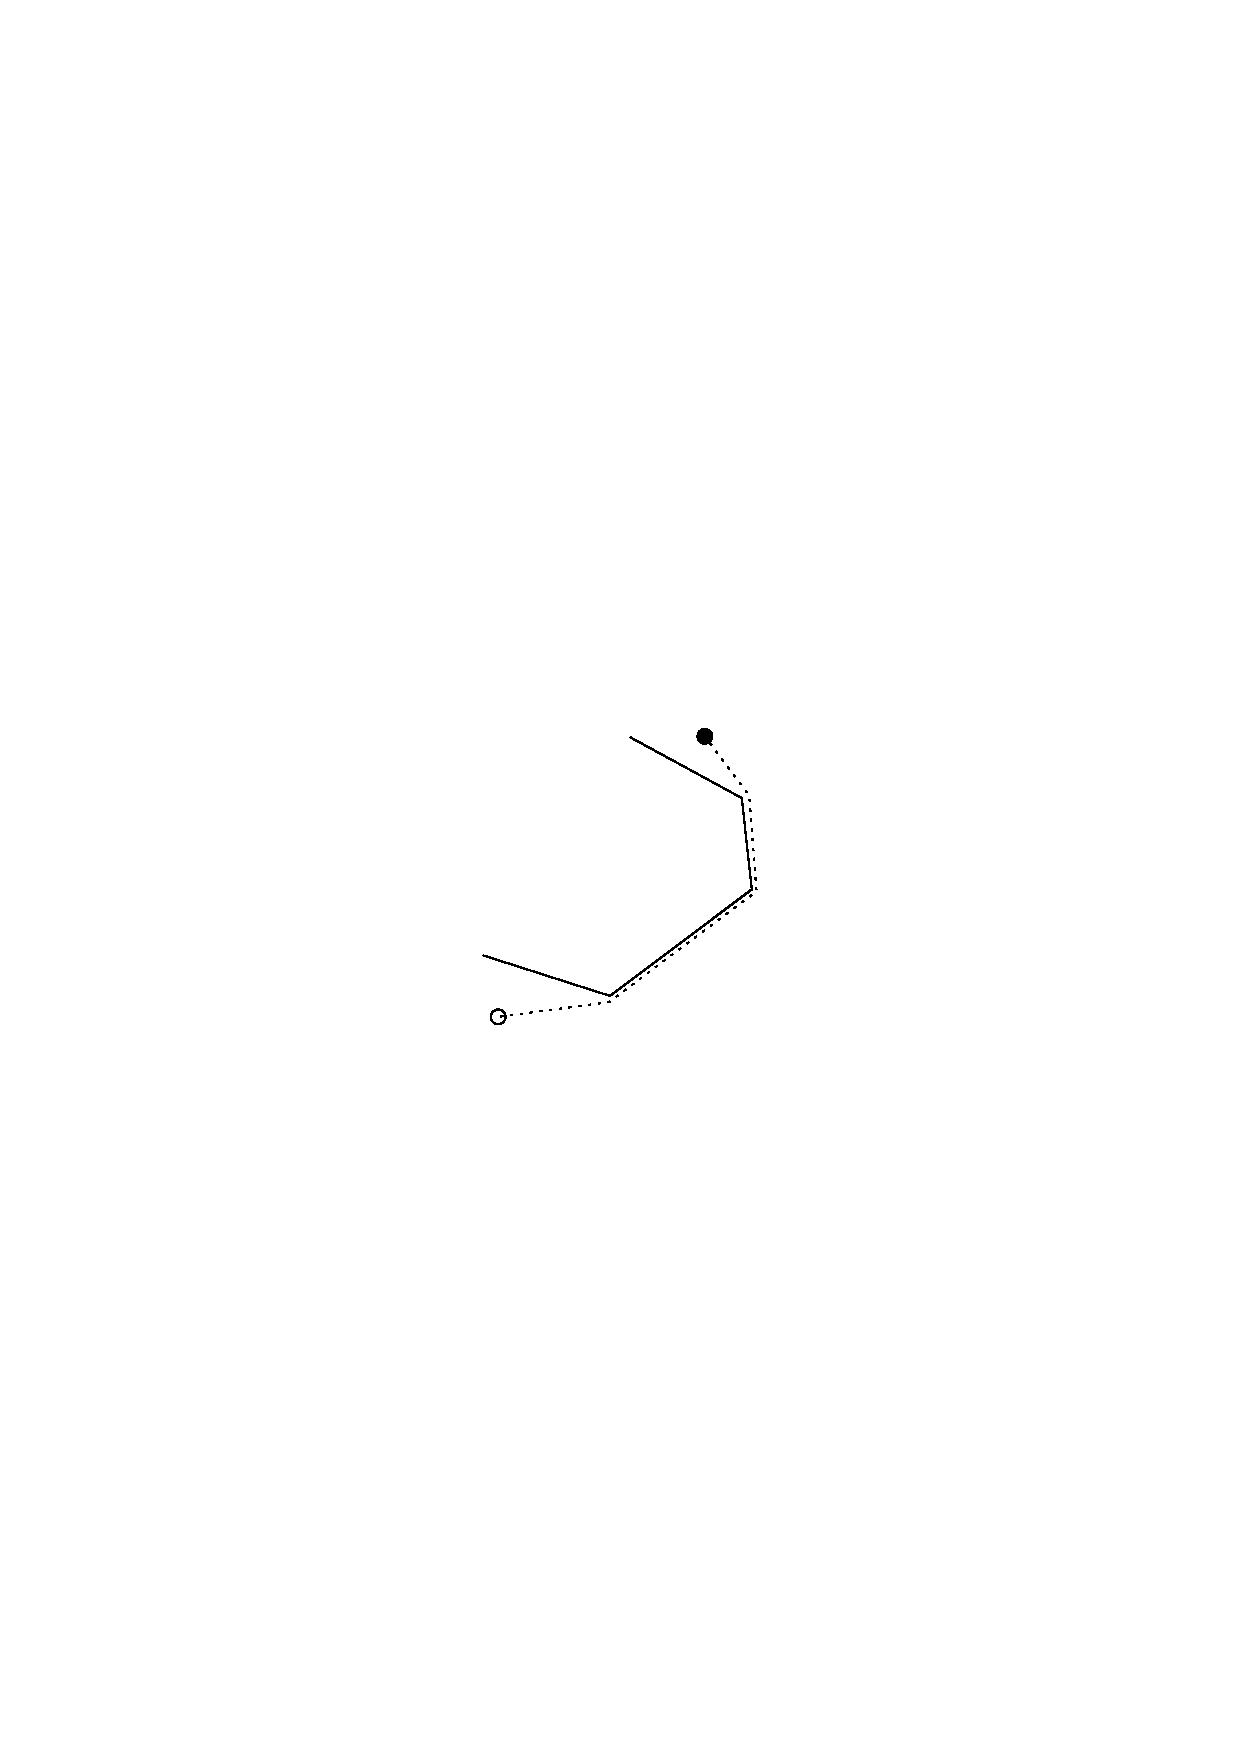
\includegraphics{\ext/dist}
  \caption{Indirect path between two points}
  \label{fig:indirect}
\end{figure}

Depending on the boundary topology, a shortest path could be not so
obvious at all.

There is a well-known solution for the problem of finding the shortest
path between points separated by some polygons (i.e. building the
connection graph and using Dijkstra's algorithm). We were not able to
find any ready solution for the case of \emph{open} polylines. So
until the solution is found, the distance between two points will be
calculated without taking boundaries into account. We suppose that the
correct solution will also eliminate the problems of the \lost.
 % by K. Malakhanov

\chapter{Trouble shooting}
\label{app:trouble}

\section{Error messages}

\subsection{From gstat}

Errors can occur in the gstat code or during the matrix operations in
the meschach matrix library. The cause of and possible solutions to the
latter are explained in the second part of this section. Following is a
list of the gstat error messages (with exit values).

\begin{codelist}
\item[\code{variable not set: ... (2)}]
the named variable should have been set in the command file.
\item[\code{variable outside valid range: ... (3)}]
the named variable is outside its valid range (e.g. negative, where it
should be positive).
\item[\code{value not allowed for: ... (4)}]
the named variable got a value that was not allowed (e.g. outside the
valid range, or in contradiction to other settings)
\item[\code{no file name set: ... (5)}]
a file name was not set where it should.
\item[\code{write failed on file `...' (6)}]
could not write the named file (e.g. no write permission, file system
full,...).
\item[\code{read failed on file `...' (7)}]
could not read the named file (e.g. file does not exist, no read
permission,...).
\item[\code{cannot read real value from `...' (8)}]
could not transform the named string into a real number.
\item[\code{cannot read integer from `...' (9)}]
could not transform the named string into an integer.
\item[\code{syntax error: ... (10)}]
a syntax error occured in the file, at the position pointed to.
\item[\code{argument option error on `...' (11)}]
the named command line argument is erroneous.
\item[\code{domain (math) error on `...' (12)}]
math domain error
\item[\code{out of dynamic memory (13)}] Memory resources exhausted.\\
Reduce problem size or increase computer resources 
(e.g. platform, memory, swap space).
\item[\code{i/o error: ... (14)}]
interactive mode cannot be combined with redirected input or output
streams.
\item[\code{no command file (15)}]
no command file was specified.
\item[\code{no user interface available (16)}]
\item[\code{error while writing to a pipe (17)}]
\item[\code{error while reading to a pipe (18)}]
\item[\code{operation not allowed in secure mode (19)}]
\item[\code{error in meschach matrix libary (20)}] followed by further
notification on what happened and hints on how this can be resolved
\item[\code{general error: ... (-1)}] and the next,
\item[\code{NULL argument in function `...' (1)}] should not occur,
please report this type of error the author (use command line option -d2).
\end{codelist}

\noindent
Other possible errors are:
\begin{codelist}
\item[\code{error during variogram fit (no exit from user interface)}]
If you specify for instance a variogram model:

\code{variogram(a): 1sph(2) + 1sph(2);}

then the two models are linearly dependent---fitting their sill will
lead to a singularity. Also, if, at a nonlinear fit, the range of a
model tends to infinity, the true model may have to be a linear model
(having one parameter), but two parameters are being fit for it---they
will then be linearly dependent and lead to a singularity during fit.
Solution: simplify the variogram model.

\end{codelist}

\subsection{From meschach}

The two most frequently encountered errors from the meschach
matrix library are:

\code{Matrix not positive definite ...} 

\noindent
or

\code{Singular matrix in function ...}

\noindent
Apart from out-of-memory errors (see above) the meschach library
terminates program execution when it encounters a matrix singularity.

These two error messages may occur:
\begin{itemize}
\item during simulation, when an
observation falls {\em almost} exactly at a simulation location.
Solution: increase the value of \iskey{zero}
\item when two observations occur at identical location occur and 
{\tt noaverage} or \iskey{average}{\tt =0} was defined in 
a {\tt \iskey{data}} definition.
Solution: remove the {\tt noaverage}, or add \iskey{average}=1
\item when a Gaussian variogram is used without a nugget effect.
Solution: add a nugget effect. 
\item when universal kriging is used (\iskey{X} and/or \iskey{d} defined),
and at some stage, usually in a local neighbourhood, one of the covariates
(\iskey{X}-variables) is constant (and therefore no longer independent
from the intercept), or dependent on another \iskey{X}-variable.
Solution: increase the neighbourhood size and make sure that
\iskey{X}-variables are {\em never} dependent.
\end{itemize}

\section{Strange results}
\label{app:strange}

\subsection*{Very strange values}
When two (or more) of the observations are at very close distant but not
at the same location, the kriging system may become {\em ill conditioned}
(i.e. unstable). Ill conditioned kriging systems may lead to exceptional
answers (unrealistically high or low values) or to error messages. The
solution to this is to replace the close observations with one new
observation (e.g. their average) or to relocate them on the same location
(so that gstat will, by default, replace them by their average).

Checking the kriging matrices for their condition number can be done
by setting \isXkey{cn\_max}{cnXmax} to an appropriate value. If the
estimated condition number of a matrix exceeds this value, a warning
message is printed and a missing value is generated.

\subsection*{Negative cokriging prediction variances}
If arbitrary coregionalizations are defined (and the command {\tt
set \iskey{nocheck}=1;} is set to allow this), than you will probably
have encountered the warning:

\code{Warning: No Intrinsic Correlation or Linear Model of\\
Coregionalization}

\noindent
or

\code{Warning: Cauchy-Schwartz violation: ...}

\noindent
After the first warning, positive definiteness of the cokriging system
cannot be guaranteed anymore and thus cokriging variances may become
anything---positive or negative, even if the variograms pass the
Cauchy-Schwartz check.


\subsection*{Unrecognised IC or LMC}

IC (intrinsic correlation) or LMC (linear model of coregionalization)
\cite{journel78,goovaerts97} are two models for a set of variograms and
cross variograms that guarantee non-negative prediction variance. Gstat
only recognises them when the order in which basic variogram models
appear in the variogram definition are identical. E.g.,

\noindent
\begin{verbatim}
variogram(a):   1   nug() + 1   sph(2);
variogram(b):   2   nug() + 1   sph(2);
variogram(a,b): 0.5 nug() + 0.8 sph(2);
\end{verbatim}

\noindent
will be recognised as LMC, but
 
\noindent
\begin{verbatim}
variogram(a):   1   nug() + 1  sph(2);
variogram(b):   1   sph(2)+ 2  nug(); # <- changed order
variogram(a,b): 0.5 nug() + 0.8sph(2);
\end{verbatim}

\noindent
will not be recognised by gstat as LMC, although it is one. Both
definitions will produce identical output.

\subsection*{Simulation speed}
Simulation may be slow. Speeding up simulations can be done by (1) a
faster machine, or (2) tuning (reduce) the neighbourhood size, especially
the radius, or (3) choosing another simulation program, or (4) modifying
the source (let me know!).

\section{The value of zero}

At several places in gstat, a result of a calculation that is very close
to zero should be treated as zero. Therefor, the value of \iskey{zero}
is set to a small positive value, and a quantity $a$ is treated as zero
when $|a| < \epsilon$, with $\epsilon$ the value of \iskey{zero}. This
applies to the following cases:
\begin{enumerate}
\item when \iskey{average} is set, data points are averaged when their
separation distance is smaller than $\epsilon$
\item when, in sequential simulation, the absolute value of the kriging
variance is smaller than $\epsilon$, it is treated as zero and ignored
for simulation (i.e., the kriging prediction is returned as the simulated
value).
\item for the calculation of difference between two maps, (-e mapdiff)
cell values are said to be different if they differ more than $\epsilon$.
\item for the calculation of point-block or block-block (generalized)
covariances, a block discretization point is shifted over distance
$\epsilon$ when it is closer than $\epsilon$ to another (discretizing)
point.
\item for the filling of the point-point (generalized) covariance
matrix during REML fitting of covariance models, an off-diagonal
point-point distances in $x$, $y$ and $z$ direction will be set to ${\rm
SIGN}(a)\epsilon$ when the separation distance between point pairs is
smaller then $\epsilon$.
\end{enumerate}

\section{Debug information}
\label{app:debug}

Although the gstat error messages are intended to clarify what went
wrong, sometimes more information is needed to solve the problem. Extra
information on various subjects can be printed during program execution,
by setting the debug level to a specific value, e.g. to 9 by the command

{\tt set debug = 9; }

\noindent
or by setting the equivalent command line option {\tt -d 9} (section
\ref{sec:clo}). All debug information (``help information'') is written
to the screen (stdout) but can be redirected to a log file by the command

{\tt set logfile = 'gstat.log'; }

\noindent
or by the command line option {\tt -l gstat.log}. Allowed values for
the debug level, and their effect are listed in table \ref{tab:debug}.

\begin{table}[ht]
\begin{tabular}{|r|p{12cm}|} \hline
{\tt debug} & {\em output} \\ \hline
{\tt 0} & suppres any output except warning and error messages \\
{\tt 1} & normal output (default): short data report, program
action and mode, program progress in \%, total execution time \\
{\tt 2} & print the value of all global variables, all files
read and written, and include source file name and line number
in error messages \\
{\tt 4} & print OLS and WLS fit diagnostics \\
{\tt 8} & print all data after reading them \\
{\tt 16} & print the neighbourhood selection for each prediction
location  \\
{\tt 32} & print (generalised) covariance matrices, design
matrices, solutions, kriging weights, etc. \\
{\tt 64} & print variogram fit diagnostics (number of iterations 
and variogram model in each iteration step) and order relation
violations (indicator kriging values before and after order relation
correction) \\
{\tt 128} & print warning on forced neighbourhoods (see \iskey{force}%
, section \ref{sec:set}) \\
{\tt 256} & print, instead of program progress in \%, for gridded
prediction or simulation the current row and column number, or else the
current record number \\
{\tt 512} & print block (or area) discretization data for each
prediction location \\ \hline
\end{tabular}
\label{tab:debug}
\caption{values for debug and their output}
\end{table} 

To combine options, their values are summed. For instance, setting the
debug level to 3 invokes both levels 1 and 2; setting it to 1023 would
invoke them all. (Note that in certain circumstances, the log file size
can become huge.)

\subsection*{Plotting kriging weights}
% kriging.weights @SubIndex { weights, plotting }
% plotting.kriging @Index { plotting kriging weights }

When gstat is used for kriging prediction and the plot file name is
defined, with for instance the command:

{\tt set plotfile='plot.gp';}

\noindent
then kriging weights are printed to the plot file is such a way that
they can, for each prediction location, be plotted with gnuplot, using

{\tt gnuplot plot.gp }

The variable \iskey{plotweights} can be set to express kriging weights
using different symbol sizes, its value expresses the range of sizes.

The steps of saving plot commands to file and starting gnuplot may be 
combined on operating systems that support pipes, using:

{\tt set plotfile='| gnuplot';}

assuming that the gnuplot executable is in the current search path.

\chapter{Grid map and data formats}
\label{app:formats}

\section{PCRaster maps}
Input
\htmladdnormallink{PCRaster}{http://pcraster.geog.uu.nl/} maps
should be readable as REAL4 maps. This implies that any value scale,
and all cell representations except REAL8, are allowed as input maps.
Output maps are written as REAL4 scalar maps, except for maps resulting
from indicator simulation (UINT1 scalar maps). Old PCRaster (version 1)
maps are supported when gstat is compiled with \verb|CSF_V1| defined,
and linked to the version 1 csf library. (Support for version 1 may not
be maintained in the future.)

\section{Idrisi data and maps}

\htmladdnormallink{Idrisi}{http://www.clarklabs.org/} file names should be
given without extensions: gstat assumes the extensions (.dvc, .vec, .doc,
.img) to be file-type specific. For instance, when a mask is defined as

\code{mask: 'maskmap';}

\noindent
then gstat assumes the files \code{maskmap.doc} and \code{maskmap.img} to
be present and in the correct idrisi format.

Data can be read from idrisi point files (extensions \code{.dvc} and
\code{.vec}). In the \code{.dvc} file, the field \code{id type} should
be \code{real}, \code{file type} should be \code{ascii} and \code{object
type} should be \code{point}.

Data or grid maps can be read from idrisi image files (extensions
\code{.doc} and \code{.img}). In the \code{.doc} file, the field
\code{data type} should be \code{real}, \code{byte} or \code{integer},
the field \code{file type} should be \code{ascii} or \code{binary};
the fields \code{colums}, \code{rows}, \code{min X}, \code{max Y} and
\code{resolution} should all be set (\code{resolution} must be holding
the cell size).

\section{ArcInfo/Arcview grid maps}
\subsection{asciigrid}

\htmladdnormallink{ArcInfo}{http://www.esri.com/} (or ArcView)
Asciigrid maps are single ascii files, starting with a number
of header lines, followed by the grid cell values (row-wise, from
left-to-right). The header lines ave a field name and a value. Field
names are pretty much self-explanatory, they are:
\code{ncols},
\code{nrows},
\code{cellsize},
\code{xllcenter} or \code{xllcorner},
\code{yllcenter} or \code{yllcorner}, and (optional)
\code{nodata\_value}.

\subsection{floatgrid}
A floatgrid map \code{maskmap} consist of two files: one ascii file with
the name \code{maskmap.hdr} that contains the grid map topology (as the
asciigrid header), and a binary file named either \code{maskmap.flt}
or \code{maskmap}, containing the cell values. Specify only the file name
without the \code{.hdr} or \code{.flt} extension in gstat commands. Field
names in the header file are:
\code{ncols},
\code{nrows},
\code{cellsize},
\code{xllcenter} or \code{xllcorner},
\code{yllcenter} or \code{yllcorner},
\code{byteorder},
and (optional) \code{nodata\_value}.
The field \code{byteorder} should have value \code{lsbfirst} for byte
order of little endian processors (least significant byte first, like
INTEL), or else \code{msbfirst} (HP-PA and the like). 

From version 2.1 on, gstat adds by default the \code{.flt} extension to
the binary grids file name to facilitate importing in ArcView (with 3D
or spatial analyst).

\section{ER-Mapper maps}

\htmladdnormallink{ER-Mapper}{http://www.ermapper.com/}
support was contributed by \htmladdnormallink{Steve
Joyce}{mailto:steve.joyce@resgeom.slu.se}, who wrote the following about
it on Fri, 2 Jan 1998:

ER-Mapper provides a c-function library for programmers to read and
write datafiles in a standard way. Maybe you remember my first version
used this library, but linking gstat together with ER-Mapper.lib was
just an enormous pain in the ass. It turns out, ER-Mapper raster files
are fairly straightforward anyway, with a separate ASCII header and
binary data file. So the current version reads and writes the ER-Mapper
files directly without using ermapper.lib. This may cause it to fail
for future versions of ER-Mapper, but I can live with that.

ER-Mapper raster files can be multi-channel--I check the number
of channels on input files and bail out if there is more than one.
Maybe sometime we can set up the data specification syntax to include
a channel as you talked about before.

ER-Mapper files can specify to skip a number of bytes in the binary
file--I don't take care of this, but check the file size consistencey
of the binary file.

ER-Mapper header binary files can have a different root name than the
header--I don't take care of this, and force them to be the same.

ER-Mapper data types can be signed or unsigned chars, ints (16 or 32
bits), 4-byte real or 8-byte double. I read all formats and cast into
4-byte real for sorage in the gstat gridmap. I always write 4-byte real.

Byte order can be specified in ER-Mapper raster files--I check for it
and reorder as necessary.

The ER-Mapper coordinate origin can be at an arbitrary fractional pixel
position--I correct it to be the upper left corner of the upper left
pixel in the grid.

ER-Mapper coordinates can be either Easting/Northing, Long/Lat, or
Raw(X-Y). I do a strict check for 'EN' coordinates, because they match
the definition used in gridmaps. RAW coordinates have positive 'y' going
down (same as cell coordinates) whereas EN coordinates have positive
'y' going up.

\section{GMT grid maps}

\htmladdnormallink{GMT}{http://imina.soest.hawaii.edu/gmt/} grid maps are 
basically \htmladdnormallink{netcdf}{ftp://unidata.ucar.edu/pub/netcdf/}
files. Gstat only includes GMT support when it is linked with the netcdf
library. This library is detected automatically by the configure script
(section \ref{sec:compiling}), or it is added when configure is invoked as

\code{./configure --with-netcdf}

GMT map support was contributed by \htmladdnormallink{Konstantin
Malakhanov}{mailto:kosta@iwwnt.iwwl.rwth-aachen.de} who wrote about it:

``And last but not least: I write here all limitations of using GMT 
grids with GSTAT :-

\begin{enumerate}
\item GMT grids can be centered at pixels or at nodes. GSTAT grids
are centered at pixels, so node-wise GSTAT grids will be converted
to pixel-centered. GMT grids from GSTAT are always pixel-centered.
Convertation could be made in two ways: either decrease the number
of rows and columns by one and set pixel values to mean (or median,
or what you like at most) value of 4 nodes (this changes values, but
preserves boundaries of grid) or extent grid limits to half cell size
to west/east/north/south and use nodes as centers of new pixels (this
preserves values, but slightly changes the limits of grids). I implemented
the second way, so if you have GMT node-centered grid as mask, then the
extensions of result grid from gstat will be one cell size bigger in X-
and Y-directions!

\item GMT grids can have multiplication factor and an add offset for
z-values. As GSTAT grid definition does not allow for that, GMT grid
values with factor different from 1.0 and/or value offset different from
0.0 will be accordingly transformed during the loading. (Comment: for
reasons I cannot understand GMT grids have sometimes factor 0.0 which
makes no sense. So factor==0.0 will be treated as 1.0). GSTAT grids in
GMT format always have factor== 1.0 and value offset==0.0.

\item GMT system allows for rectangular coordinate system or for
geographical projections, but there is no way to detect it from grid
itself (in GMT commands , projection is almost always supplied as one
of arguments by user). So the way GMT grids are treated is defined by
user and not stored in a grid. That means that using GSTAT for grids
which are supposed to have longitude/lattitude coordinates WILL give
results, but these results are useless as spheroid of Earth is not taken
into account and it means by no way that GSTAT can interpolate/simulate
over sphere in geographical projections (if one needs such things, take
a look at Spherekit at http://www.ncgia.ucsb.edu/pubs/spherekit). So I
didn't follow this branch further.

\item GMT grid definition has fields for names of x-,y-,z-units. These
fields are ignored at reading and will be set to " " in the result grid.

\item GMT grids can have complex z-values. This is neither checked for
nor used!''
\end{enumerate}

\section{Surfer grid maps}

Gstat now supports
\htmladdnormallink{Surfer}{http://www.goldensoftware.com/} ascii (DSAA)
grids. Missing values are stored as a value outside the data range (given
in the file header). In gstat command files, grid map names should never
have an extension (leave the {\tt .grd} out).

\ifpdf
% \phantomsection
\newpage
\pdfbookmark[0]{Bibliography}{bibliography}
\fi

\addcontentsline{toc}{chapter}{Bibliography}

\bibliography{gstat}
\bibliographystyle{plainnat}

\ifpdf
% \phantomsection
\newpage
\pdfbookmark[0]{Index}{index}
\fi

\addcontentsline{toc}{chapter}{Index}

\printindex

\end{document}
